% !TEX root = ../G-design.tex
\section{機能概要}\label{sec:overview}
\subsection{ユーザ共通機能}\label{subsec:common}
%======================================================================
本項では, ゲスト（会員でないユーザ）と会員ユーザに共通する機能について述べる.
各機能の処理の流れは, ユーザとシステムの2つのレーンに分けたアクティビティ図で示す.

%----------------------------------------------------------------------
\subsubsection{初回選択}\label{subsec:first-choice}
%----------------------------------------------------------------------
アプリ利用者は, 最初に「ゲスト利用」「ログイン」「新規会員登録」のいずれかを選択する.
ゲスト利用を選択した場合の流れを図\ref{fig:guest}に示す.
なお, ログインおよび新規会員登録については, \ref{subsec:member}で詳しく説明する.

\begin{figure}[H]
  \centering
  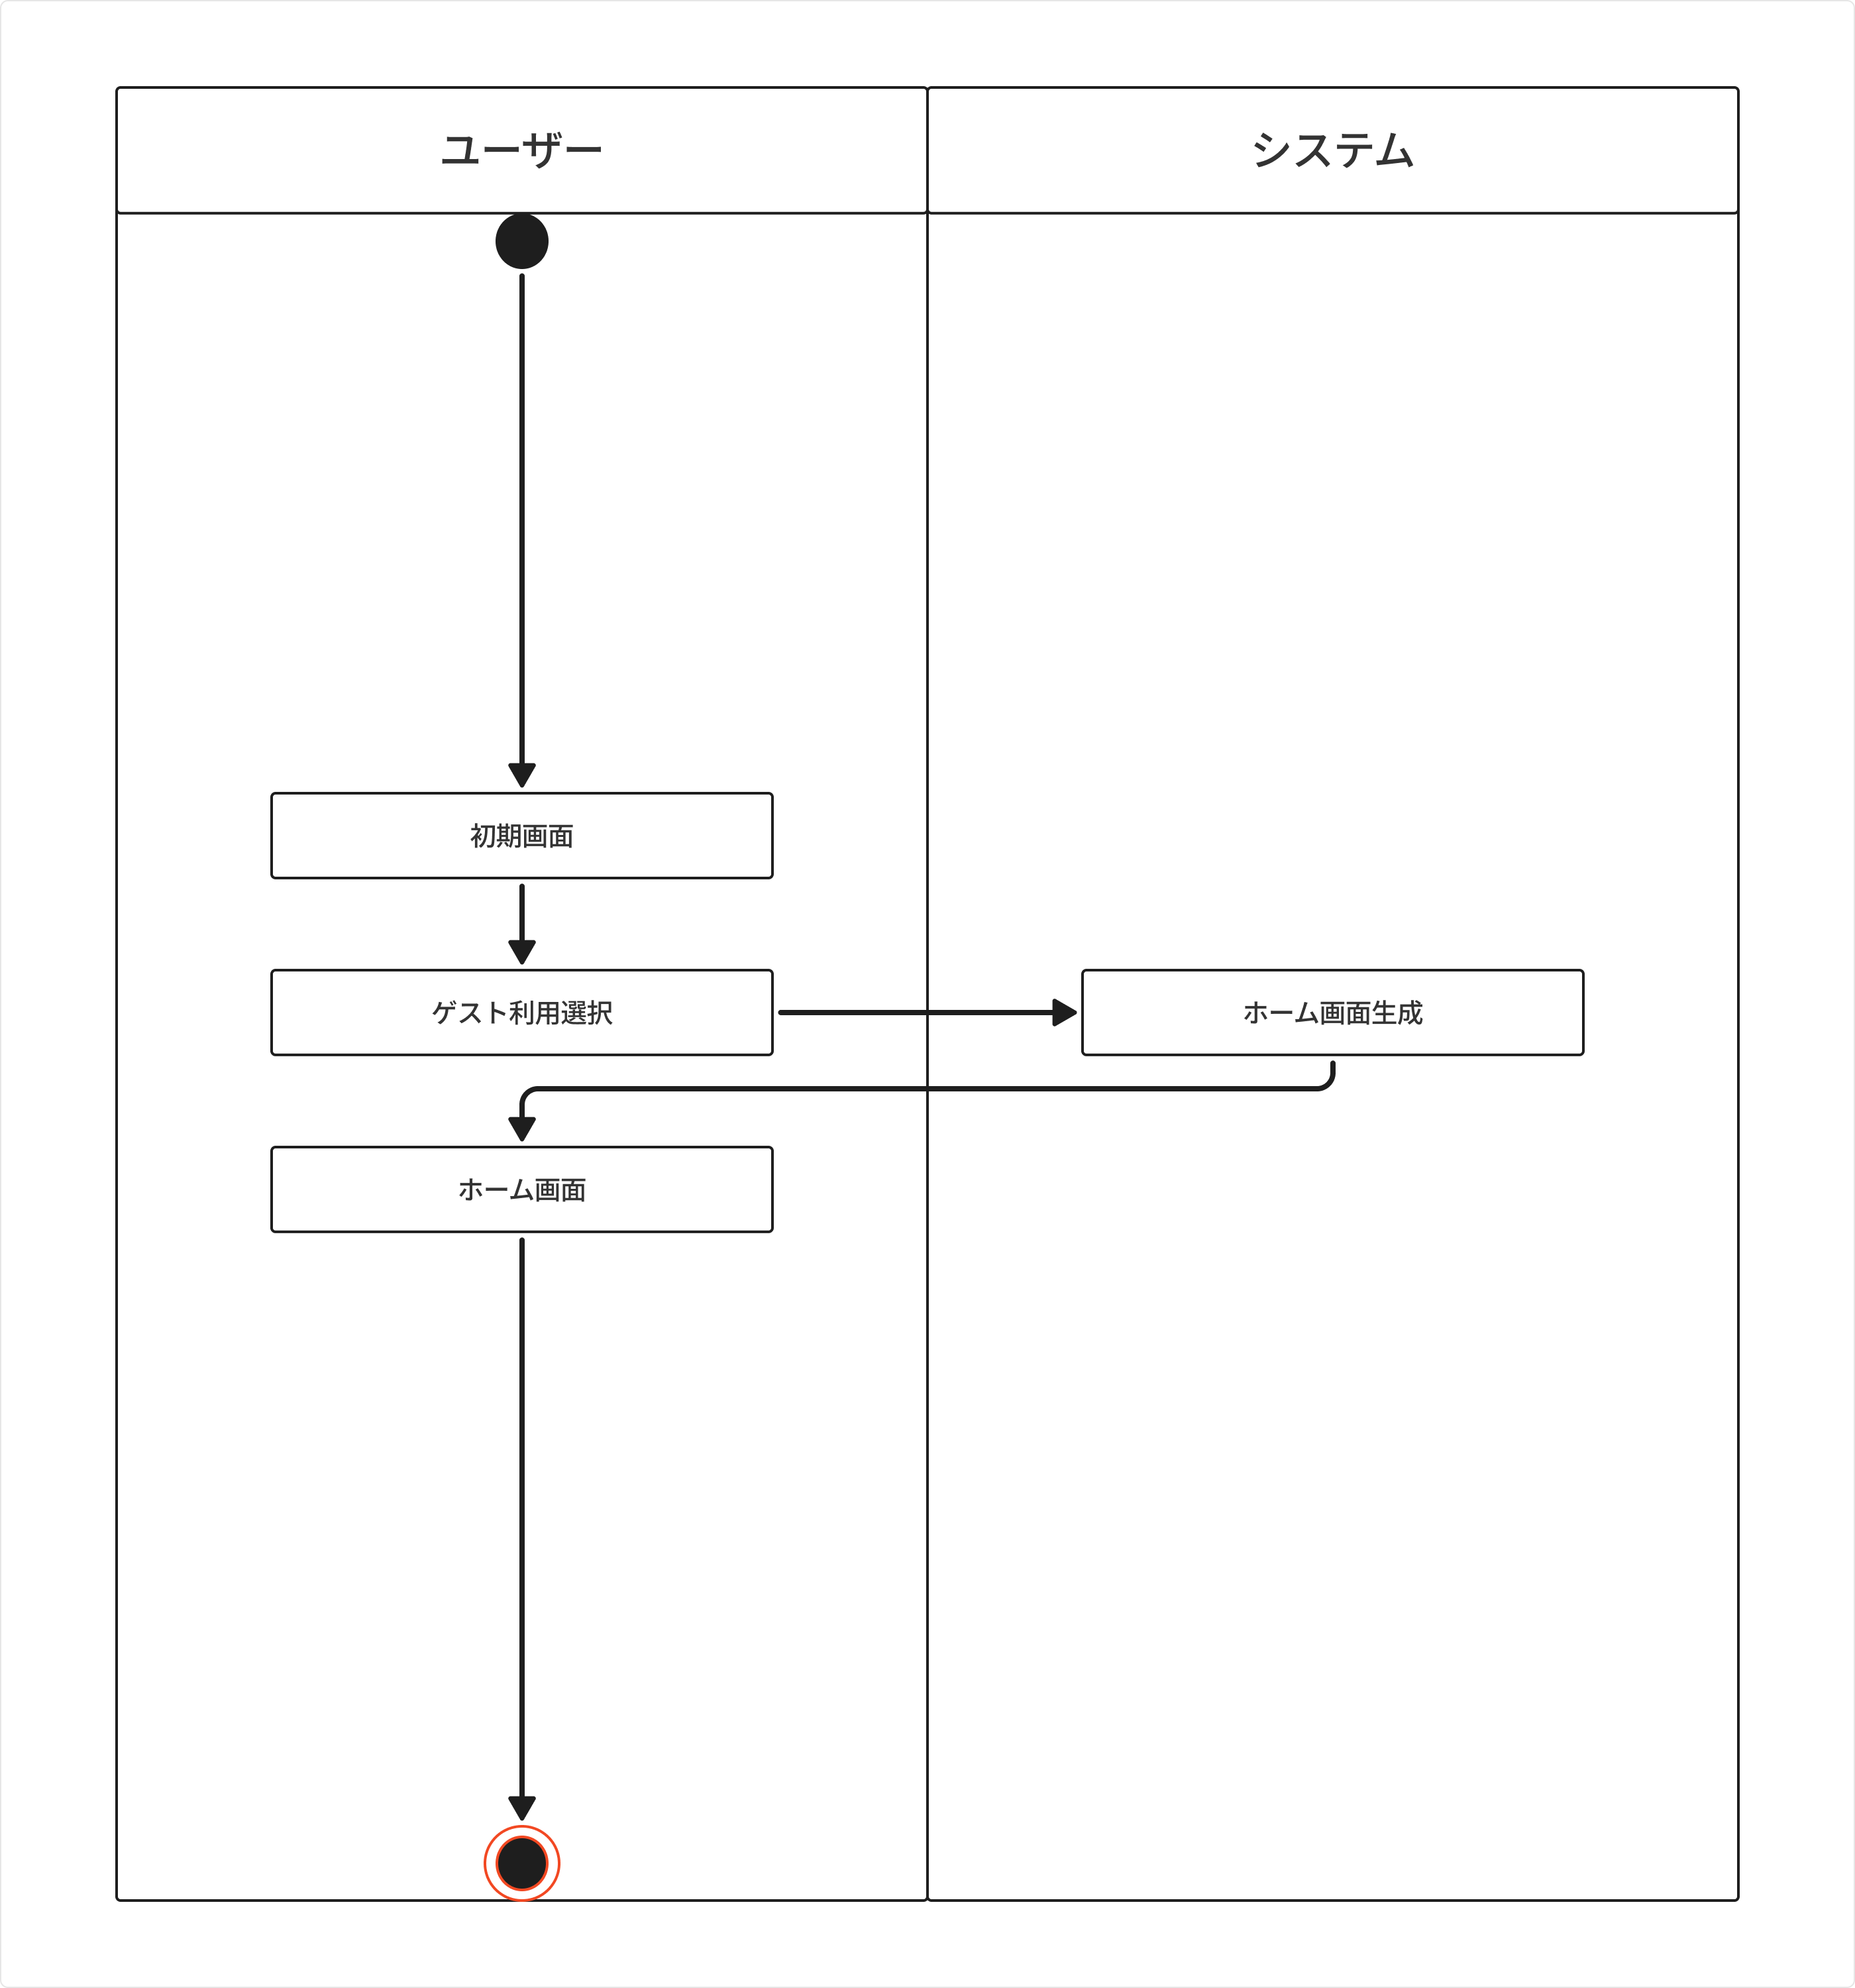
\includegraphics[width=0.6\linewidth]{chapters/images/guest.png}
  \caption{初回選択（ゲスト利用）のアクティビティ図}
  \label{fig:guest}
\end{figure}

%----------------------------------------------------------------------
\subsubsection{チュートリアル機能}\label{subsec:tutorial}
%----------------------------------------------------------------------
利用者が初めてみる画面に遷移した場合, その画面のチュートリアルが作動する.
すべてのチュートリアルにはスキップ機能を設け, スキップを選択した場合は, その画面のチュートリアルを終了したものとして扱う.
また, チュートリアルはホーム画面の「ヘルプ」から「チュートリアル」ボタンを選択することで, いつでも見返すことができる.

図\ref{fig:tutorial1}に, ホーム画面から検索を経て投稿を閲覧するまでのチュートリアルの流れを示す.

図\ref{fig:tutorial2}に, ヘルプ画面および設定画面のチュートリアルの流れを示す.

\begin{figure}[H]
  \centering
  \begin{minipage}[t]{0.48\linewidth}
    \centering
    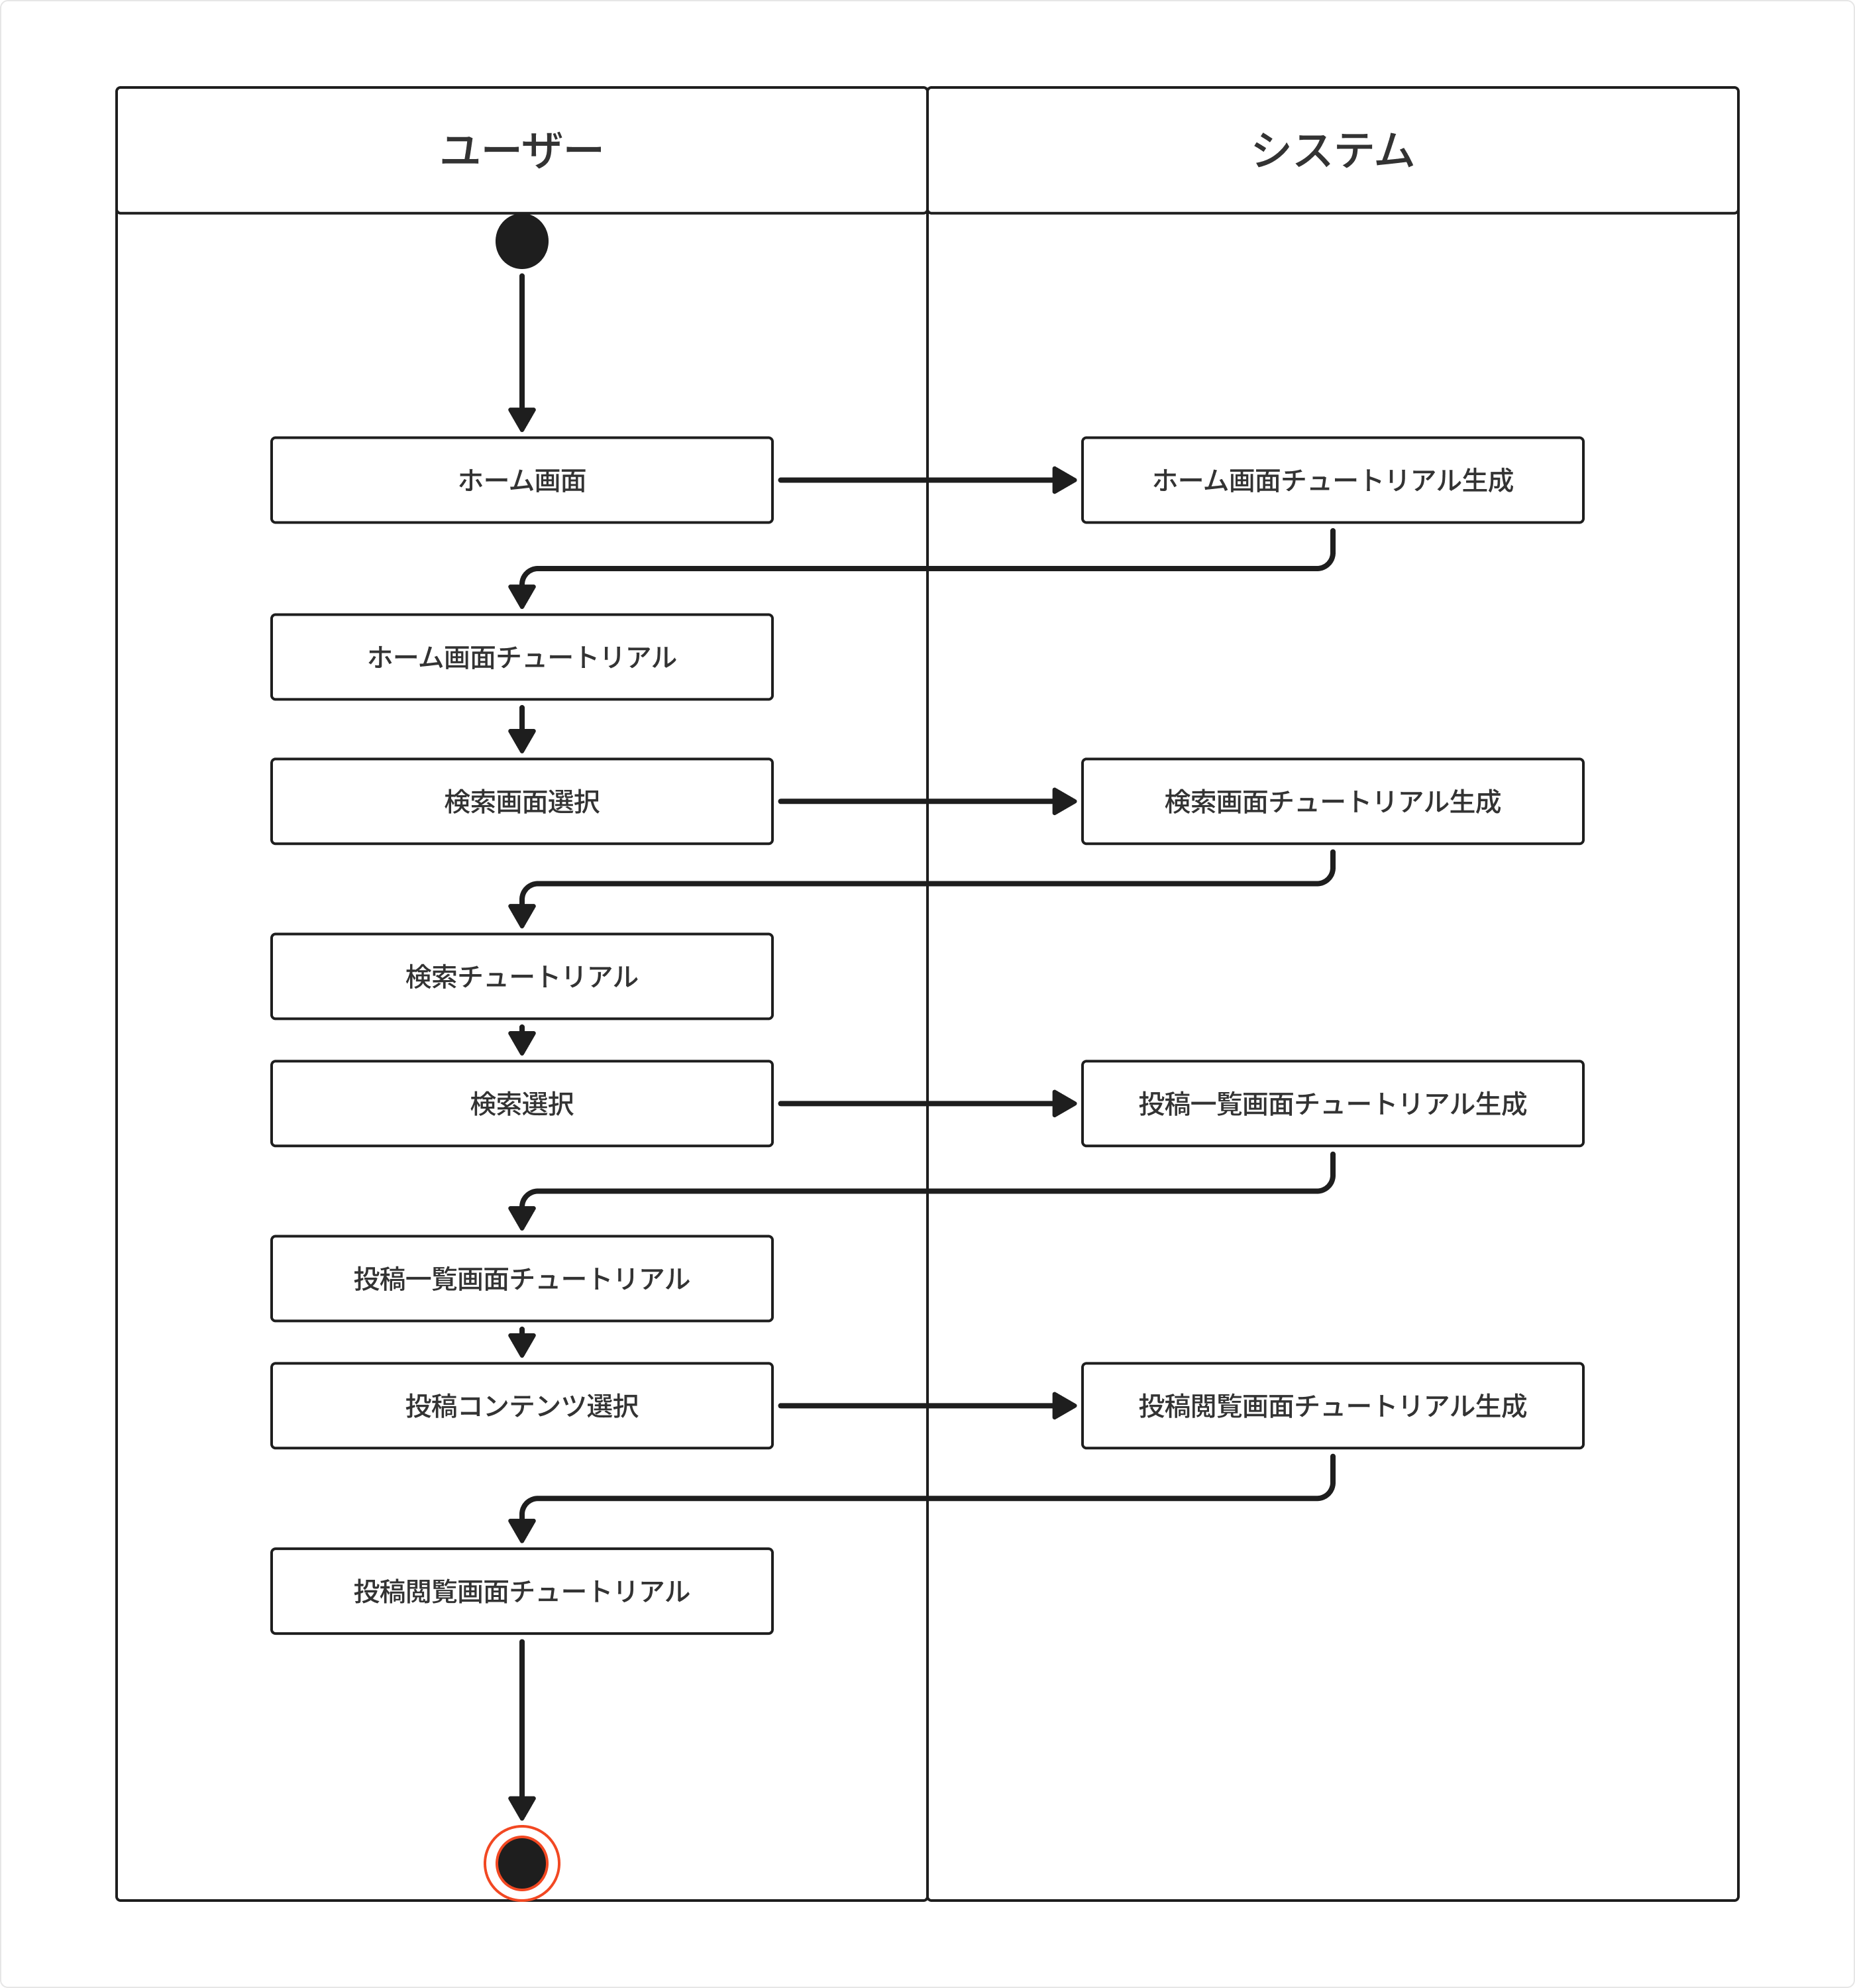
\includegraphics[width=\linewidth]{chapters/images/tutorial1.png}
    \caption{利用者チュートリアル1（ホーム・検索・投稿閲覧）}
    \label{fig:tutorial1}
  \end{minipage}
  \hfill
  \begin{minipage}[t]{0.48\linewidth}
    \centering
    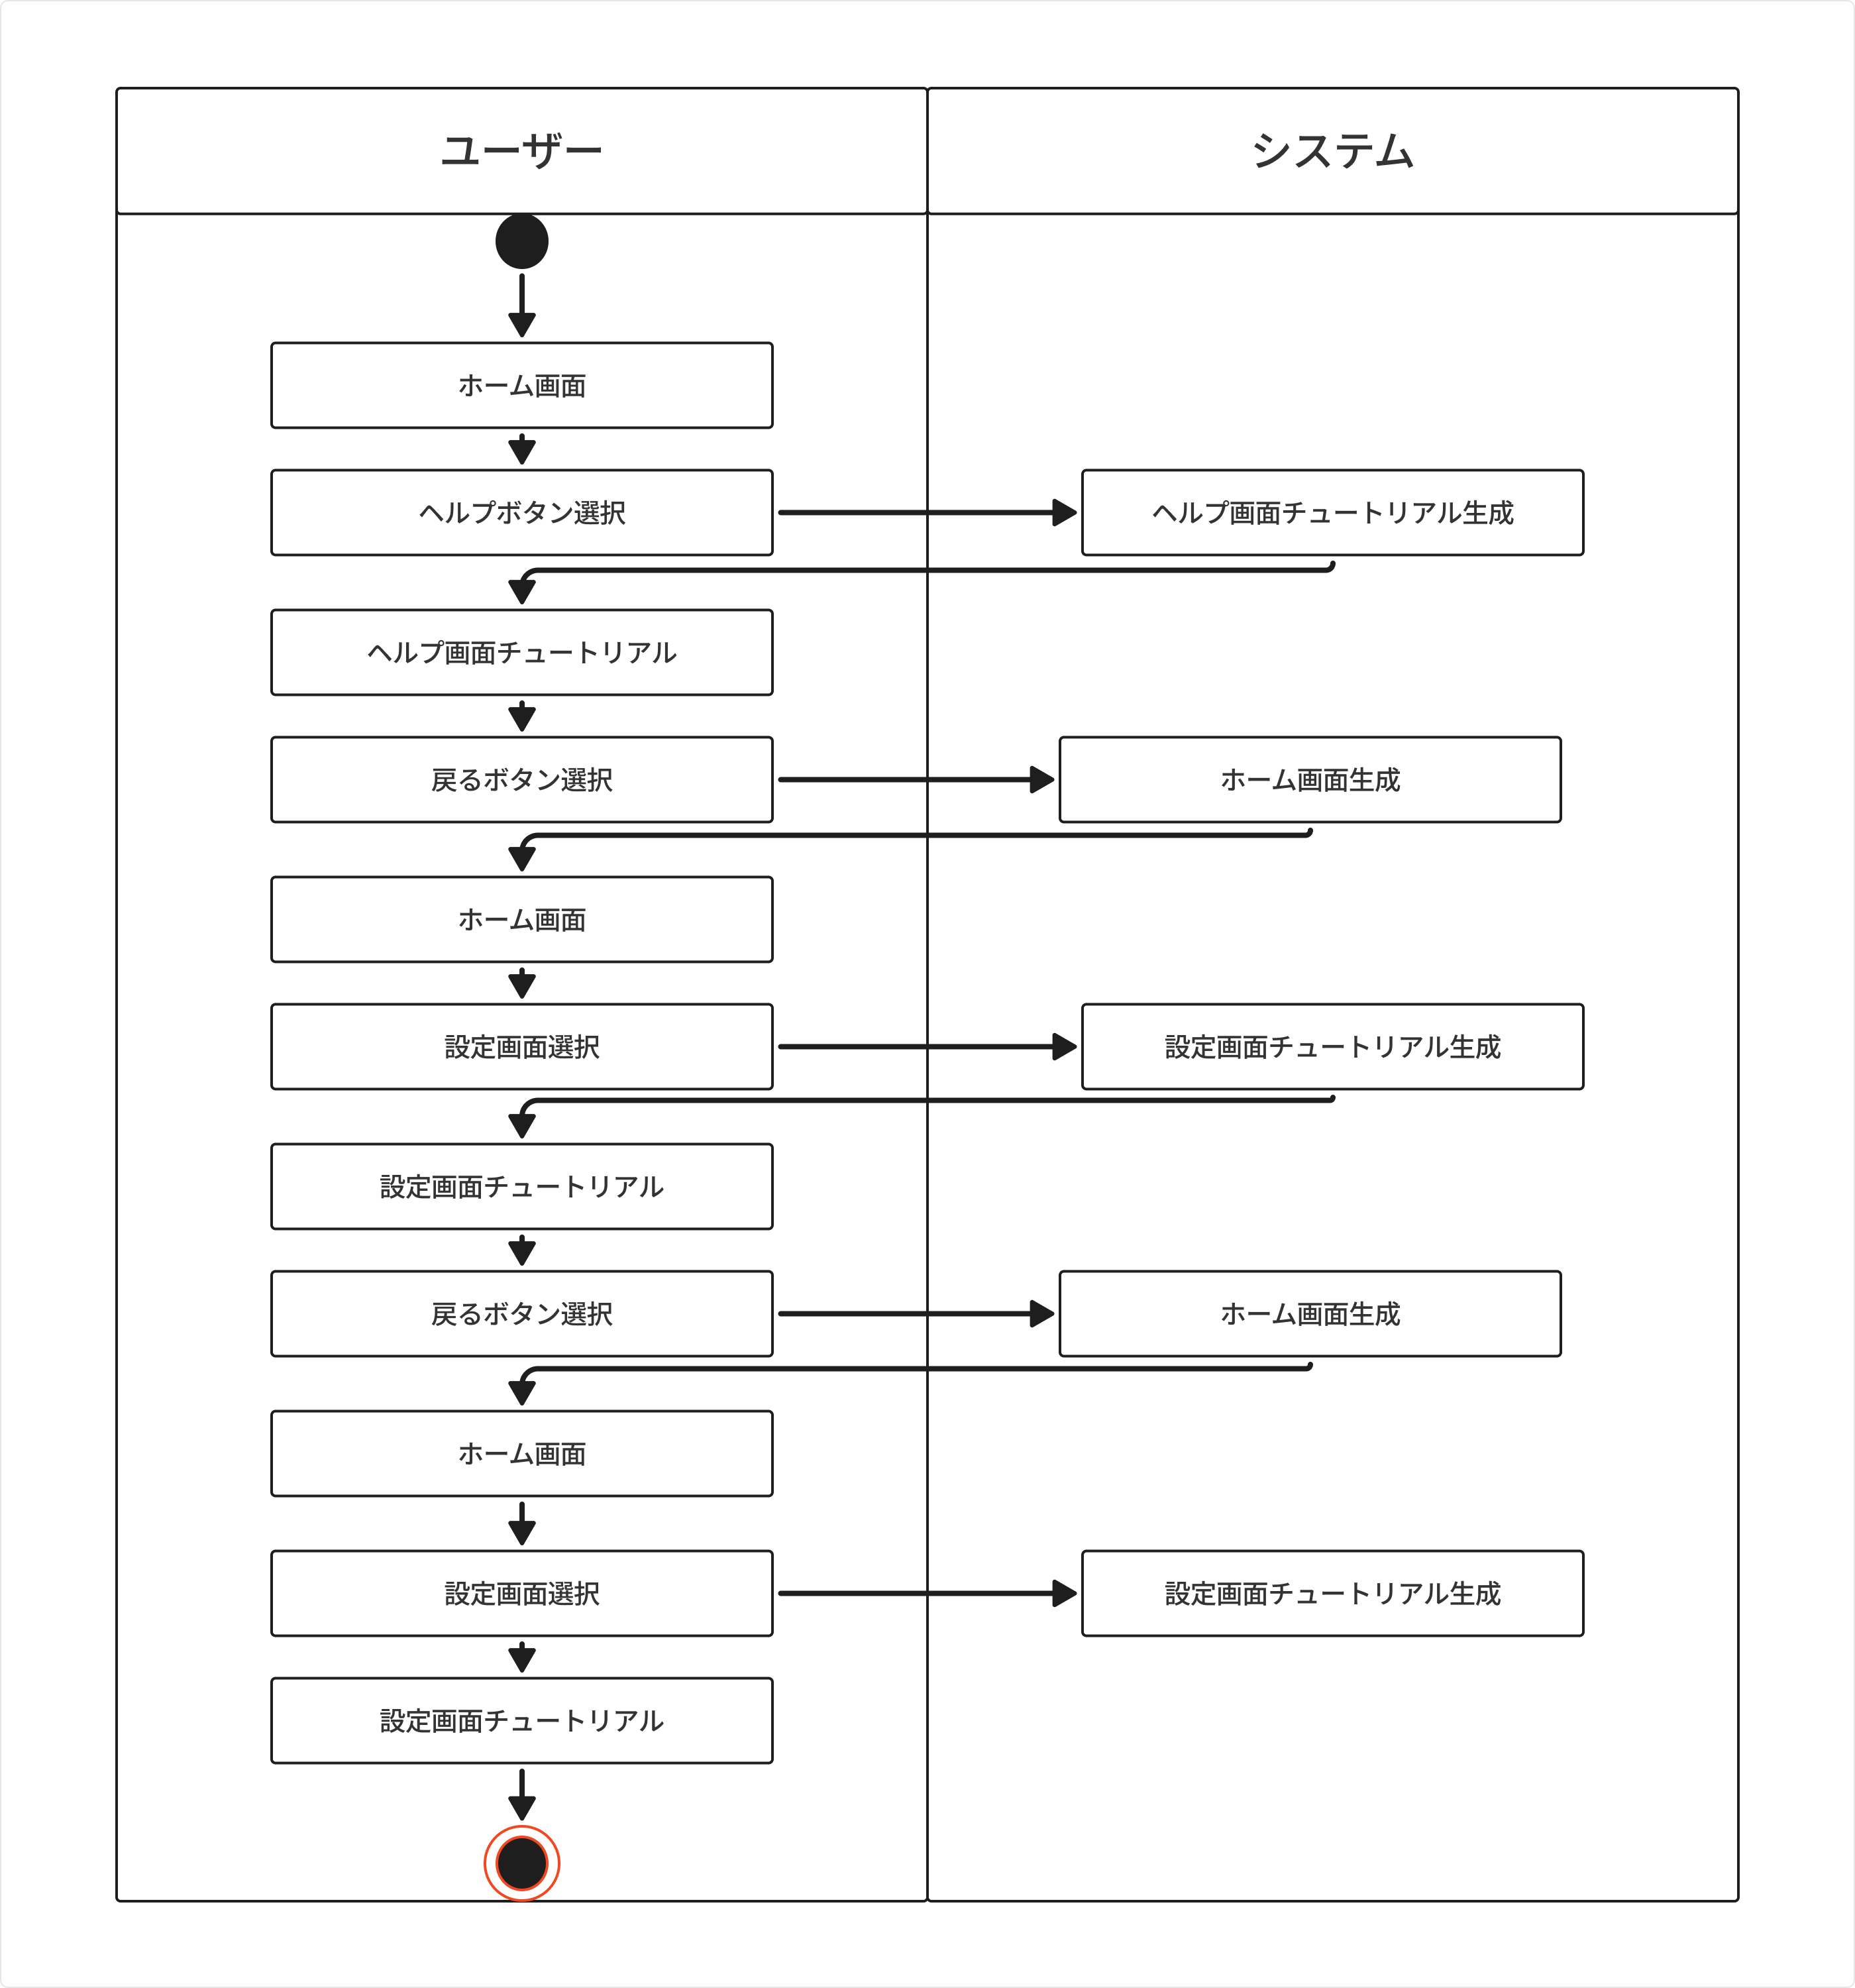
\includegraphics[width=\linewidth]{chapters/images/tutorial2.png}
    \caption{利用者チュートリアル2（ヘルプ・設定）}
    \label{fig:tutorial2}
  \end{minipage}
\end{figure}

%----------------------------------------------------------------------
\subsubsection{検索機能}\label{subsec:search}
%----------------------------------------------------------------------
投稿の検索は, 次の3通りの方法で行うことができる.
\begin{itemize}
  \item 文字または音声の入力による検索
  \item カテゴリから選ぶ検索
  \item AI検索
\end{itemize}
検索画面には, 利用者が検索したワードを集計し, 上位5件をトレンド検索ワードとして表示する.
検索結果画面には, キーワードとの関連度が高い順に投稿を一覧で表示する.
一覧を最後までスワイプすると「YouTubeで検索」が表示され, これを選択するとYouTubeで再検索できる.

\paragraph{文字/音声検索}
図\ref{fig:search-text}に文字/音声検索の流れを示す.

\paragraph{カテゴリ検索}
図\ref{fig:search-category}にカテゴリ検索の流れを示す.

\paragraph{AI検索}
図\ref{fig:search-ai}にAI検索の流れを示す.

\paragraph{再検索（YouTubeで検索）}
図\ref{fig:research}に再検索の流れを示す.

\begin{figure}[H]
  \centering
  \begin{minipage}[t]{0.35\linewidth}
    \centering
    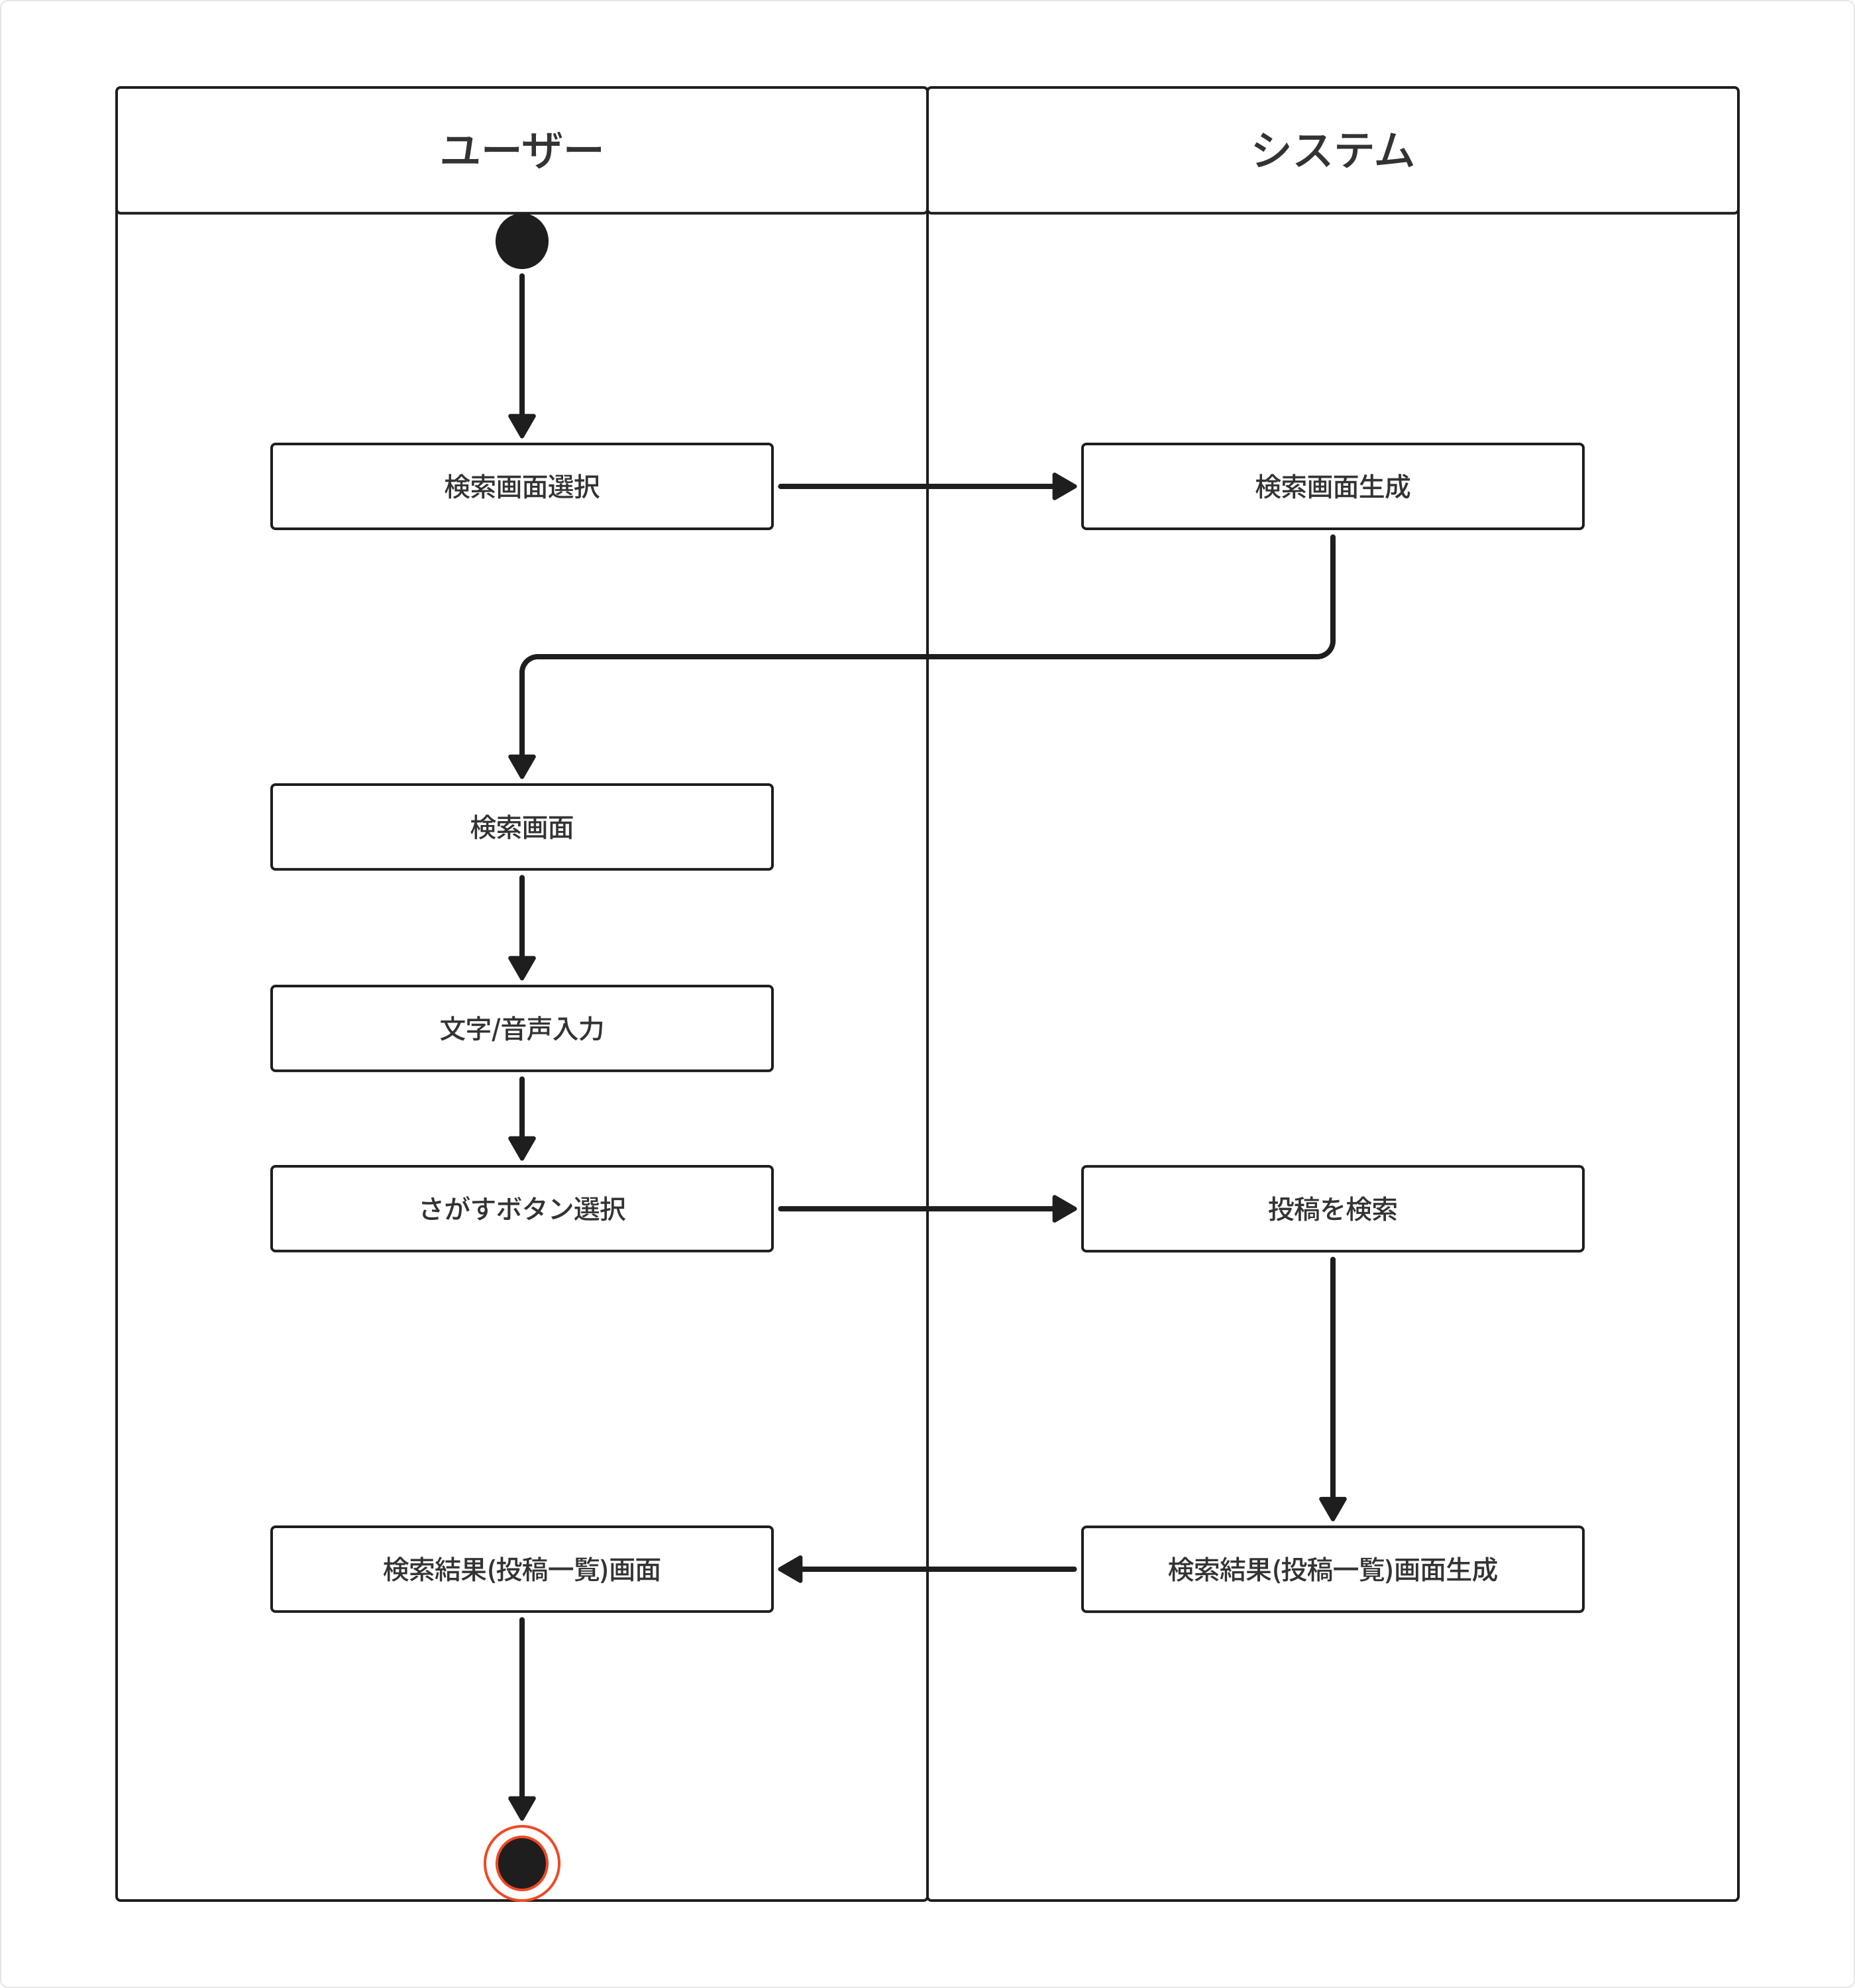
\includegraphics[width=\linewidth]{chapters/images/search_text.png}
    \caption{文字/音声検索機能のアクティビティ図}
    \label{fig:search-text}
  \end{minipage}
  \hfill
  \begin{minipage}[t]{0.35\linewidth}
    \centering
    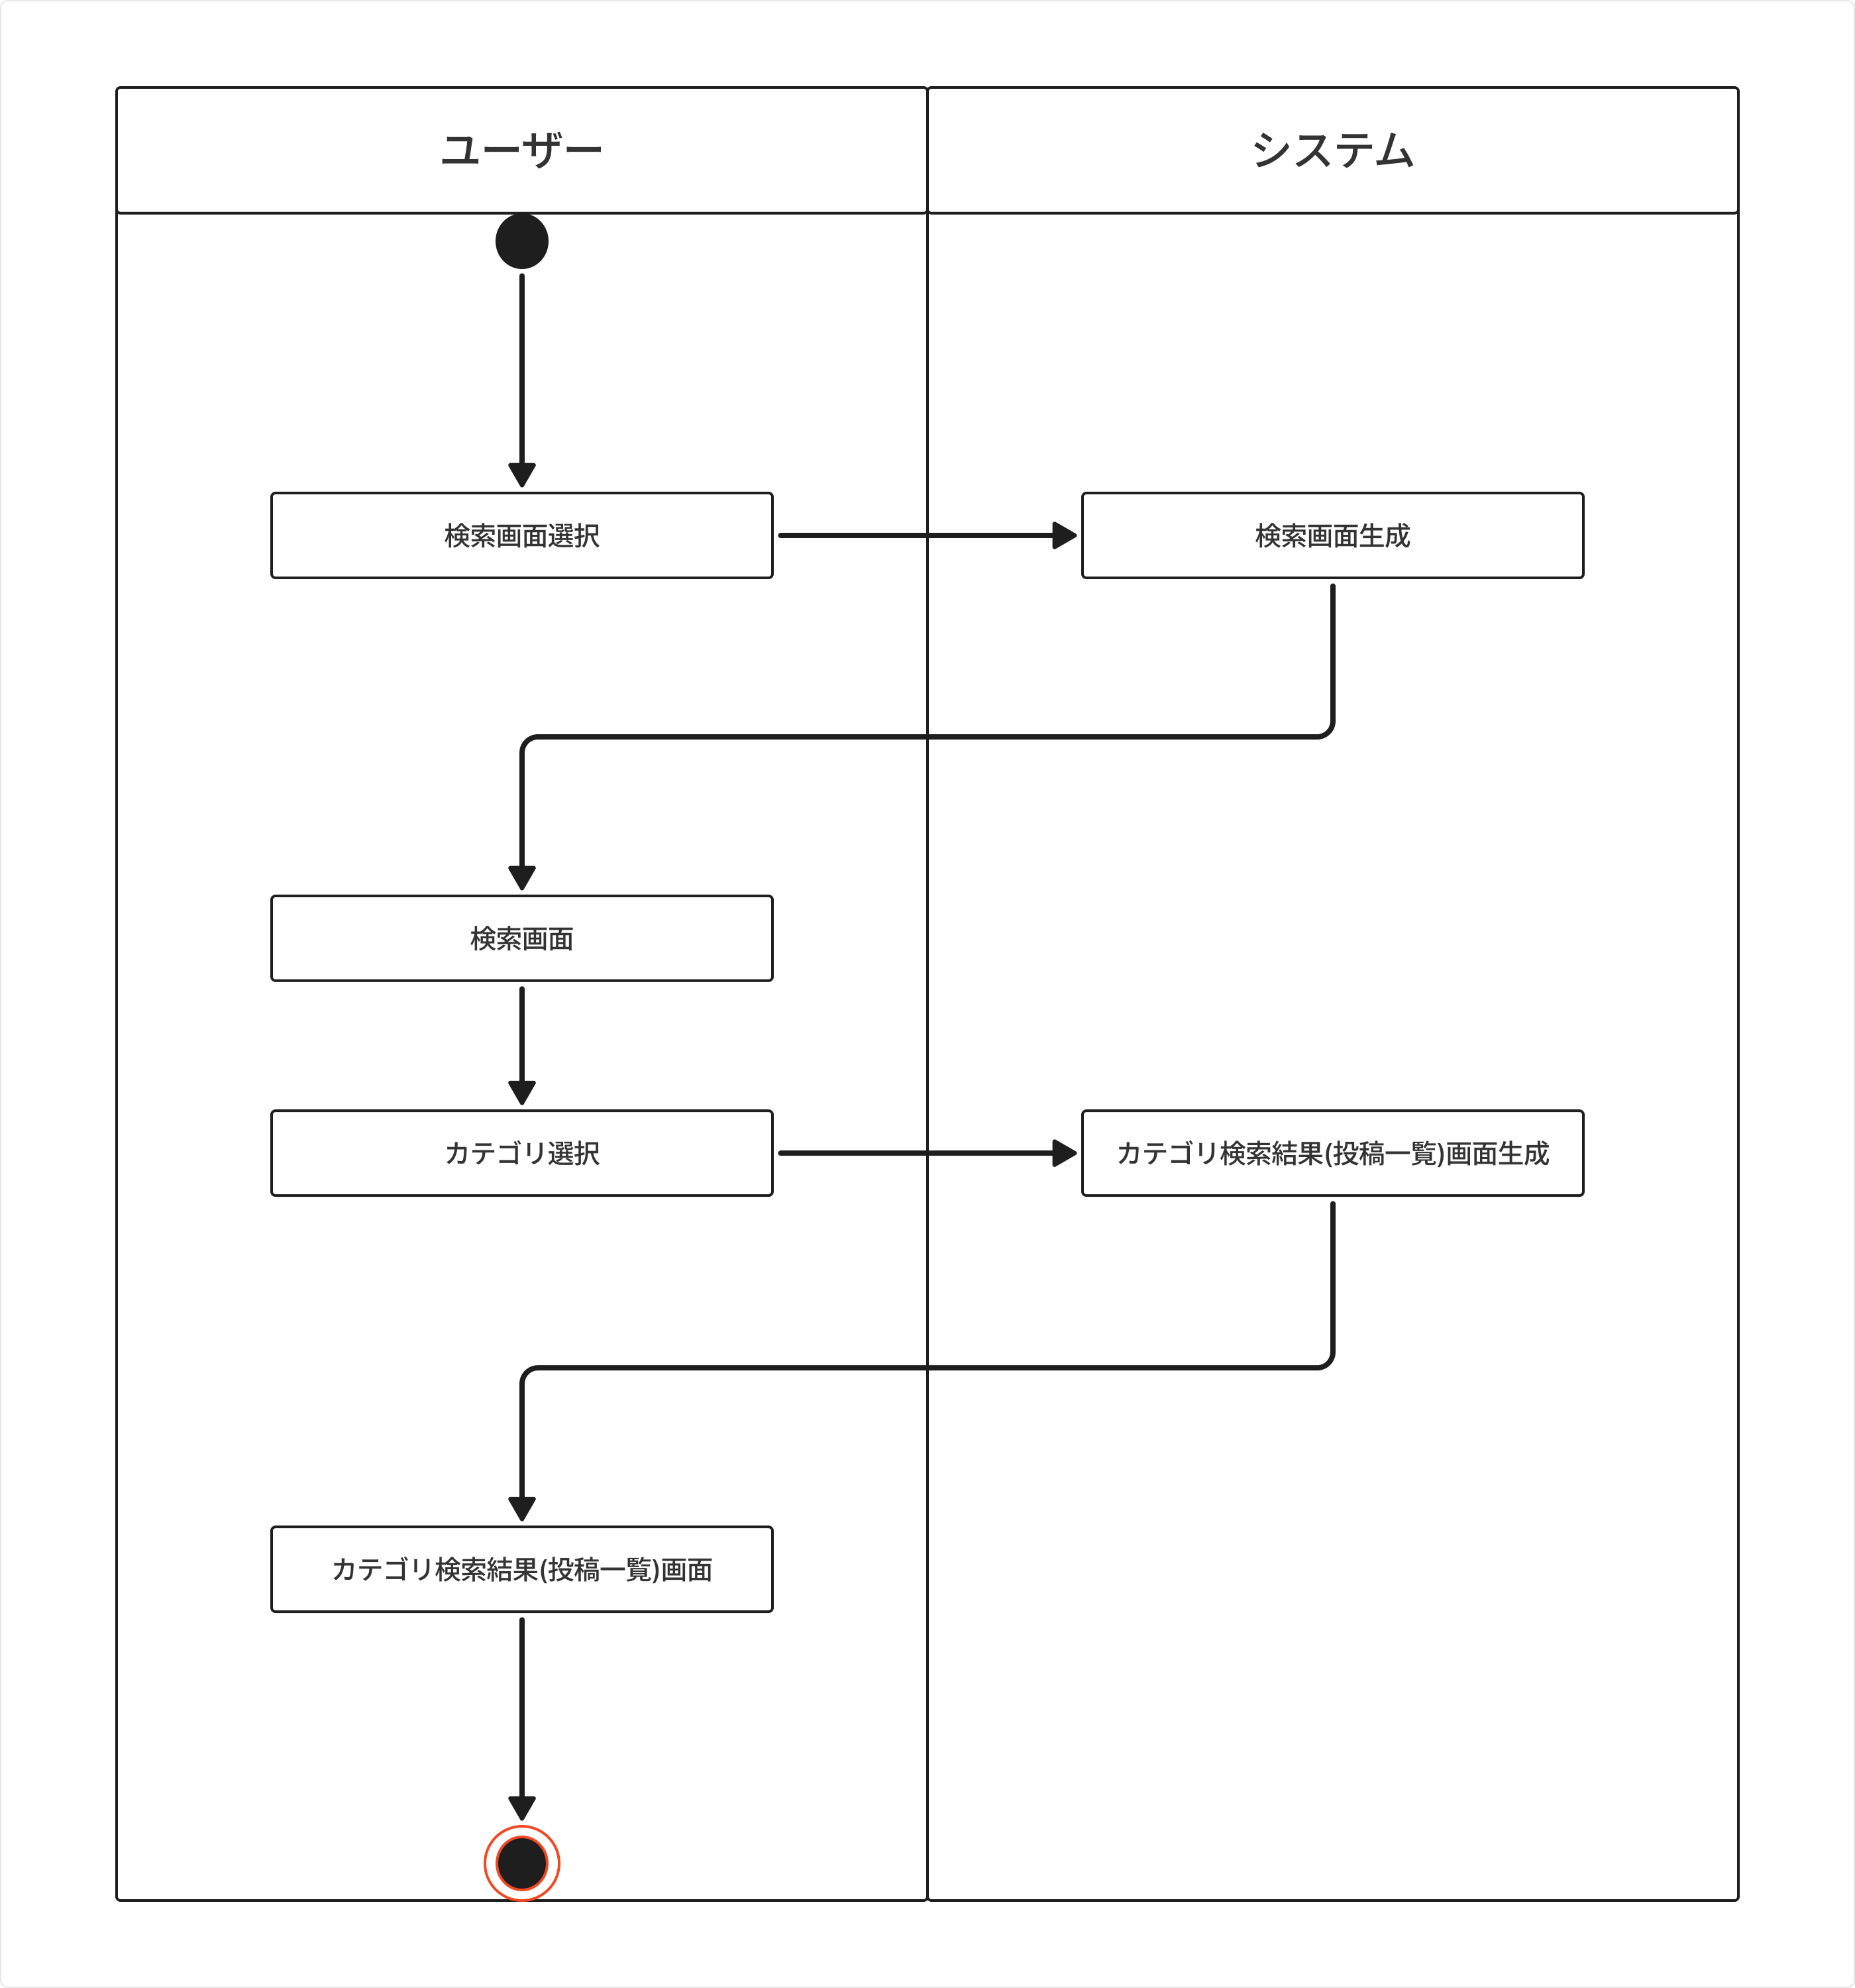
\includegraphics[width=\linewidth]{chapters/images/search_category.png}
    \caption{カテゴリ検索機能のアクティビティ図}
    \label{fig:search-category}
  \end{minipage}
\end{figure}

\begin{figure}[H]
  \centering
  \begin{minipage}[t]{0.35\linewidth}
    \centering
    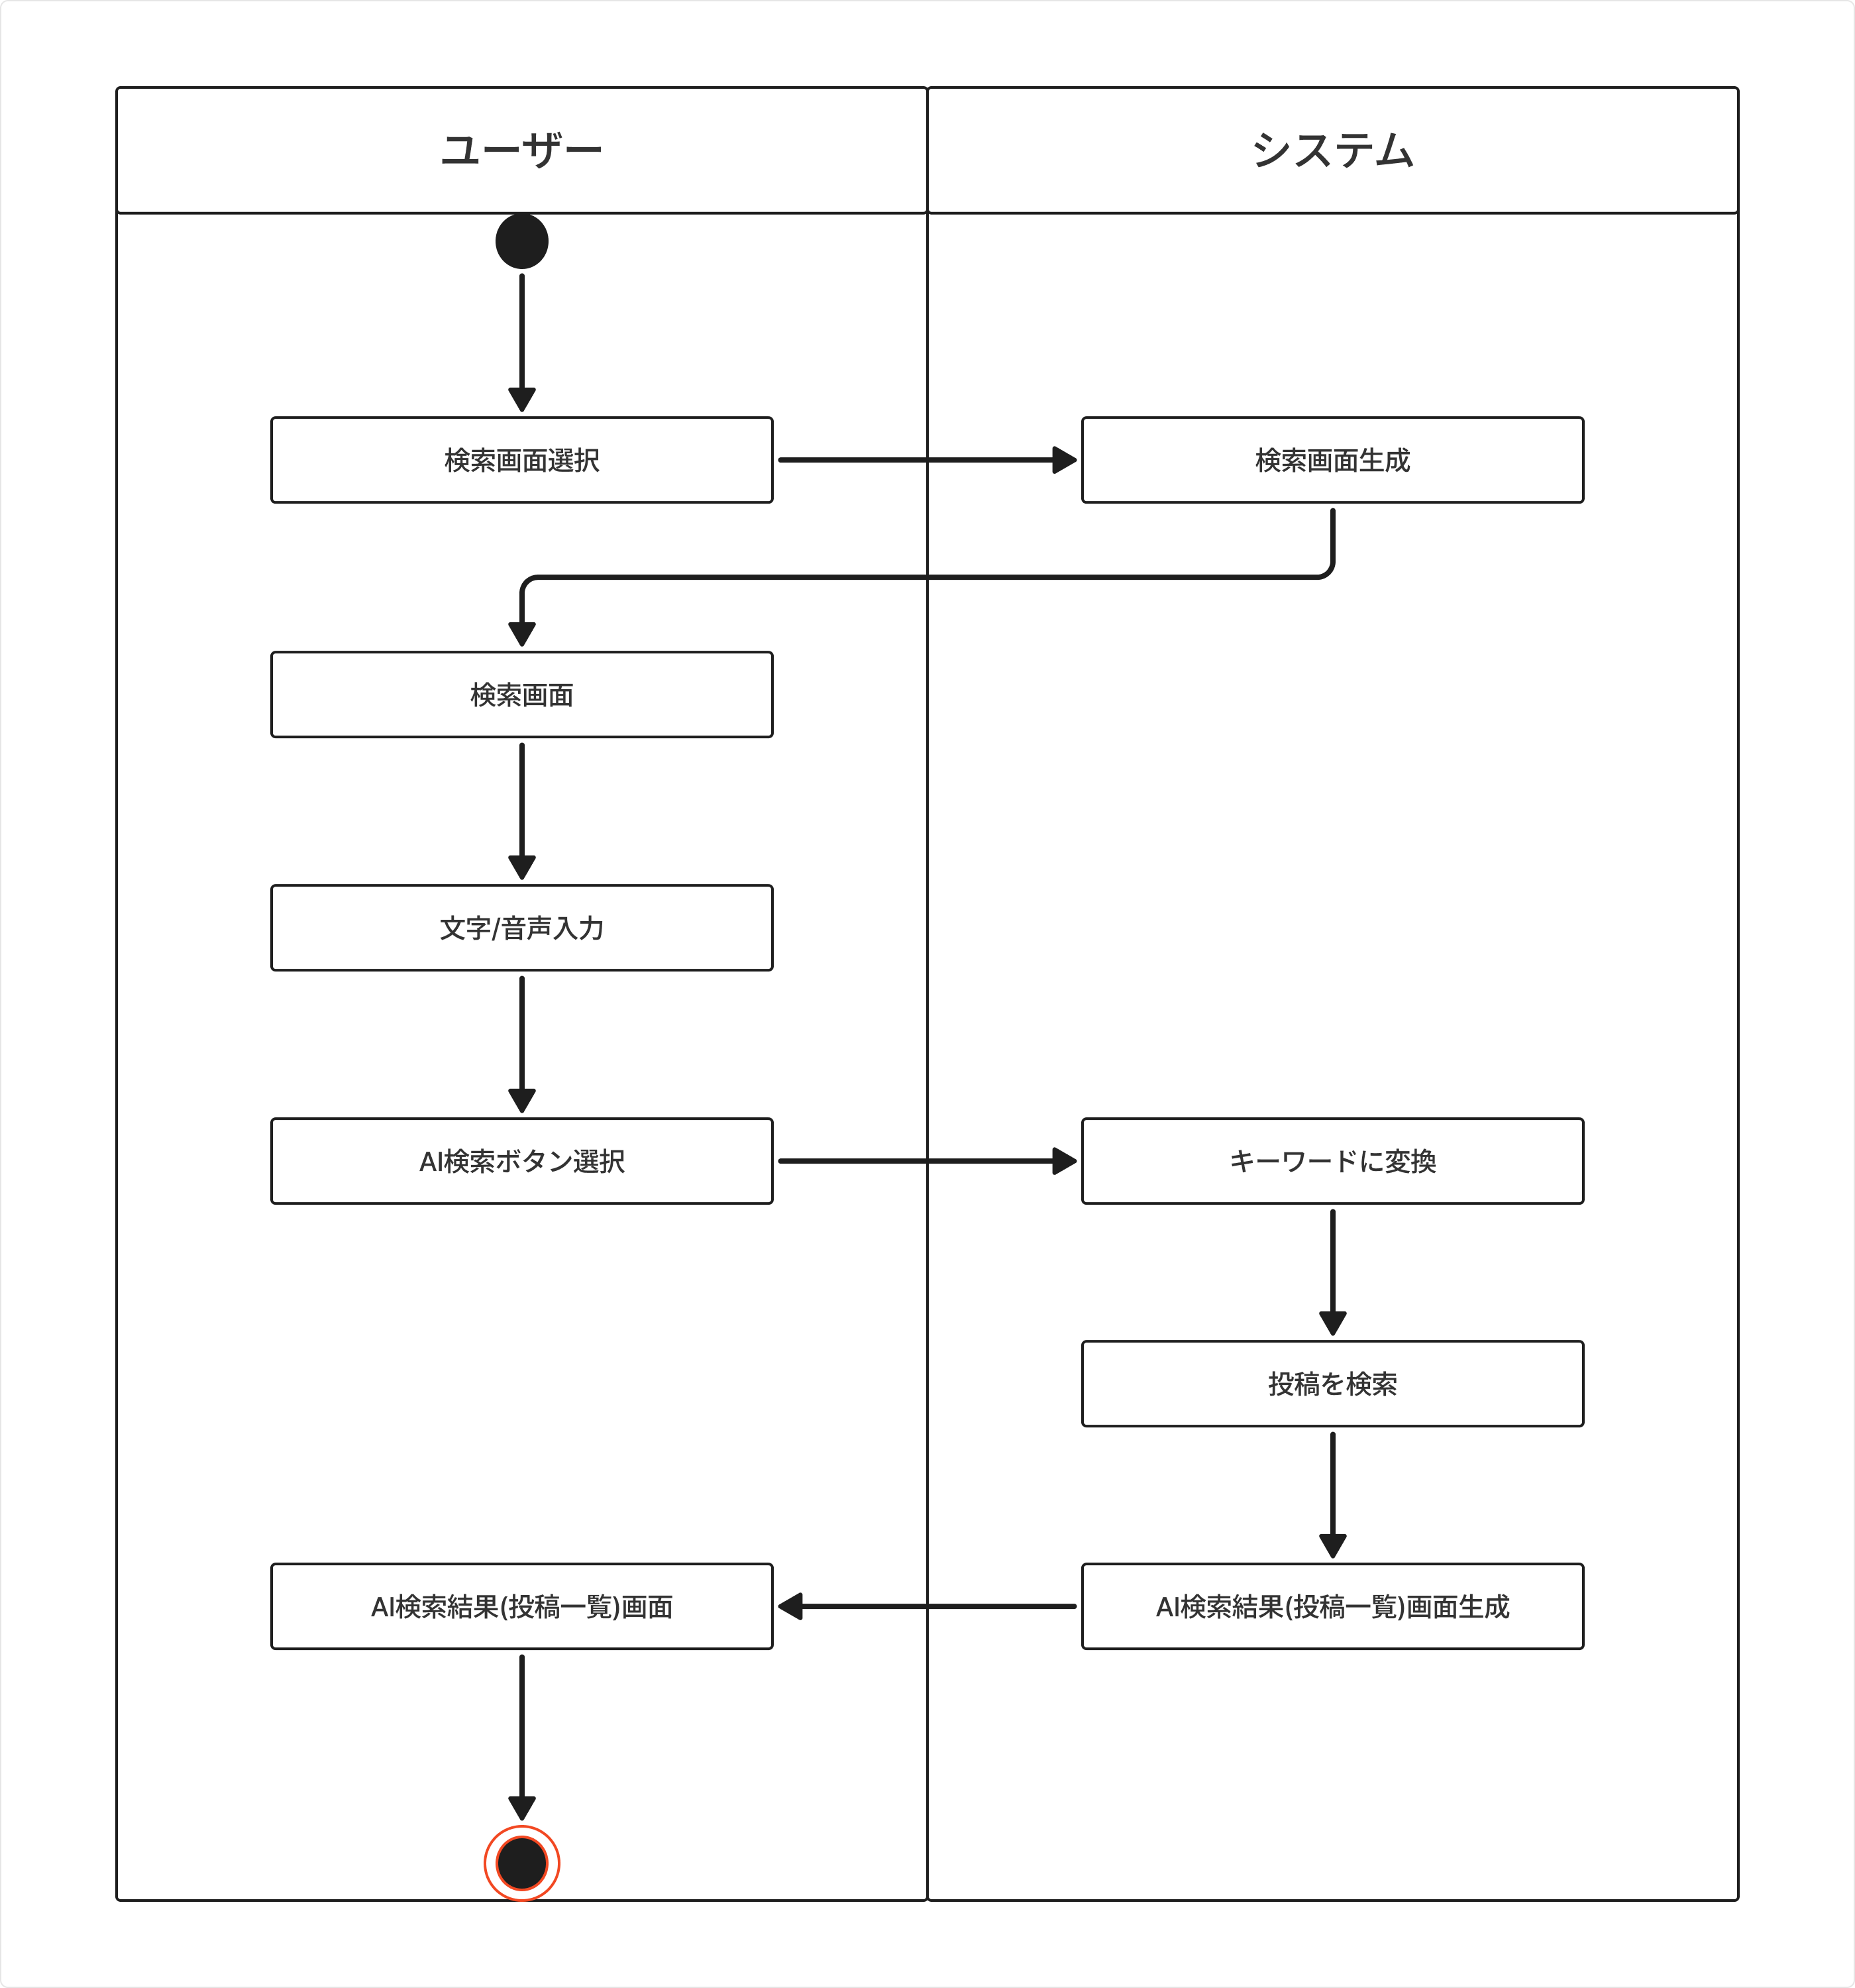
\includegraphics[width=\linewidth]{chapters/images/search_ai.png}
    \caption{AI検索機能のアクティビティ図}
    \label{fig:search-ai}
  \end{minipage}
  \hfill
  \begin{minipage}[t]{0.35\linewidth}
    \centering
    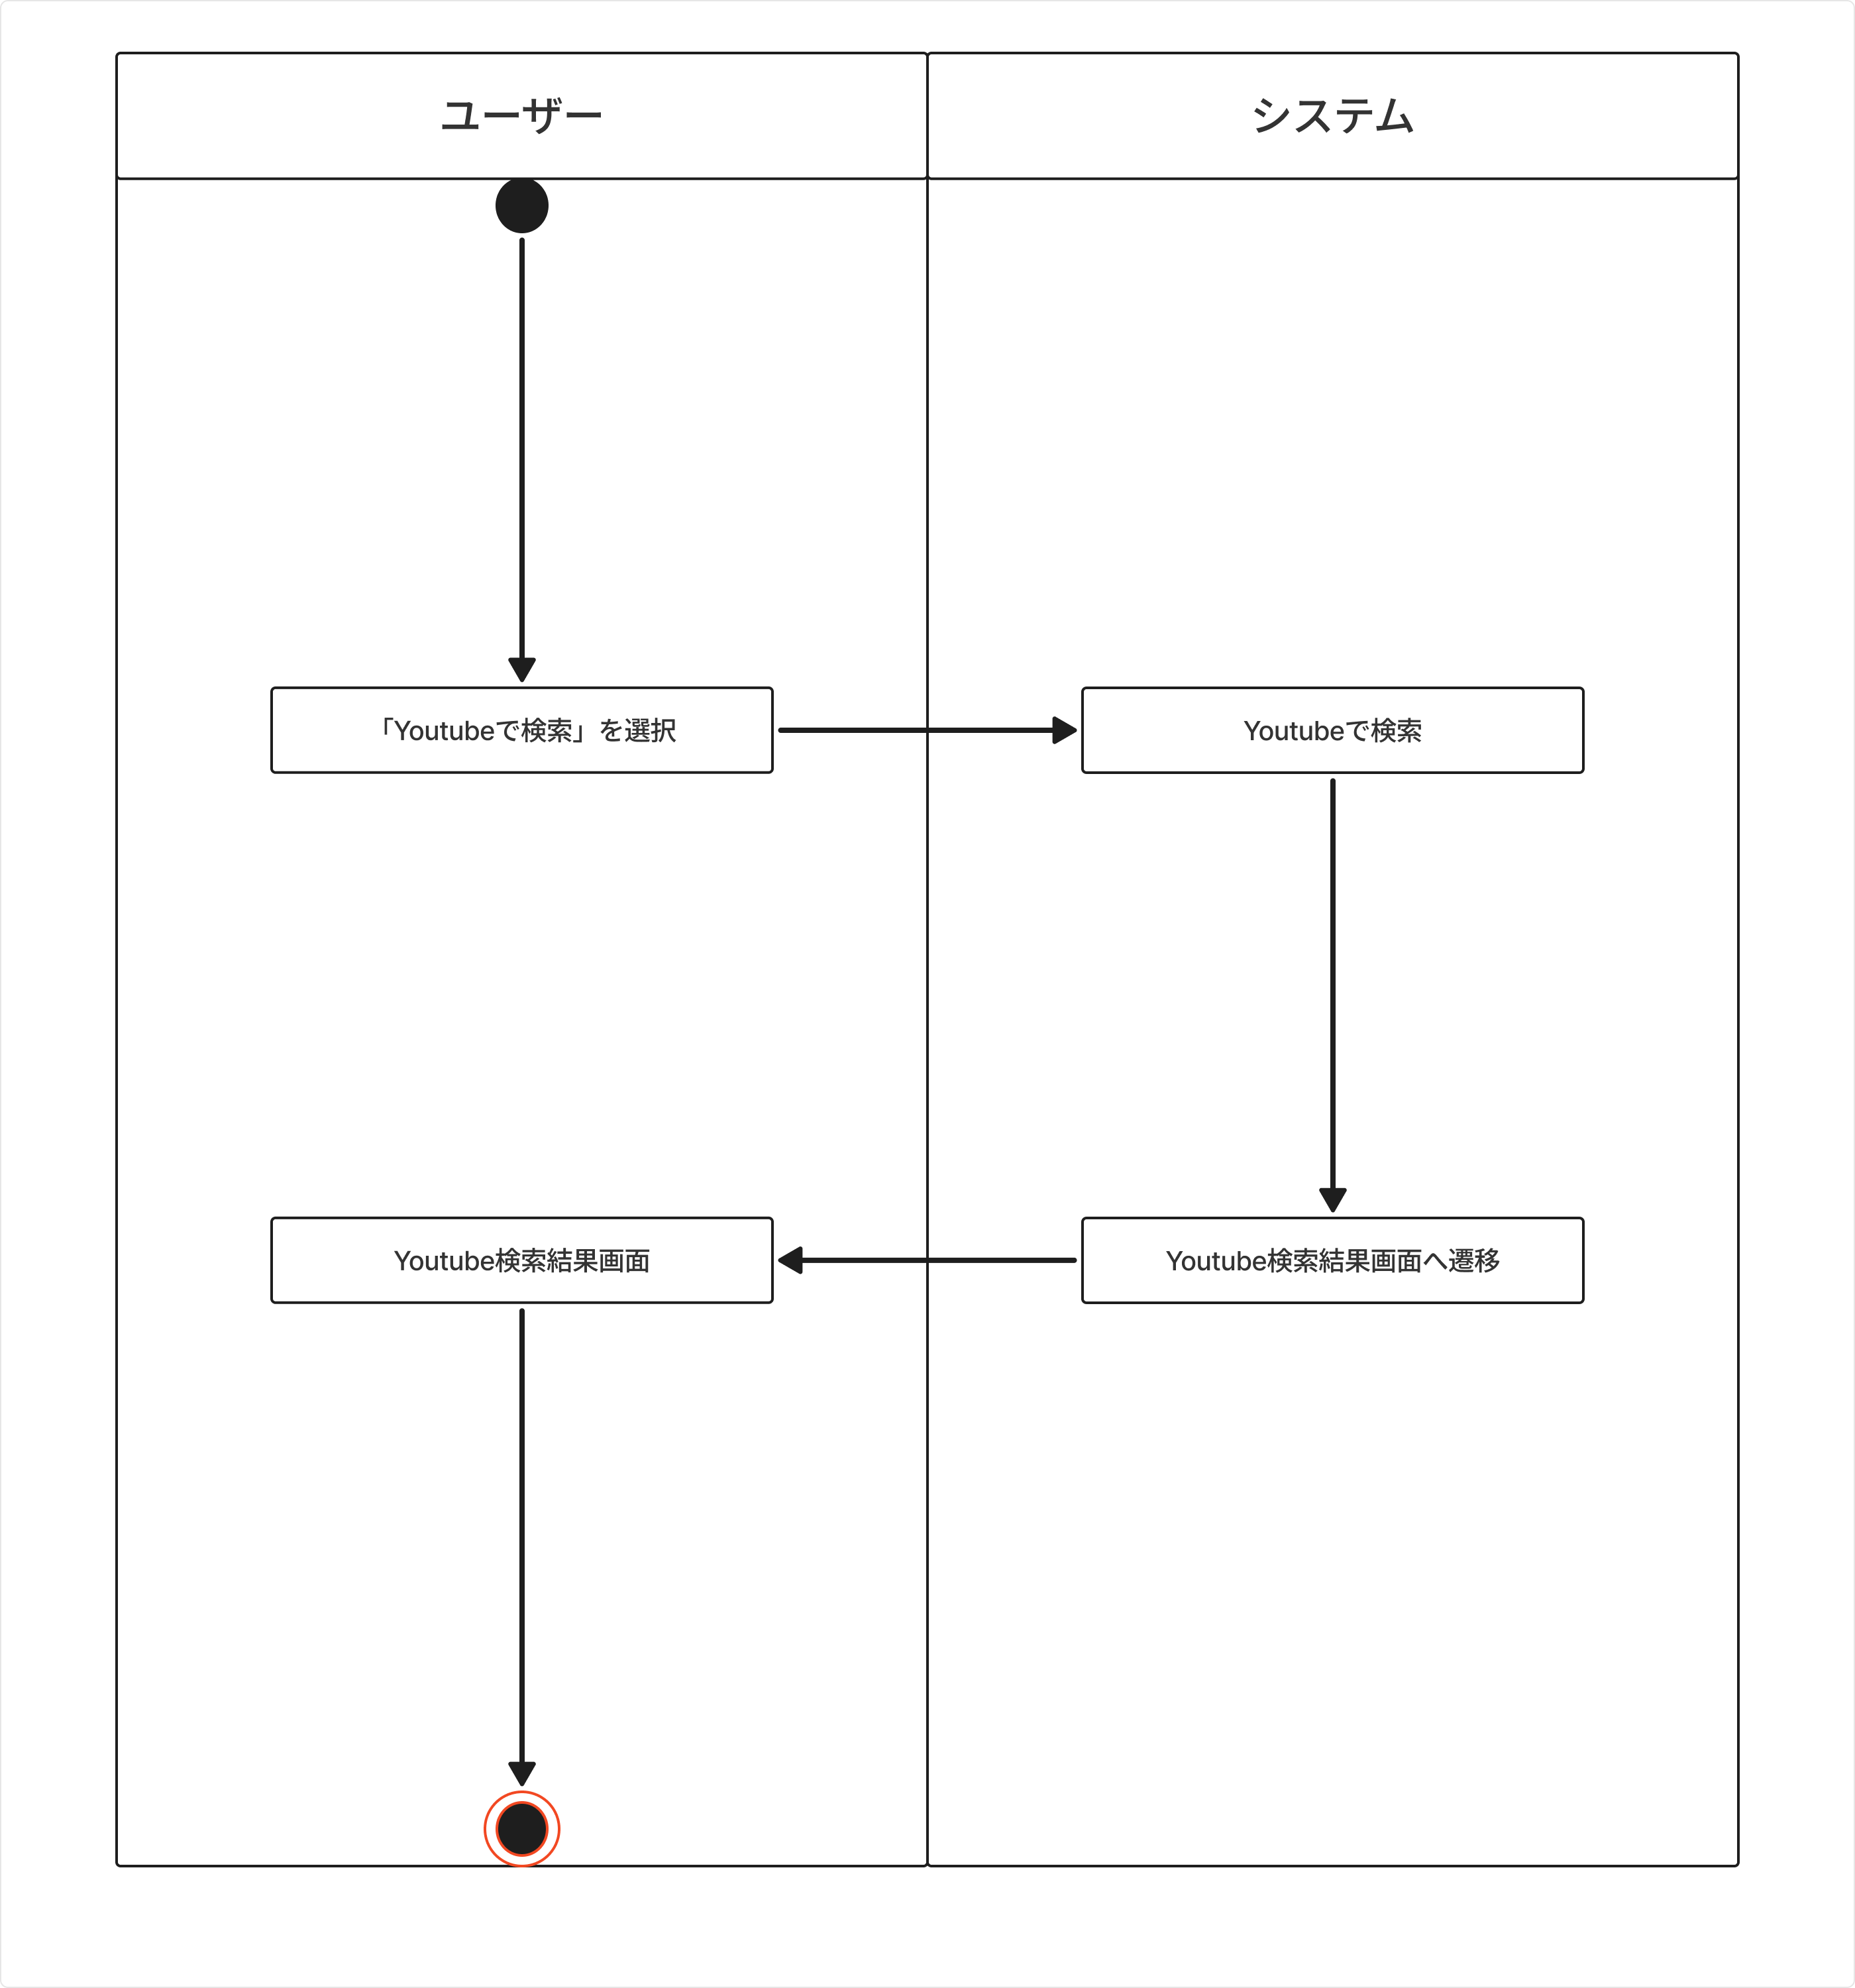
\includegraphics[width=\linewidth]{chapters/images/research_youtube.png}
    \caption{再検索機能のアクティビティ図}
    \label{fig:research}
  \end{minipage}
\end{figure}

%----------------------------------------------------------------------
\subsubsection{投稿閲覧機能}\label{subsec:post-view}
%----------------------------------------------------------------------
検索結果などの投稿を一覧で閲覧する機能である.
投稿一覧画面の上部にはAIレコメンド投稿を表示する.
投稿の並び順は「おすすめ」「ハートが多い順」「新着順」から選んで並べ替えることができる.
「おすすめ」はキーワードとの関連度が高い順であり, 検索結果を最初に表示するときの並び順とする.
一覧は上下のスワイプ操作で閲覧でき, 最後までスワイプすると, YouTubeで再検索する選択肢が表示される.

図\ref{fig:post-view}に投稿閲覧機能の流れを示す.

\begin{figure}[H]
  \centering
  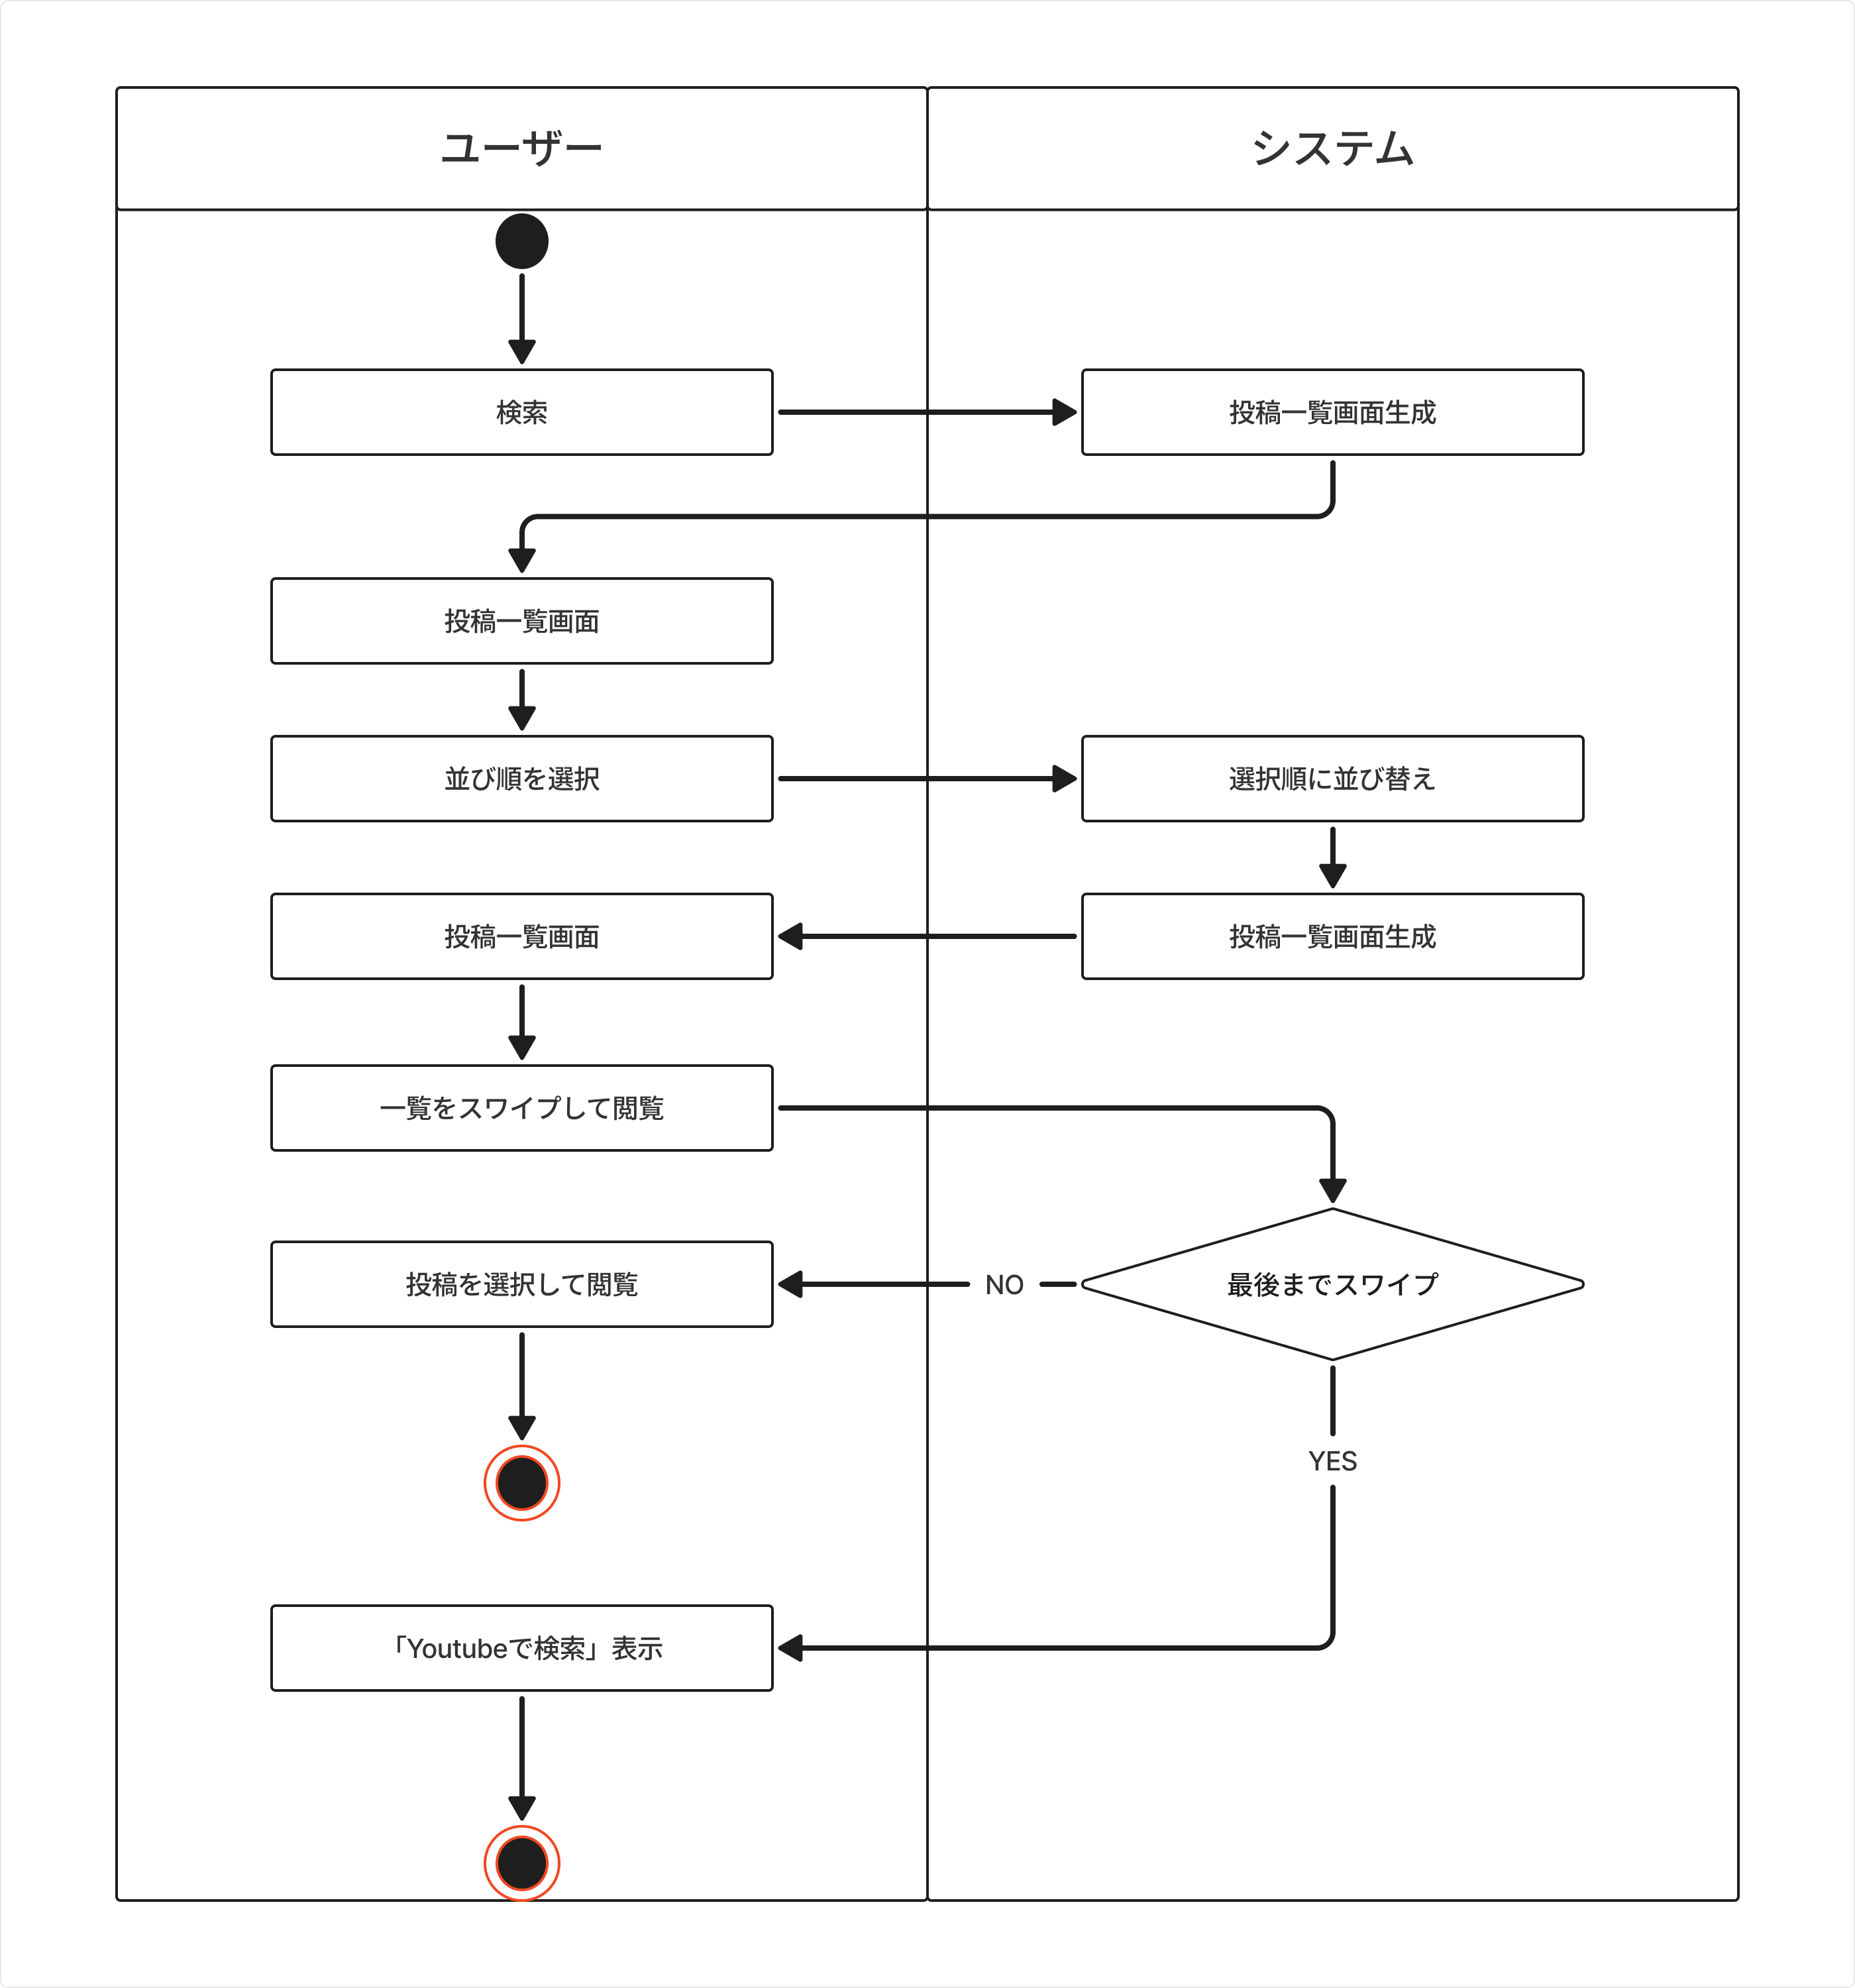
\includegraphics[width=0.6\linewidth]{chapters/images/post_view.png}
  \caption{投稿閲覧機能のアクティビティ図}
  \label{fig:post-view}
\end{figure}

%----------------------------------------------------------------------
\subsubsection{投稿通報機能}\label{subsec:report}
%----------------------------------------------------------------------
閲覧中の投稿に誤情報や不適切な内容が含まれている場合に, 運営へ通報する機能である.
利用者は, 投稿の下部に「♥」ボタンと並んで表示される通報ボタンを押し, 通報理由を選択して詳しい内容を記述する.
通報された投稿は, 管理者が内容を確認して対応する.

図\ref{fig:report}に投稿通報機能の流れを示す.

\begin{figure}[H]
  \centering
  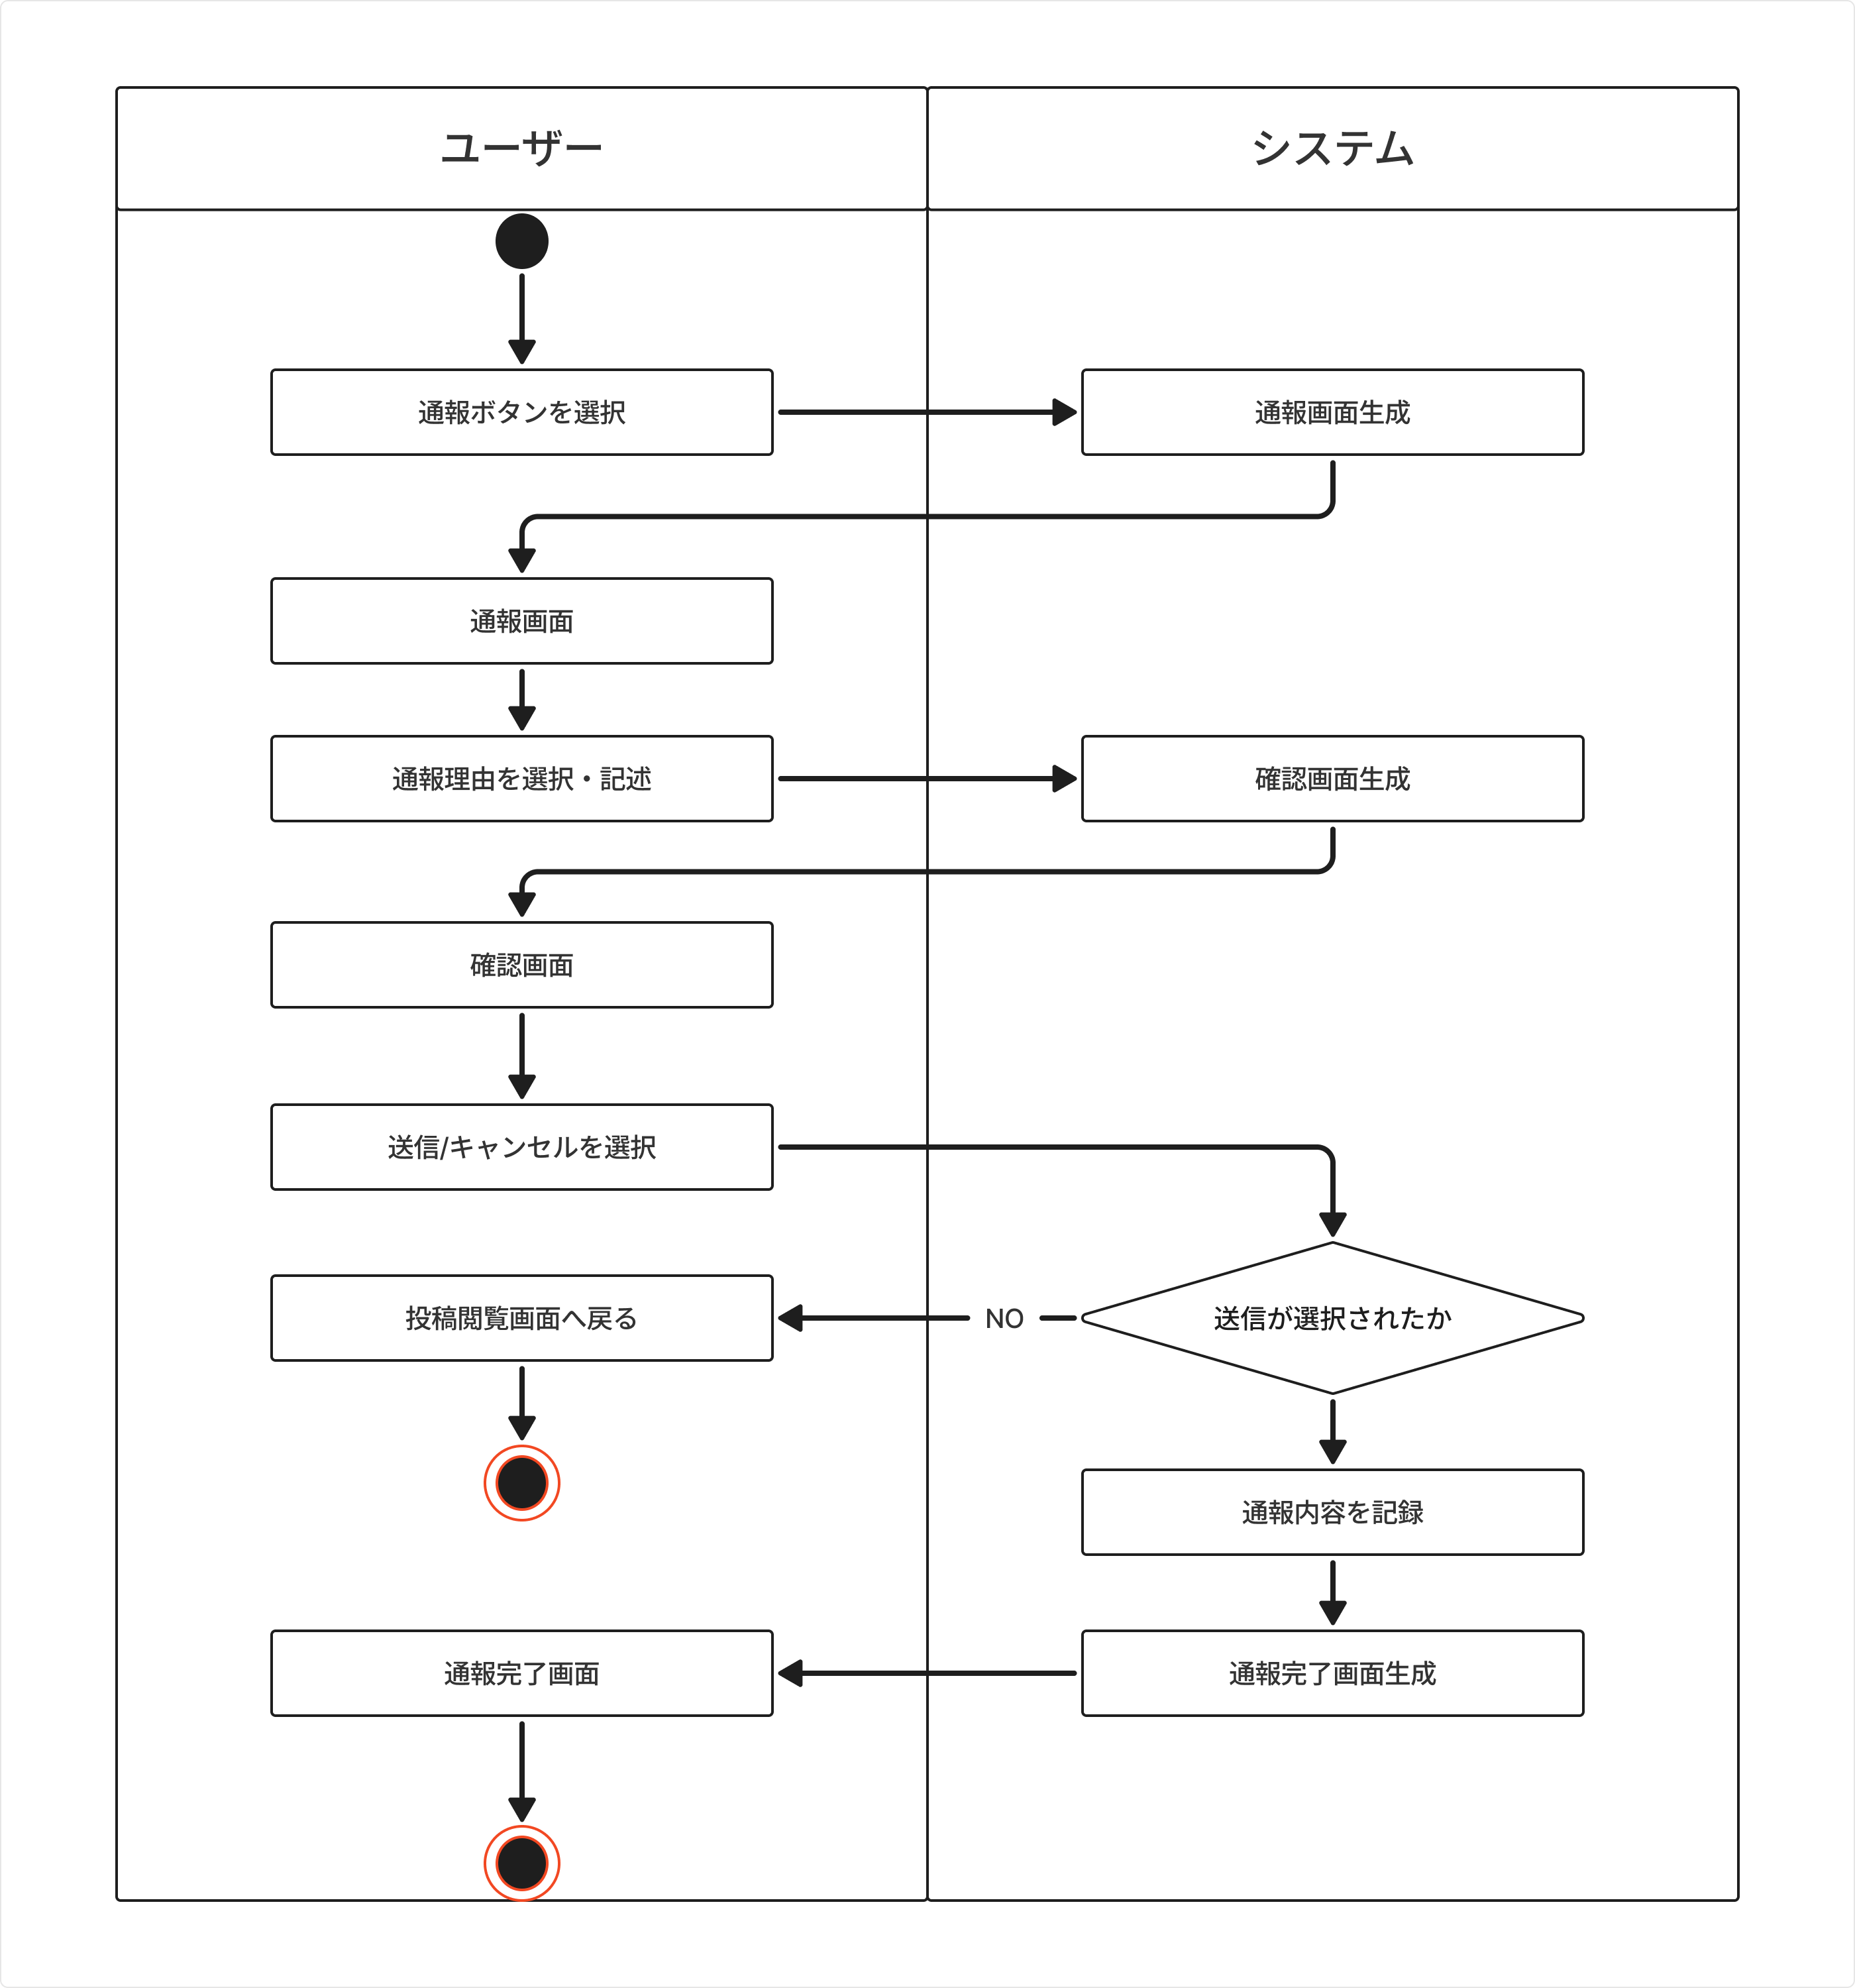
\includegraphics[width=0.6\linewidth]{chapters/images/report.png}
  \caption{投稿通報機能のアクティビティ図}
  \label{fig:report}
\end{figure}

%----------------------------------------------------------------------
\subsubsection{設定機能}\label{subsec:settings}
%----------------------------------------------------------------------
利用者が, 画面表示・操作支援および通知に関する設定を行う機能である.
設定できる項目を表\ref{tab:settings}に示す.

\begin{table}[H]
  \centering
  \caption{設定項目}
  \label{tab:settings}
  \begin{tabular}{ll}
    \hline
    画面表示・操作支援 & 文字・ボタンの大きさ \\
                       & 画面の配色 \\
                       & AI音声の読み上げ \\
                       & アプリ内の音量 \\
    \hline
    通知設定           & アプリからの通知を受け取るかどうか \\
    \hline
  \end{tabular}
\end{table}

図\ref{fig:act-settings}に設定機能の流れを示す.

\begin{figure}[H]
  \centering
  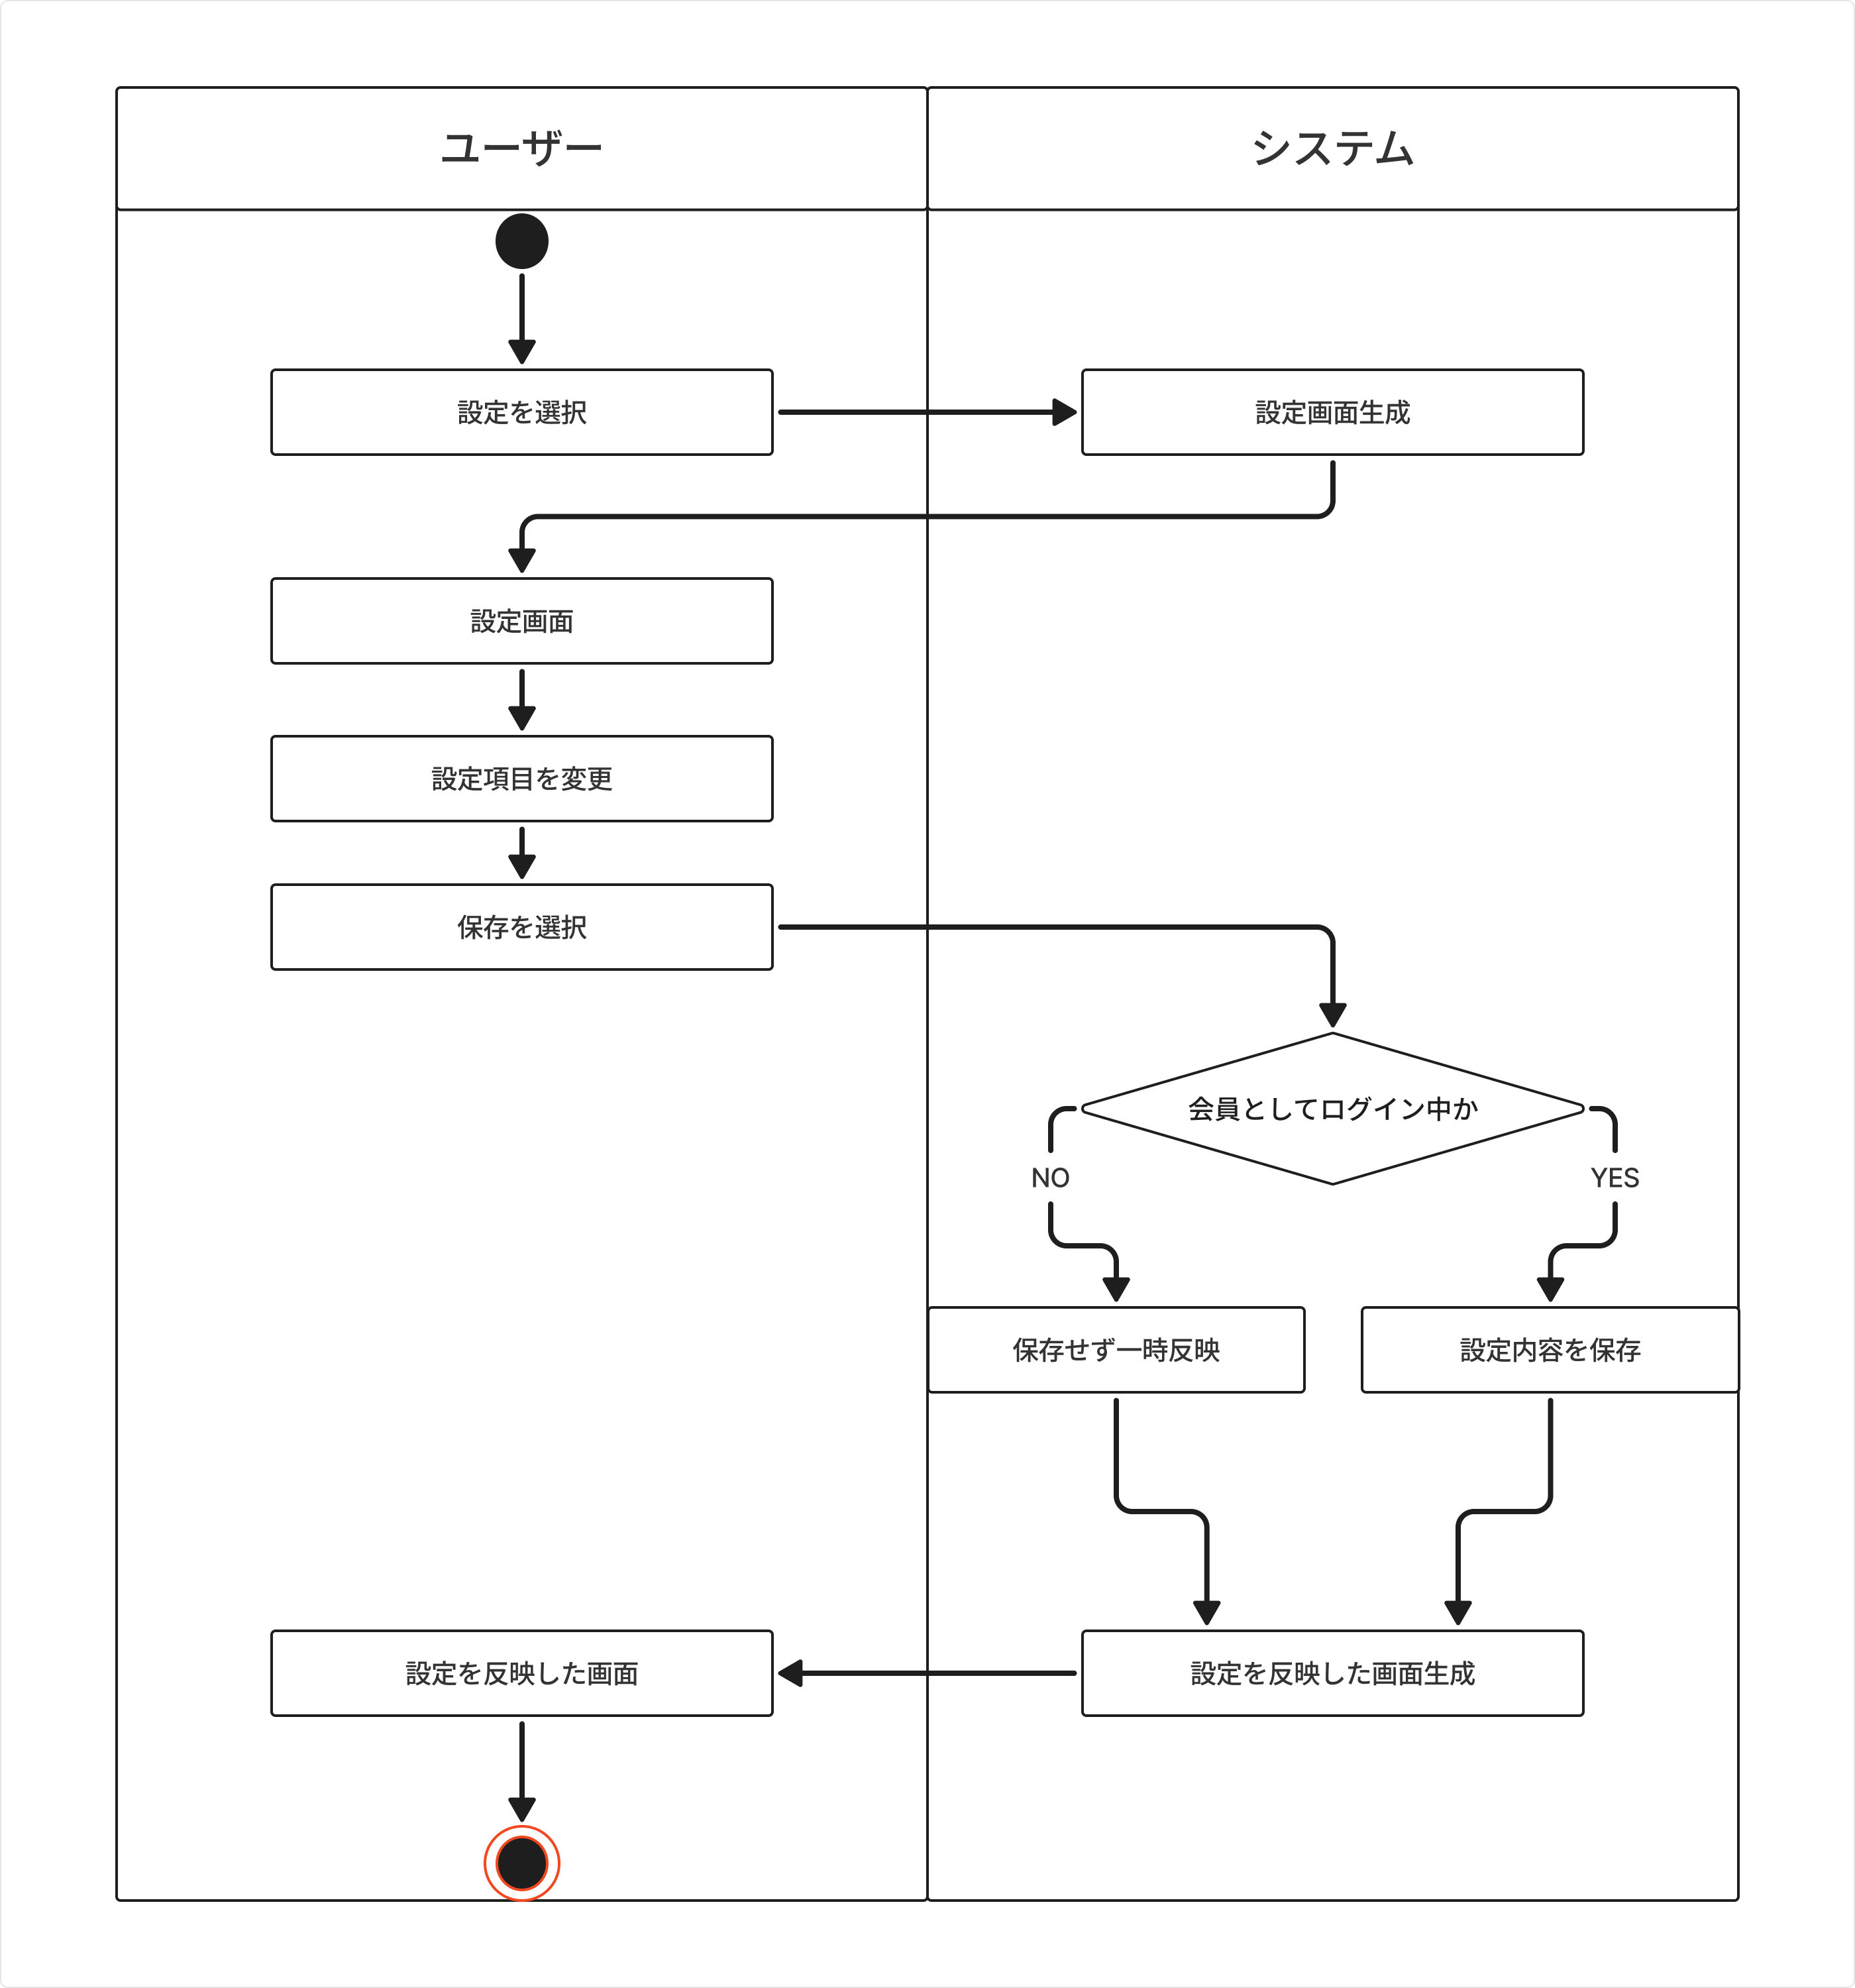
\includegraphics[width=0.5\linewidth]{chapters/images/settings.png}
  \caption{設定機能のアクティビティ図}
  \label{fig:act-settings}
\end{figure}

%----------------------------------------------------------------------
\subsubsection{問い合わせ機能}\label{subsec:inquiry}
%----------------------------------------------------------------------
利用者が、運営にメッセージで問い合わせる機能である.
送信された内容は, 管理者が確認して対応する.

図\ref{fig:inquiry}に問い合わせ機能の流れを示す.

\begin{figure}[H]
  \centering
  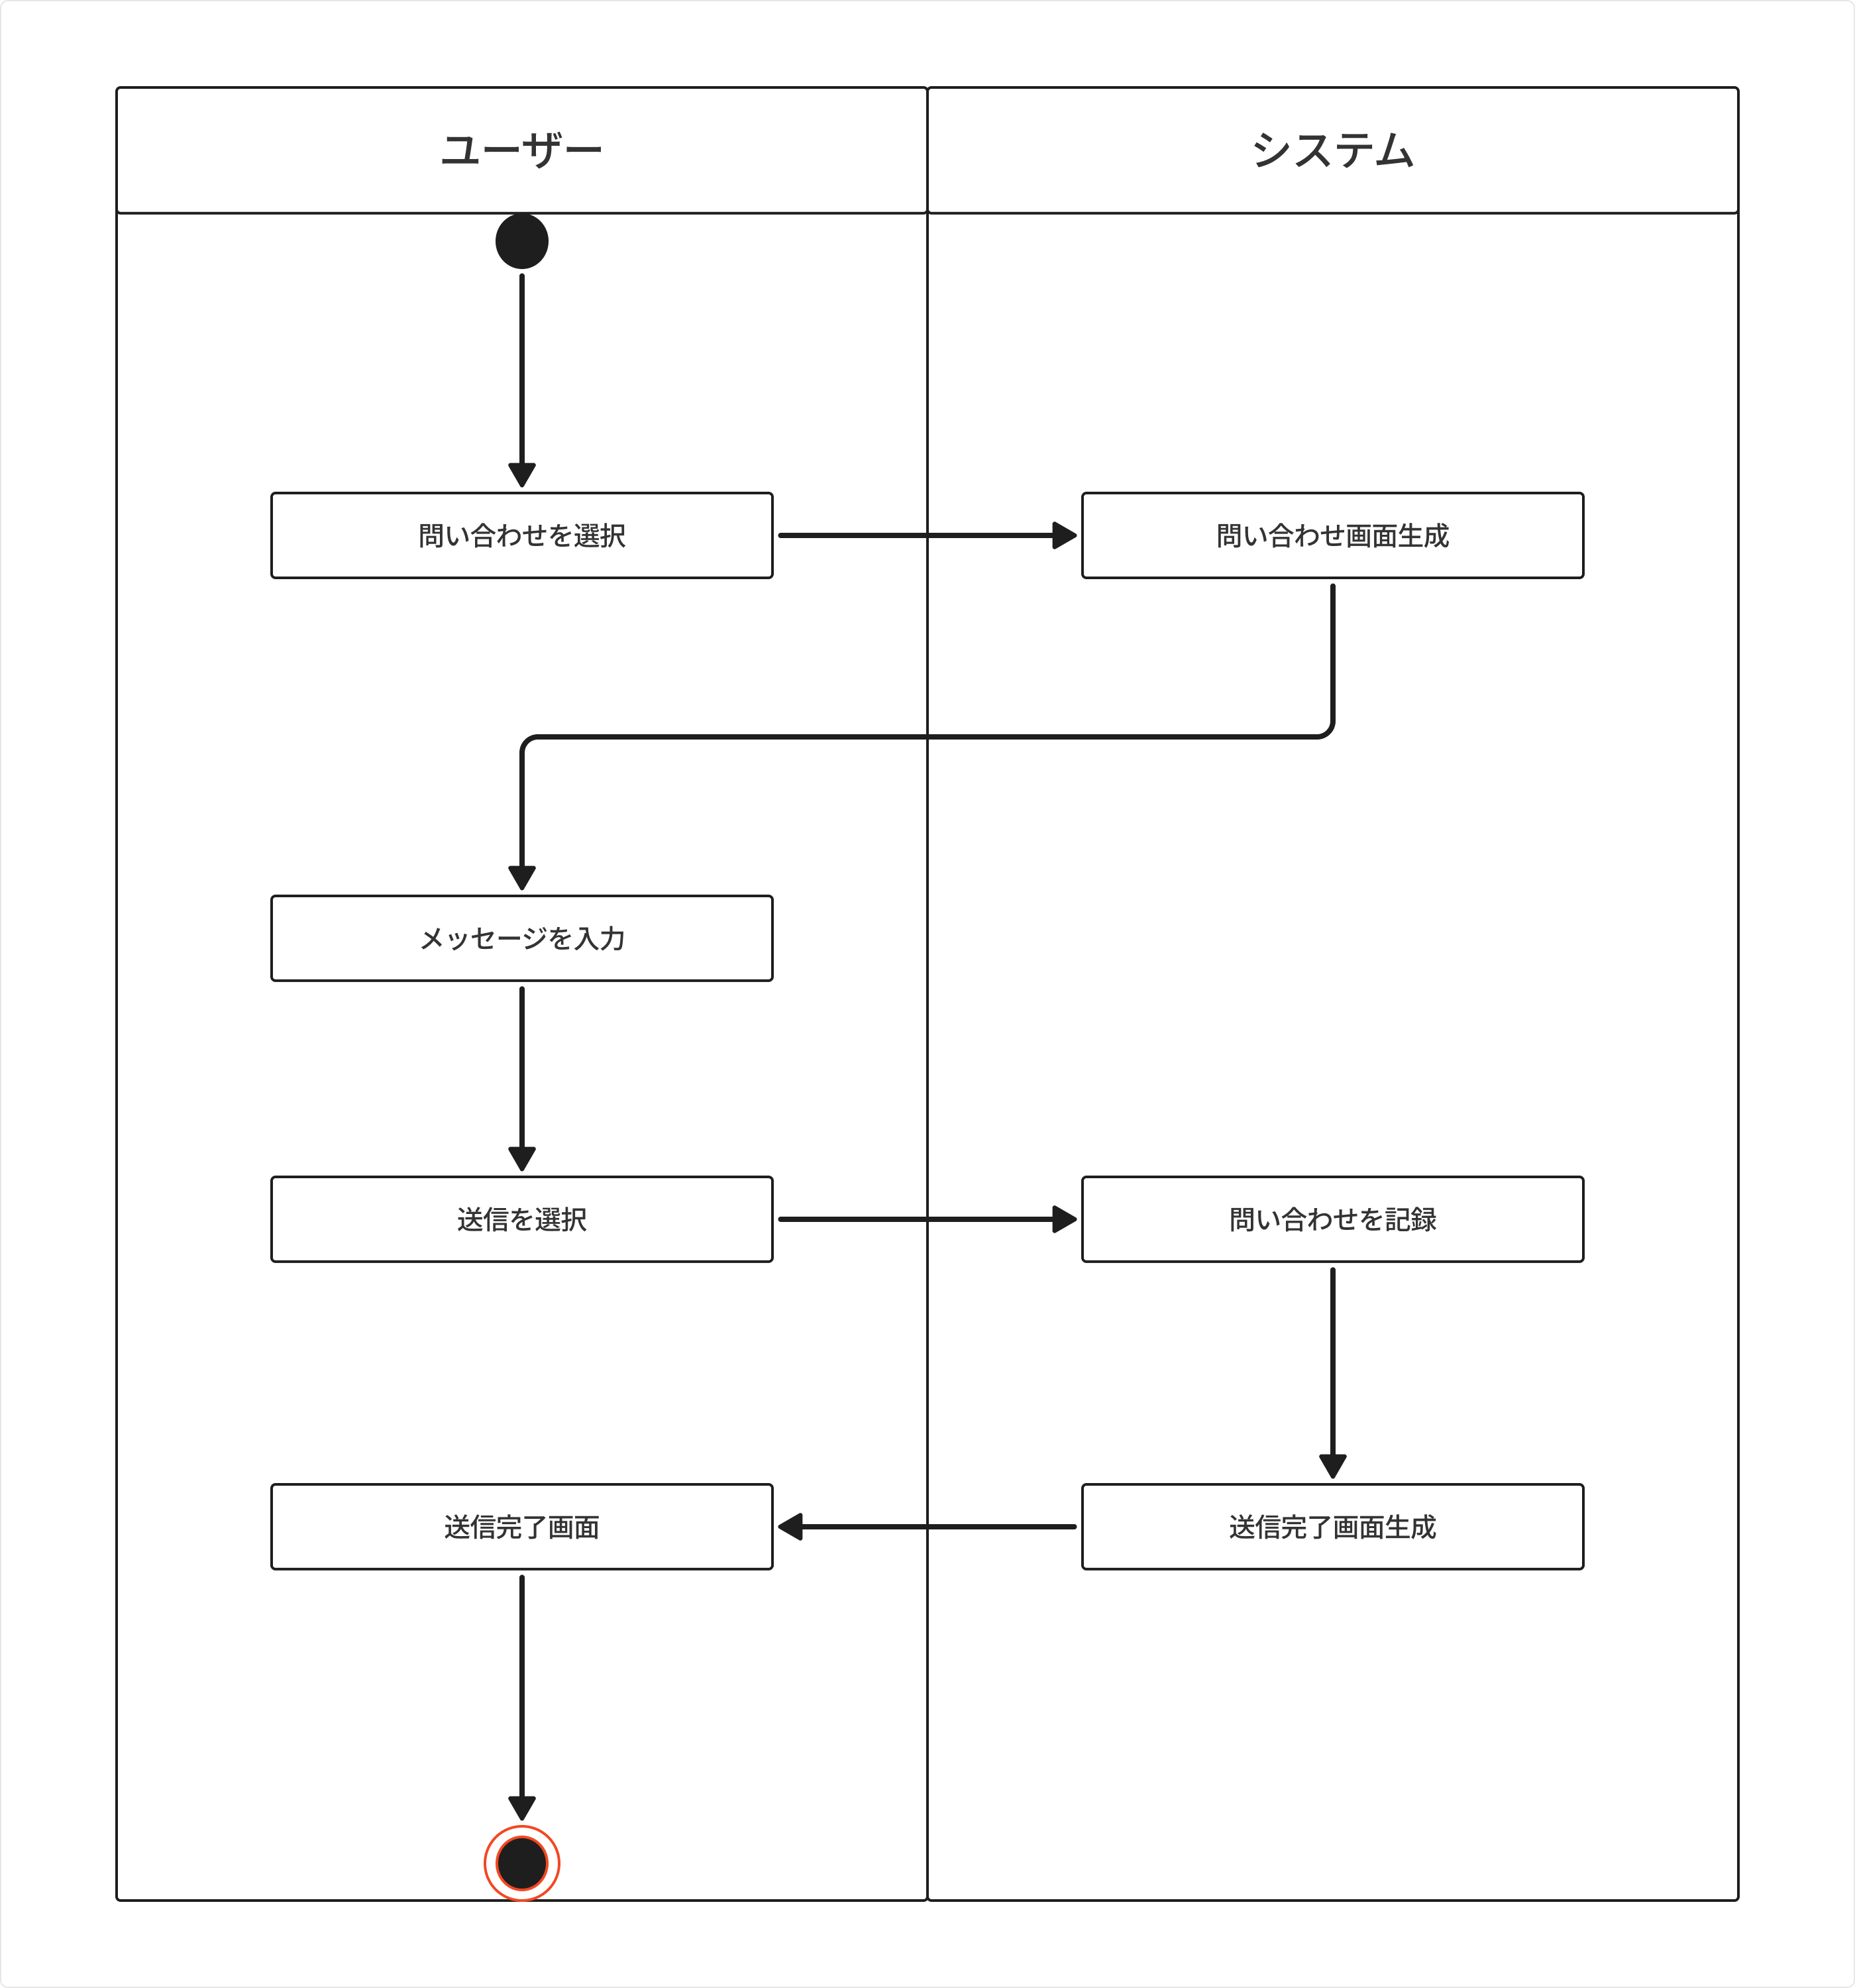
\includegraphics[width=0.5\linewidth]{chapters/images/inquiry.png}
  \caption{問い合わせ機能のアクティビティ図}
  \label{fig:inquiry}
\end{figure}

%----------------------------------------------------------------------
\subsubsection{タイアップ表示機能}\label{subsec:tieup}
%----------------------------------------------------------------------
協力企業などとのタイアップによる投稿を, 通常の投稿と同じ形式で表示する機能である.
タイアップの投稿には「PR」の文字を表示し, 通常の投稿と区別できるようにする.

\subsection{会員共通機能}\label{subsec:member}
%----------------------------------------------------------------------
本項では, 会員ユーザ（投稿者・学習者）に共通する機能について述べる.
各機能の処理の流れは, ユーザとシステムの2つのレーンに分けたアクティビティ図で示す.

%......................................................................
\subsubsection{新規会員登録機能}\label{subsubsec:register}
%......................................................................
新規利用者の会員登録を行う機能である.
初期画面で「新規会員登録」を選択し, 利用目的を選んで利用規約に同意したあと, 6つのステップで登録情報を入力する.
入力する項目は, 氏名, ニックネーム, 性別, 生年月日, 携帯電話番号である.
電話番号は, ショートメッセージ（SMS）で届く6桁の数字を入力することで確認する.
パスワードはシステムが自動で発行し, 利用者がそれを保管したことを確認してから登録を完了する.

処理の流れを図\ref{fig:register1}--\ref{fig:register3}に示す.
図中の丸囲みの「A」「B」は結合子であり, 次の図の同じ記号へ処理が続くことを表す.

\begin{figure}[H]
  \centering
  \begin{minipage}[t]{0.48\linewidth}
    \centering
    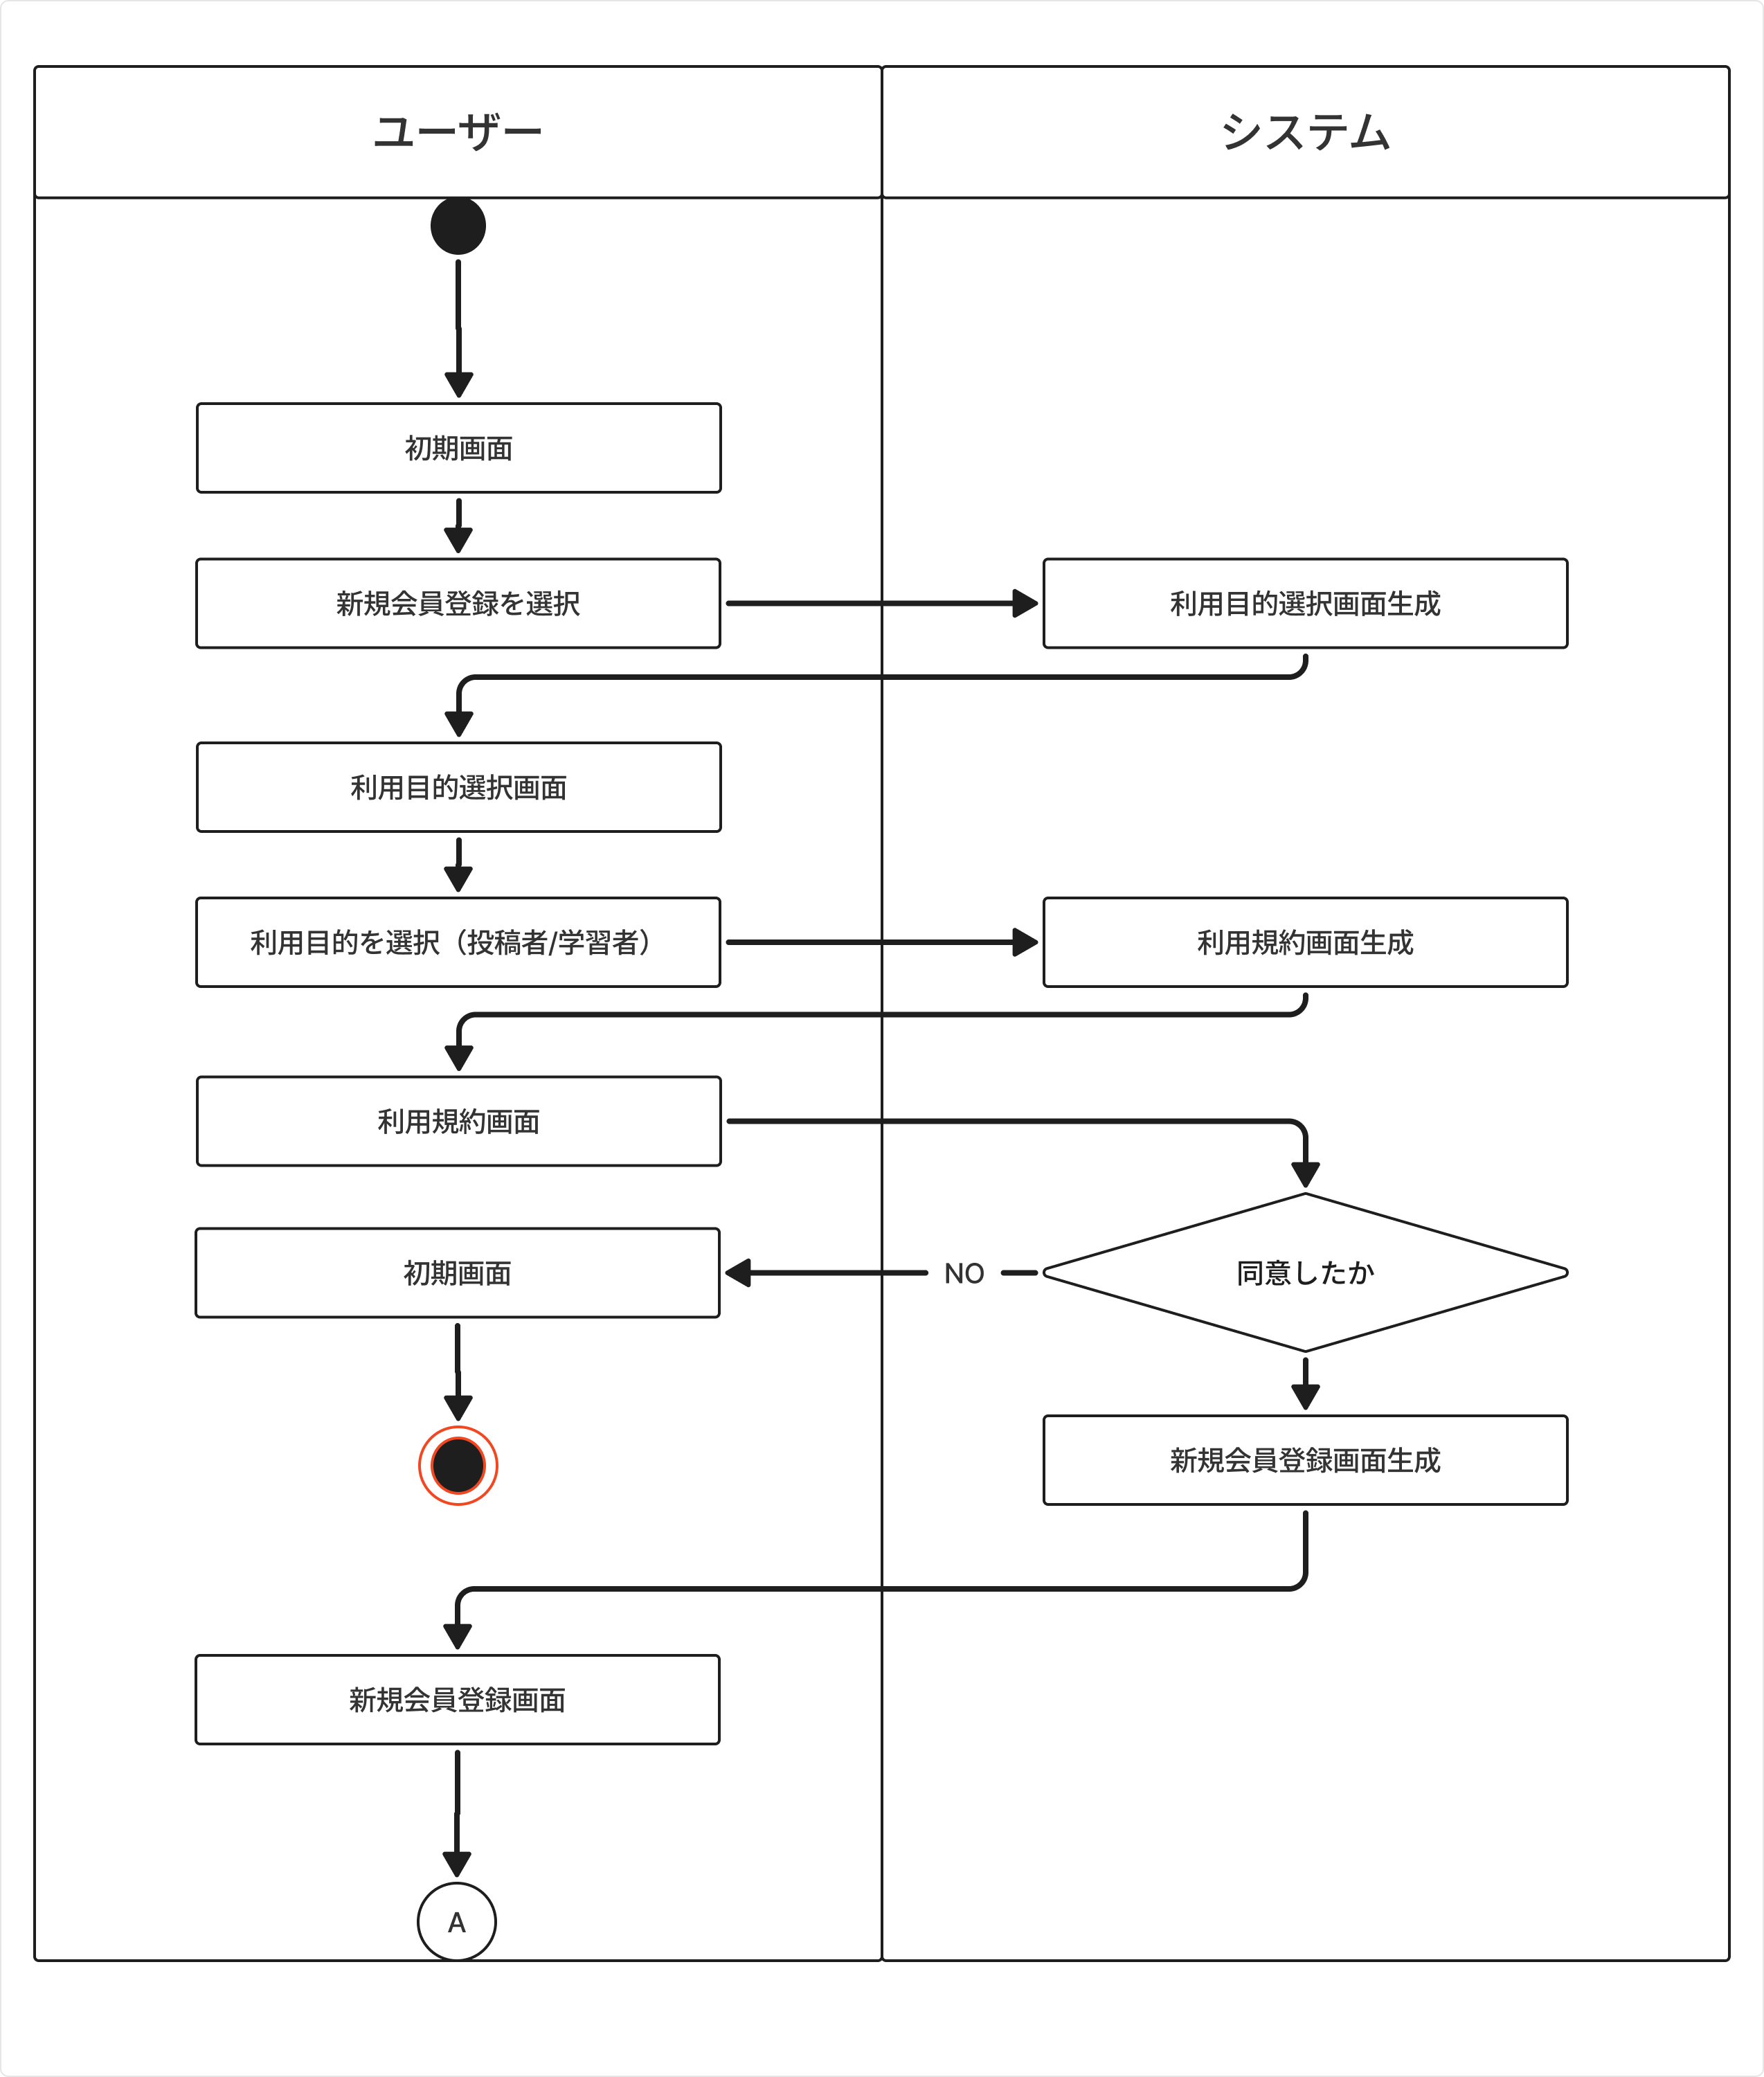
\includegraphics[width=\linewidth]{chapters/images/register1.png}
    \caption{新規会員登録機能のアクティビティ図1（利用目的・利用規約）}
    \label{fig:register1}
  \end{minipage}
  \hfill
  \begin{minipage}[t]{0.48\linewidth}
    \centering
    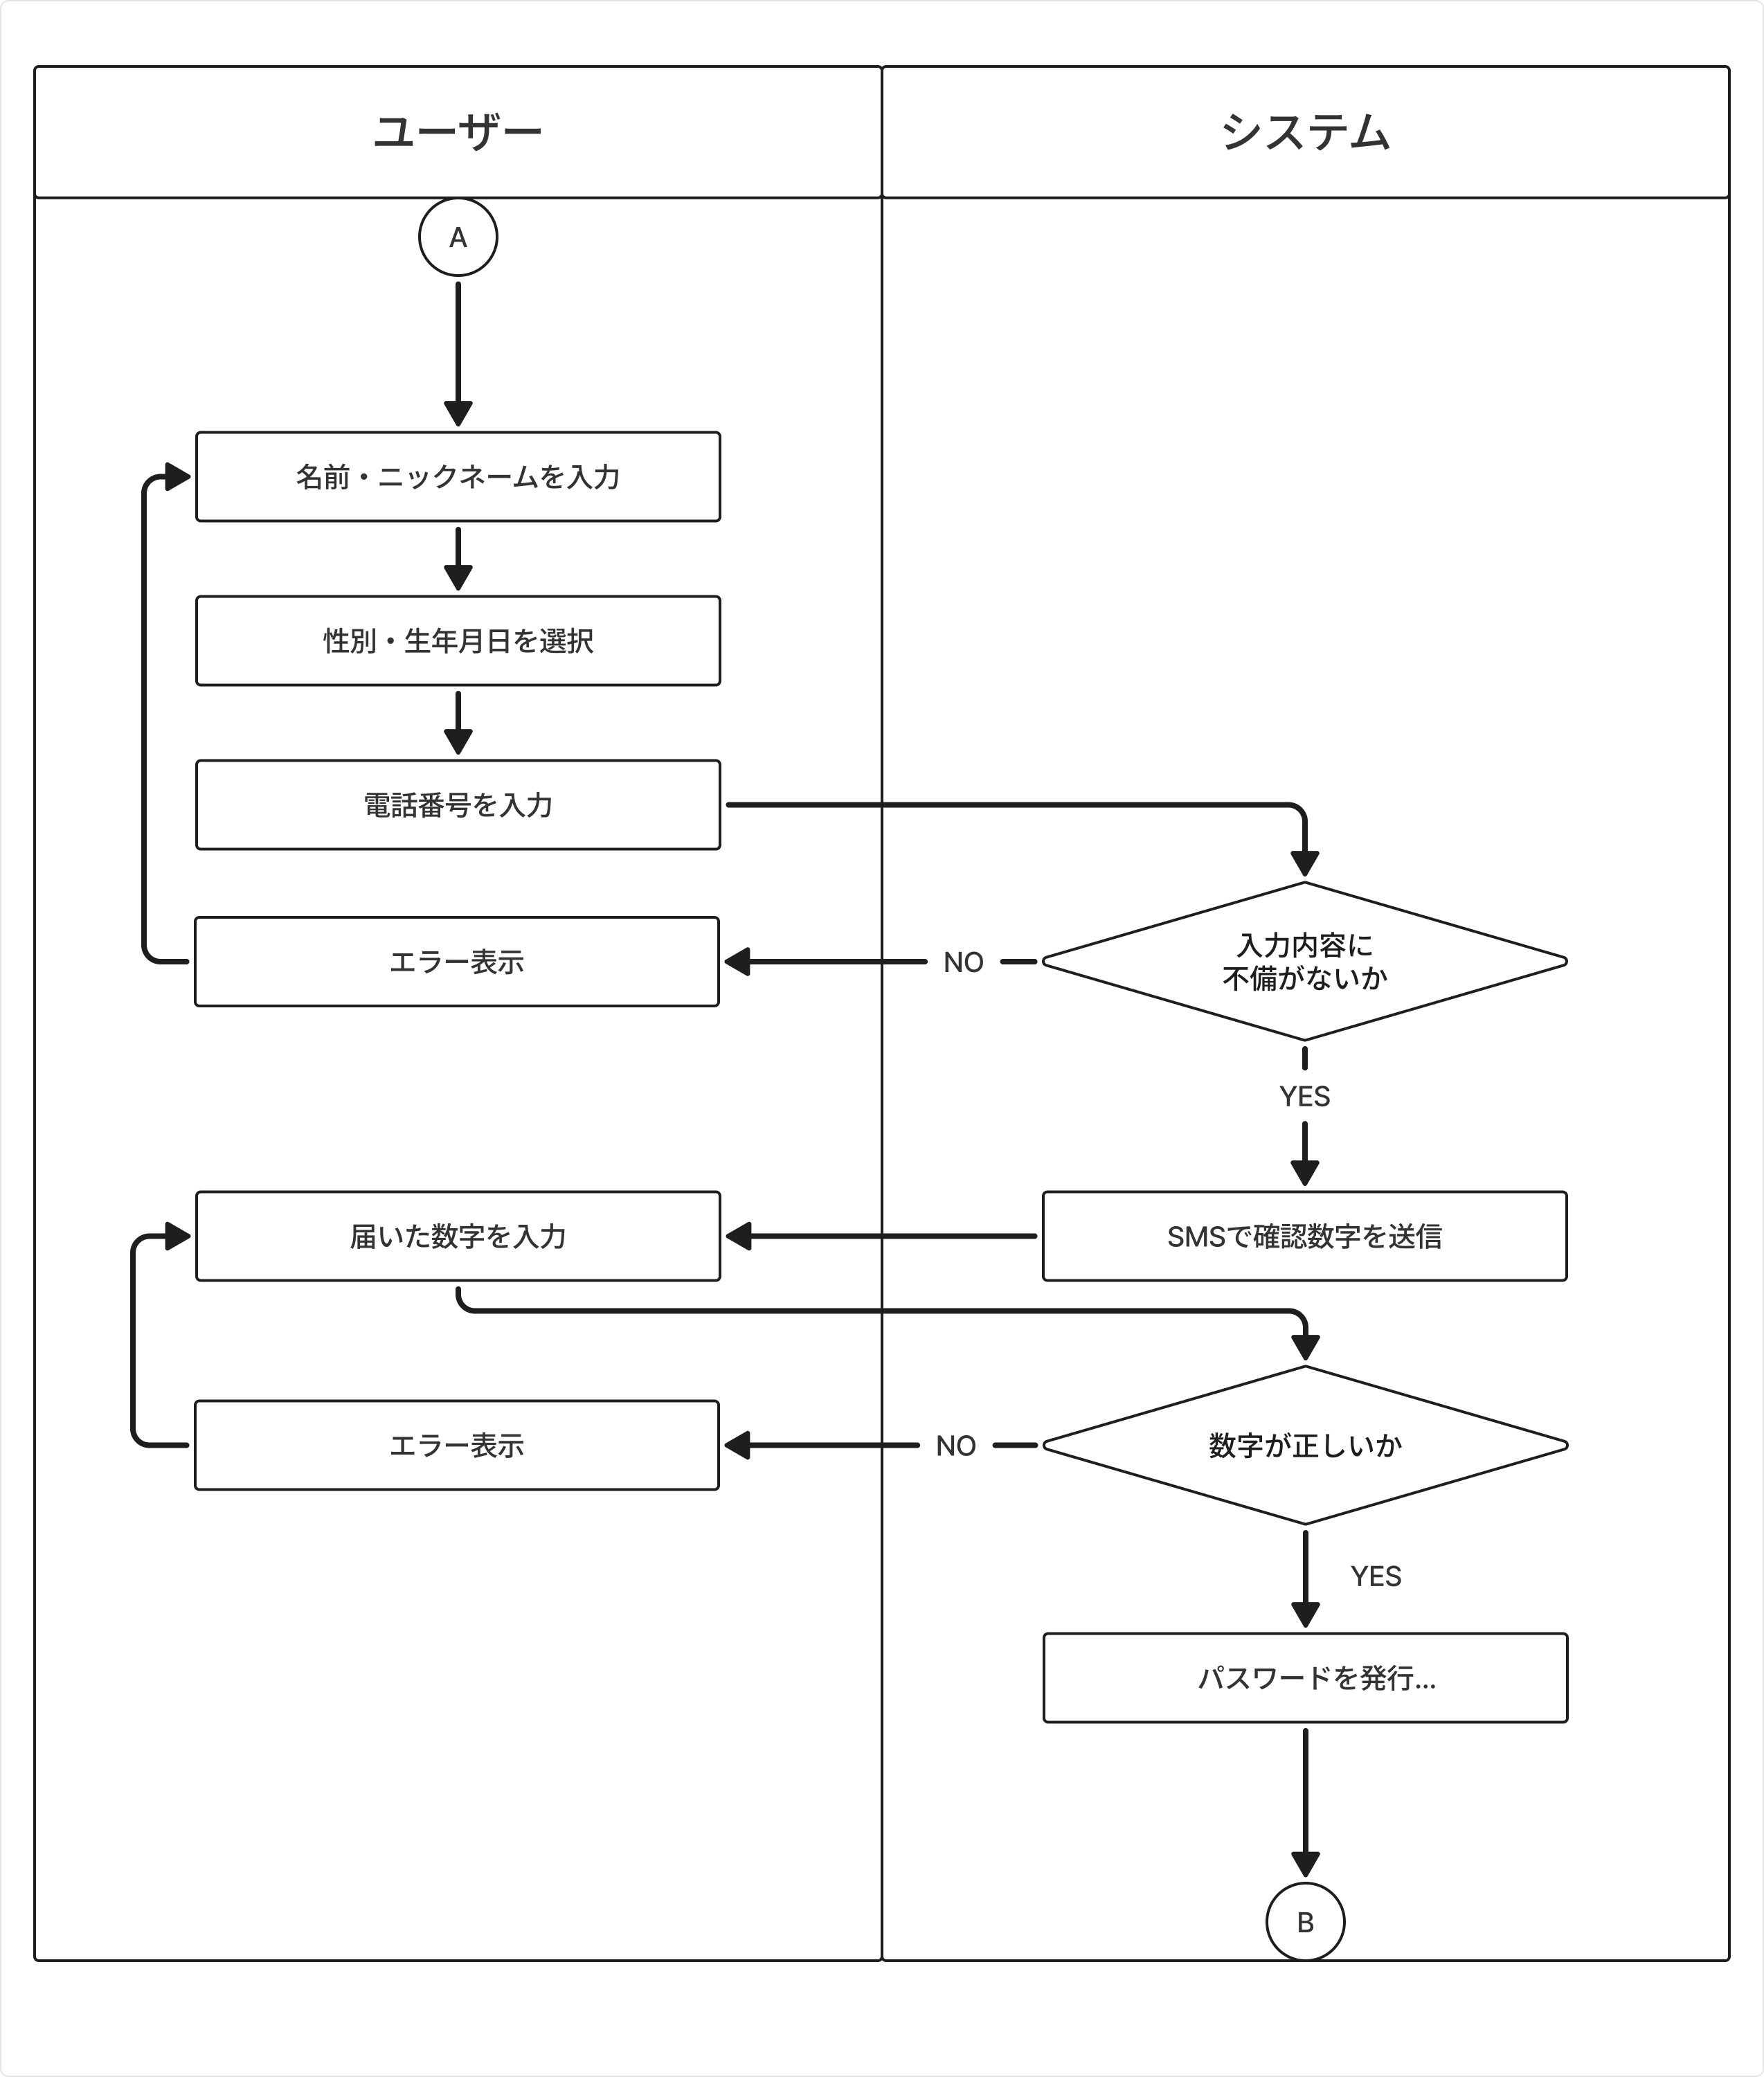
\includegraphics[width=\linewidth]{chapters/images/register2.png}
    \caption{新規会員登録機能のアクティビティ図2（登録情報の入力・SMS確認）}
    \label{fig:register2}
  \end{minipage}
\end{figure}

\begin{figure}[H]
  \centering
  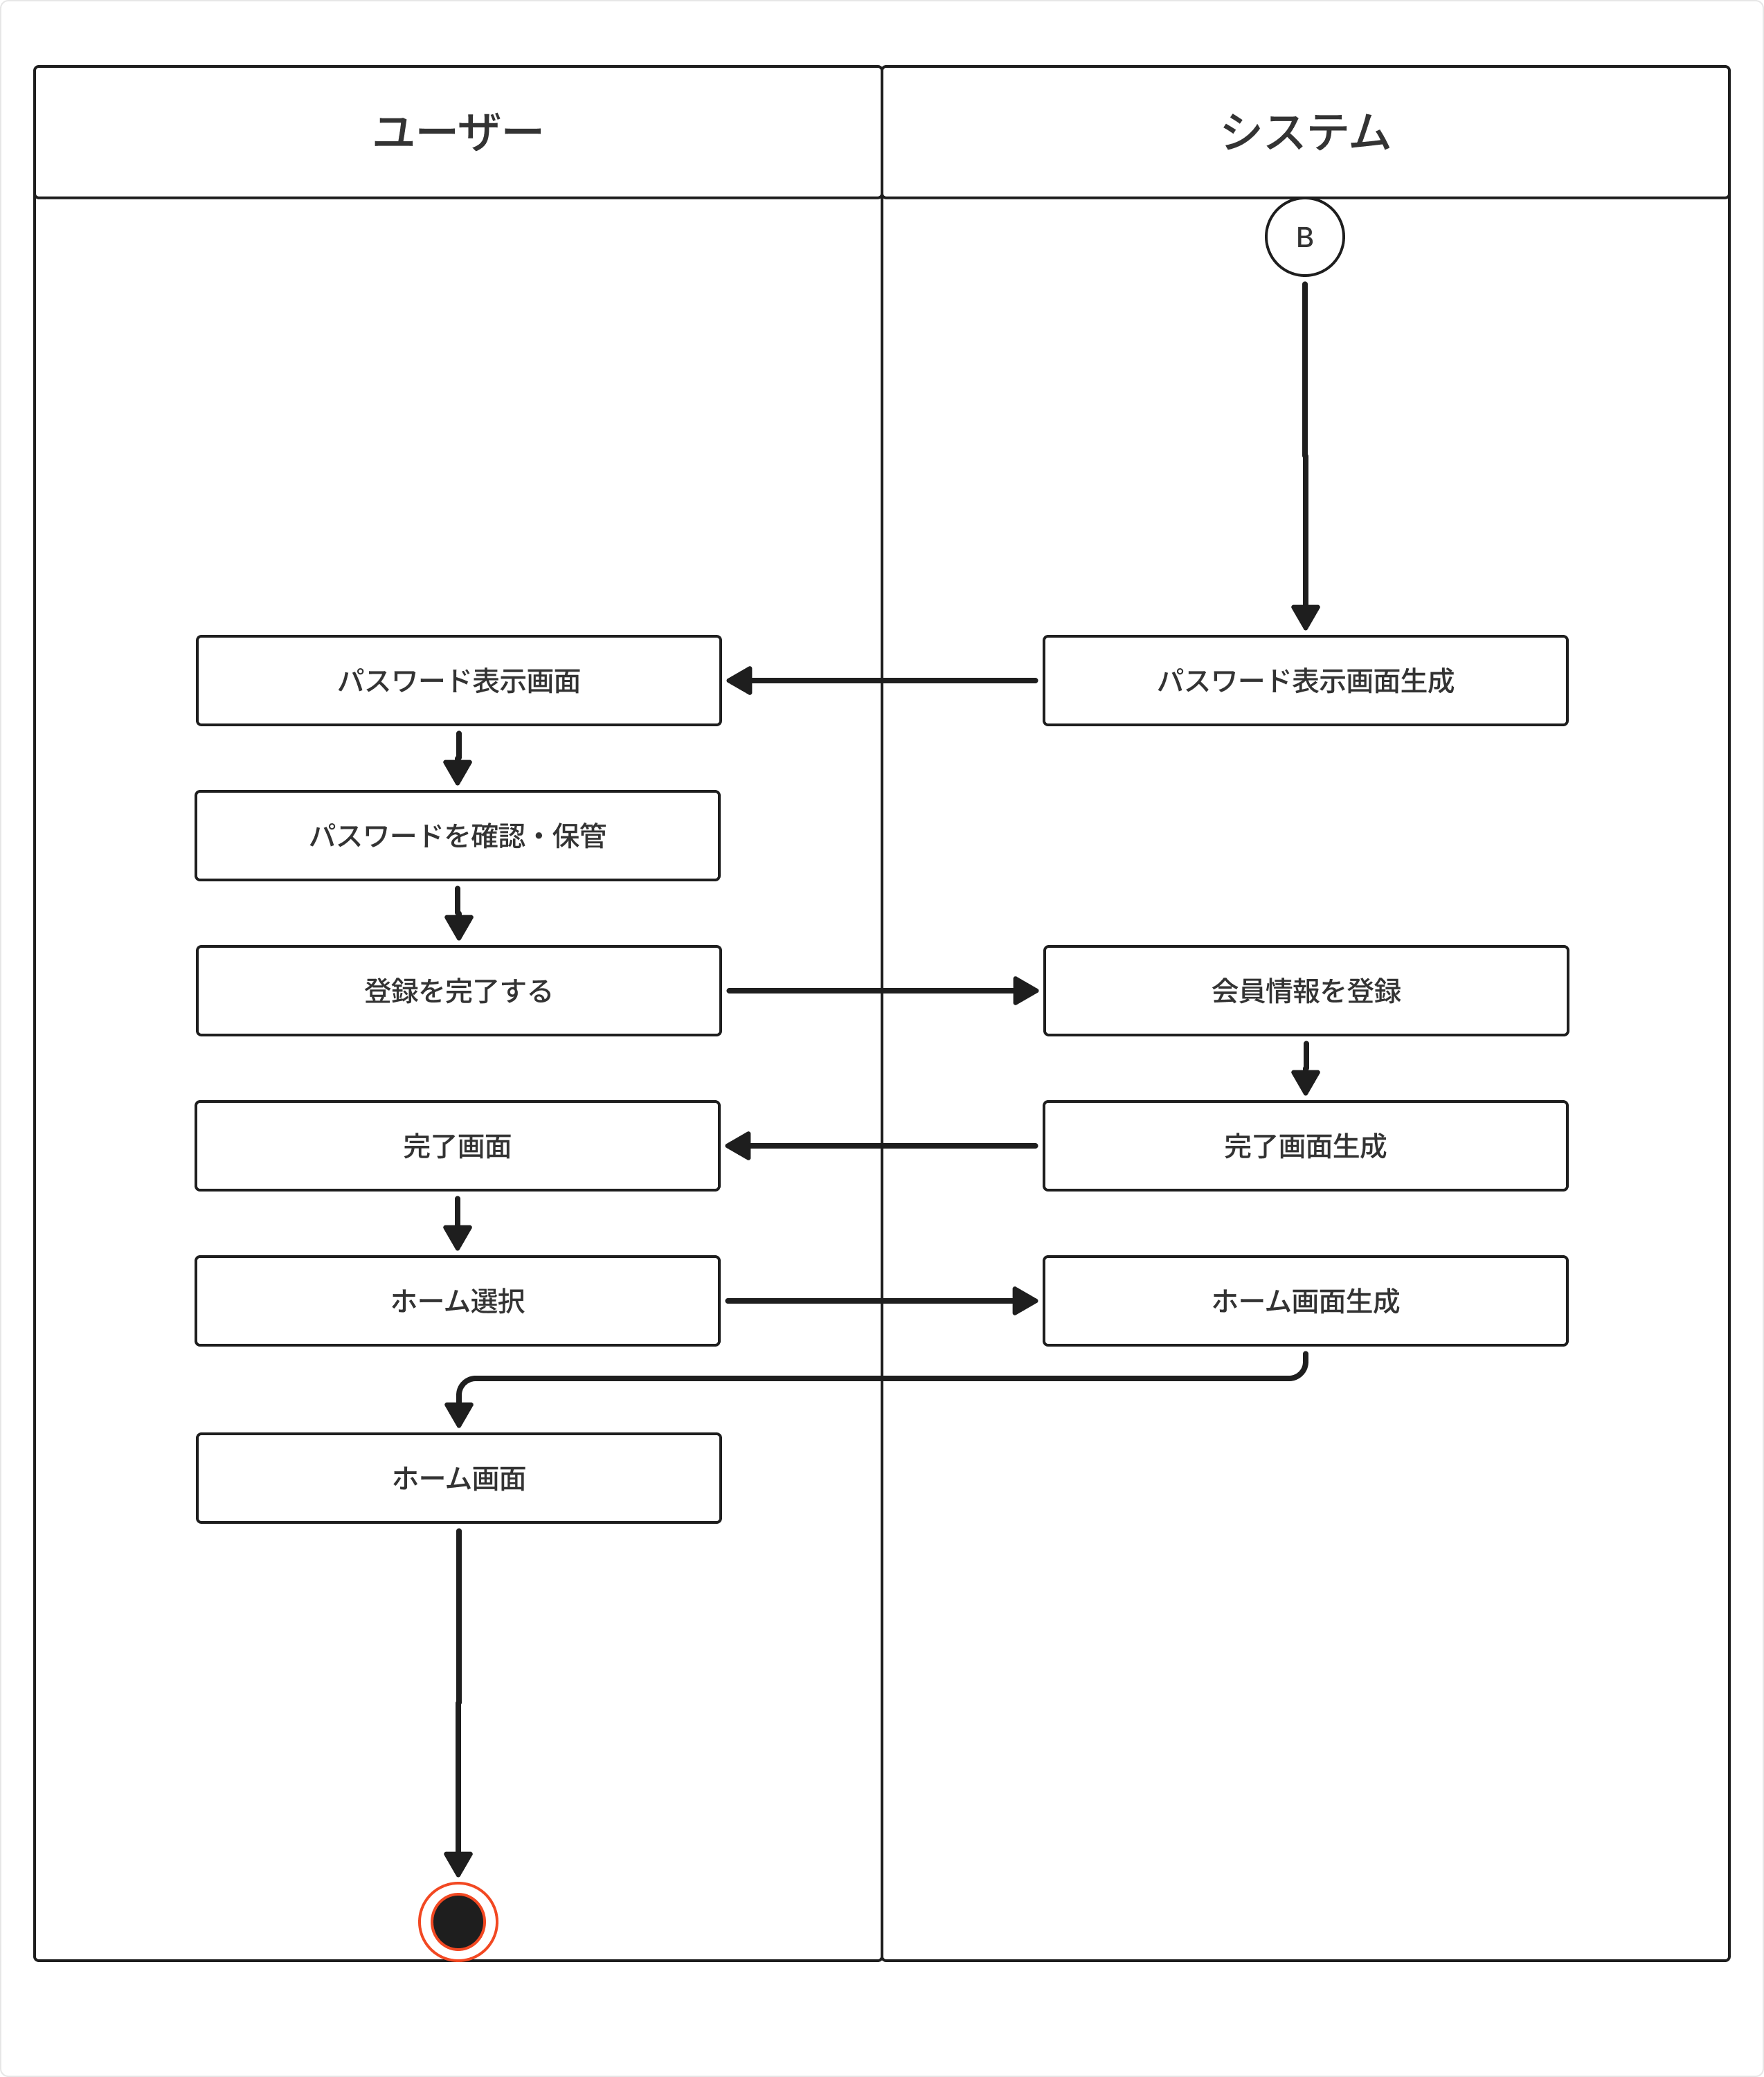
\includegraphics[width=0.48\linewidth]{chapters/images/register3.png}
  \caption{新規会員登録機能のアクティビティ図3（パスワード確認・登録完了）}
  \label{fig:register3}
\end{figure}

%......................................................................
\subsubsection{ログイン機能}\label{subsubsec:login}
%......................................................................
会員登録済みの利用者が, 携帯電話番号を使ってアプリにログインする機能である.
初期画面で「ログイン」を選択し, 携帯電話番号と, パスワードまたは生年月日を入力する.
そのうえで, SMSで届く6桁の数字を入力して確認し, 「ログインする」を選択する.
パスワードを忘れた場合は, パスワードの代わりに生年月日で確認できる.

図\ref{fig:login}にログイン機能の流れを示す.

%......................................................................
\subsubsection{ログアウト機能}\label{subsubsec:logout}
%......................................................................
ログイン中の利用者が, アプリからログアウトする機能である.
ログアウトすると, ゲストとしての利用に切り替わる.

図\ref{fig:logout}にログアウト機能の流れを示す.

\begin{figure}[H]
  \centering
  \begin{minipage}[t]{0.48\linewidth}
    \centering
    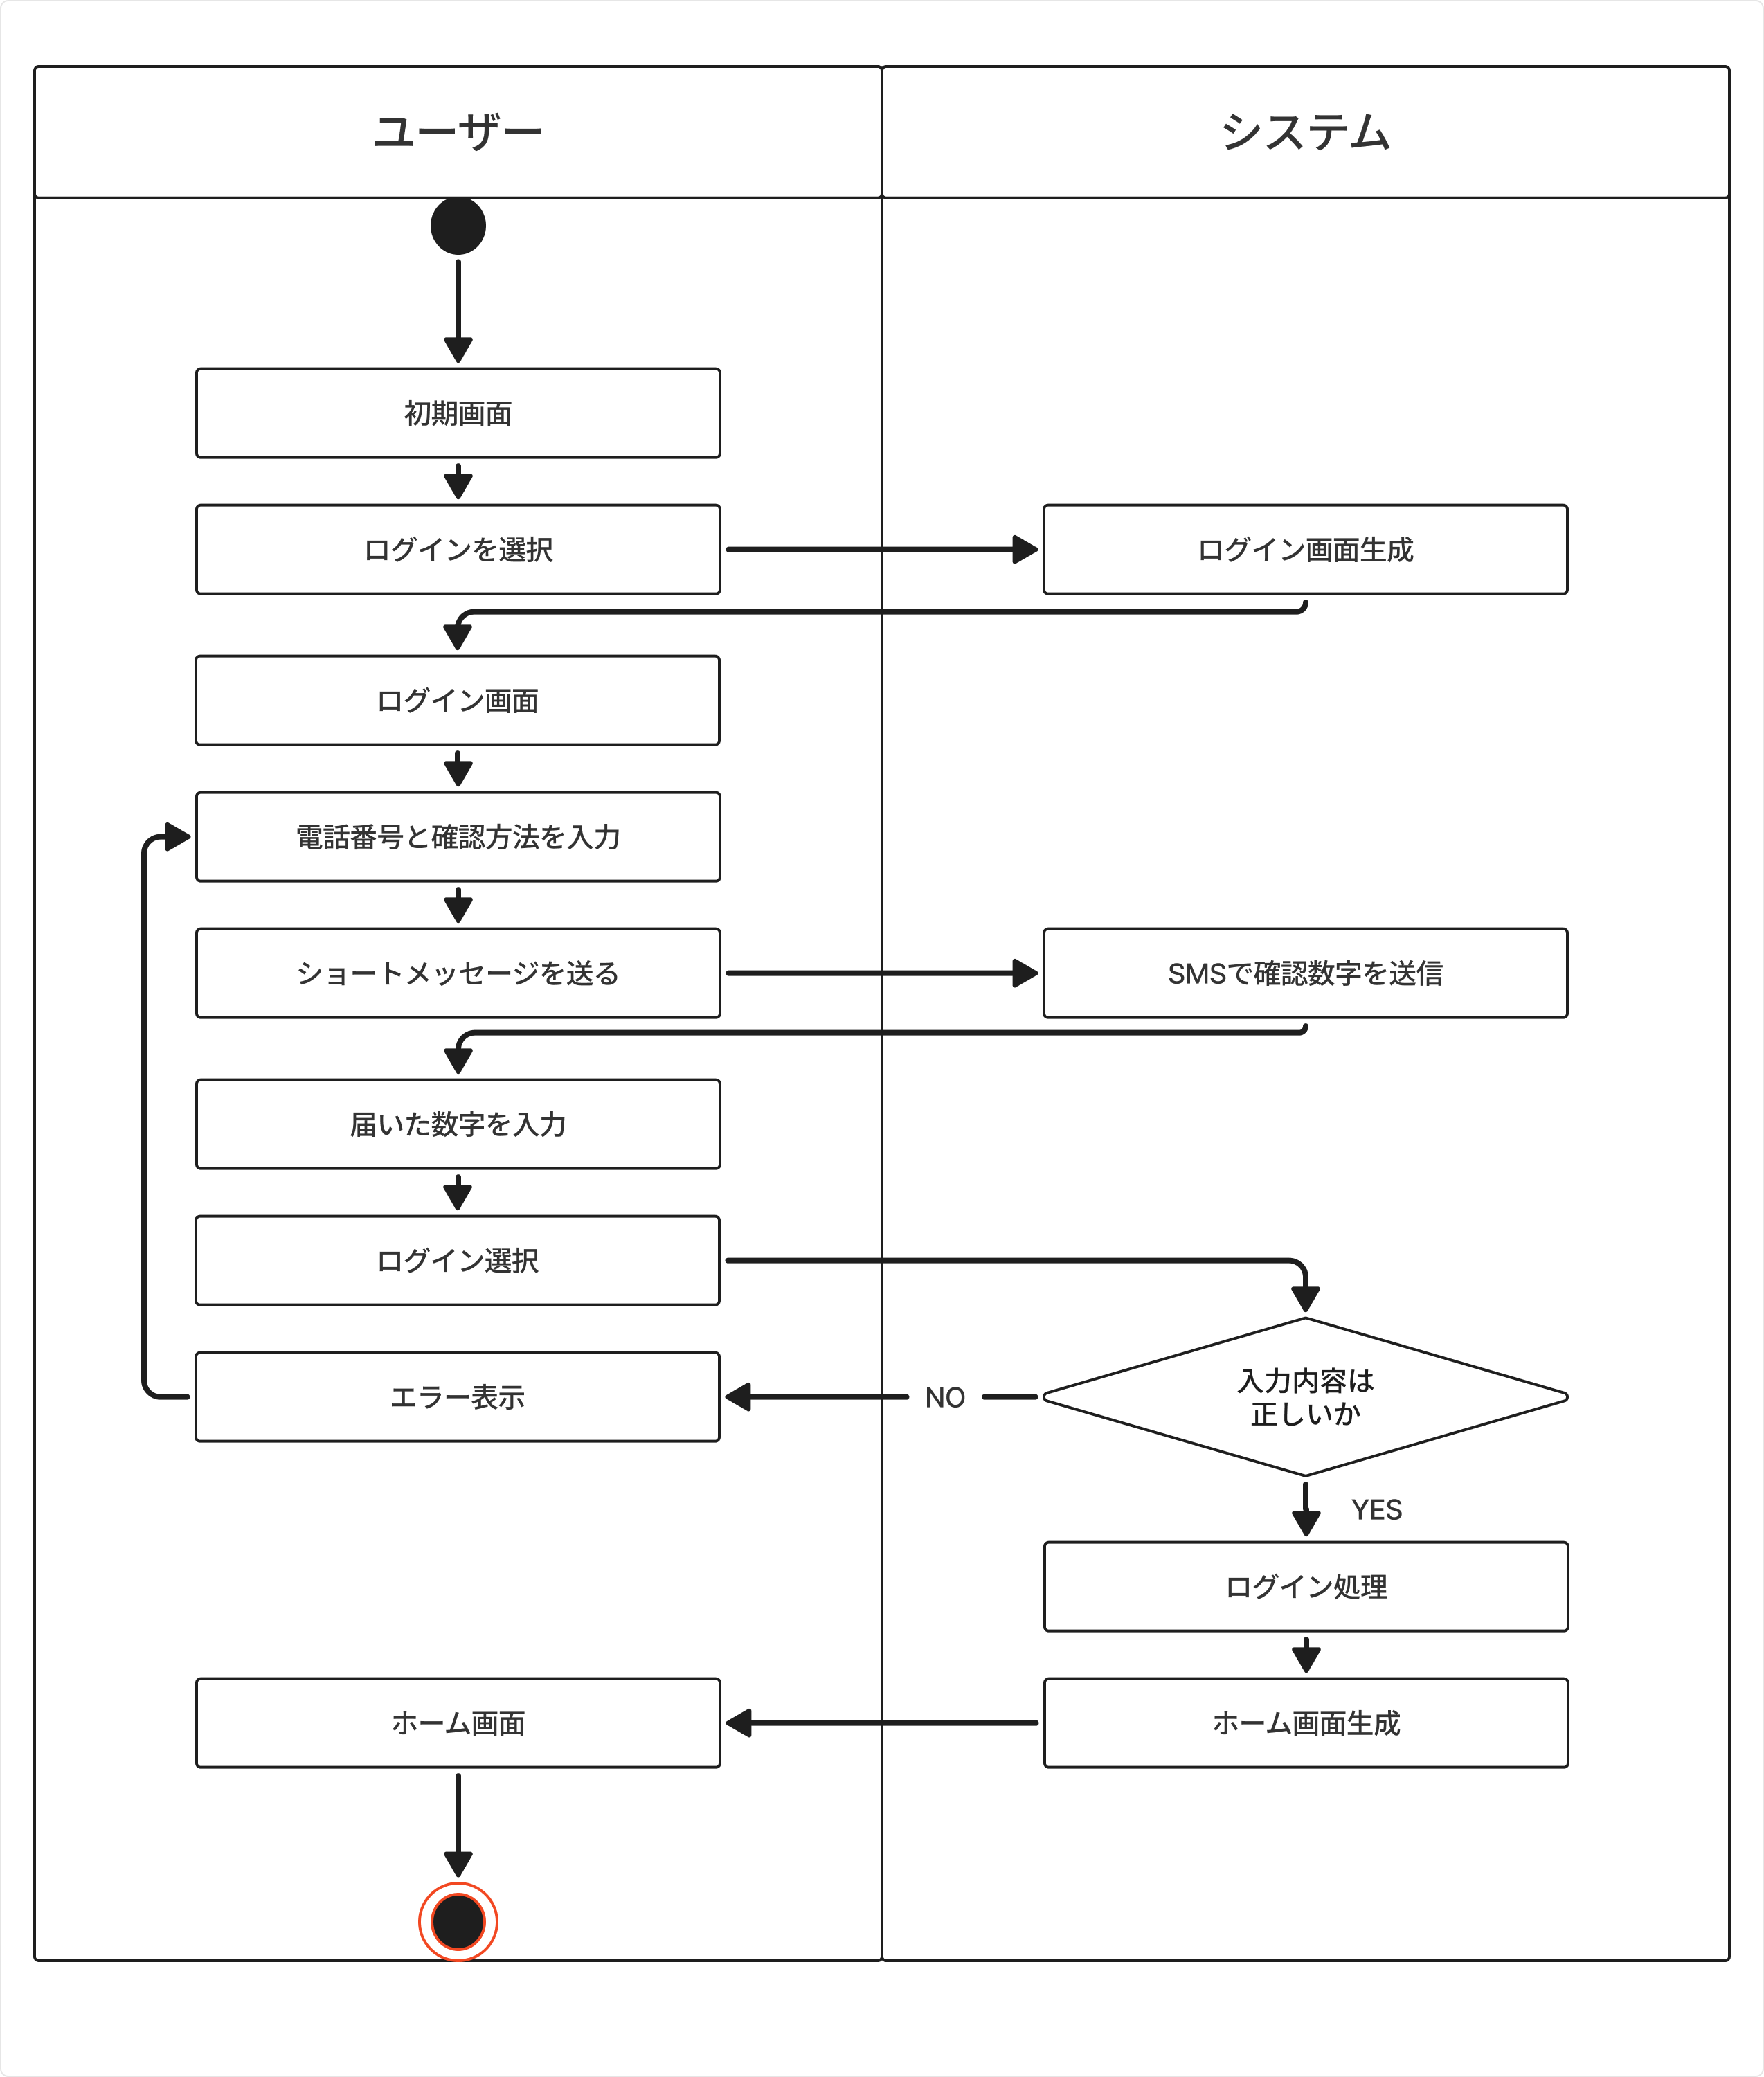
\includegraphics[width=\linewidth]{chapters/images/login.png}
    \caption{ログイン機能のアクティビティ図}
    \label{fig:login}
  \end{minipage}
  \hfill
  \begin{minipage}[t]{0.48\linewidth}
    \centering
    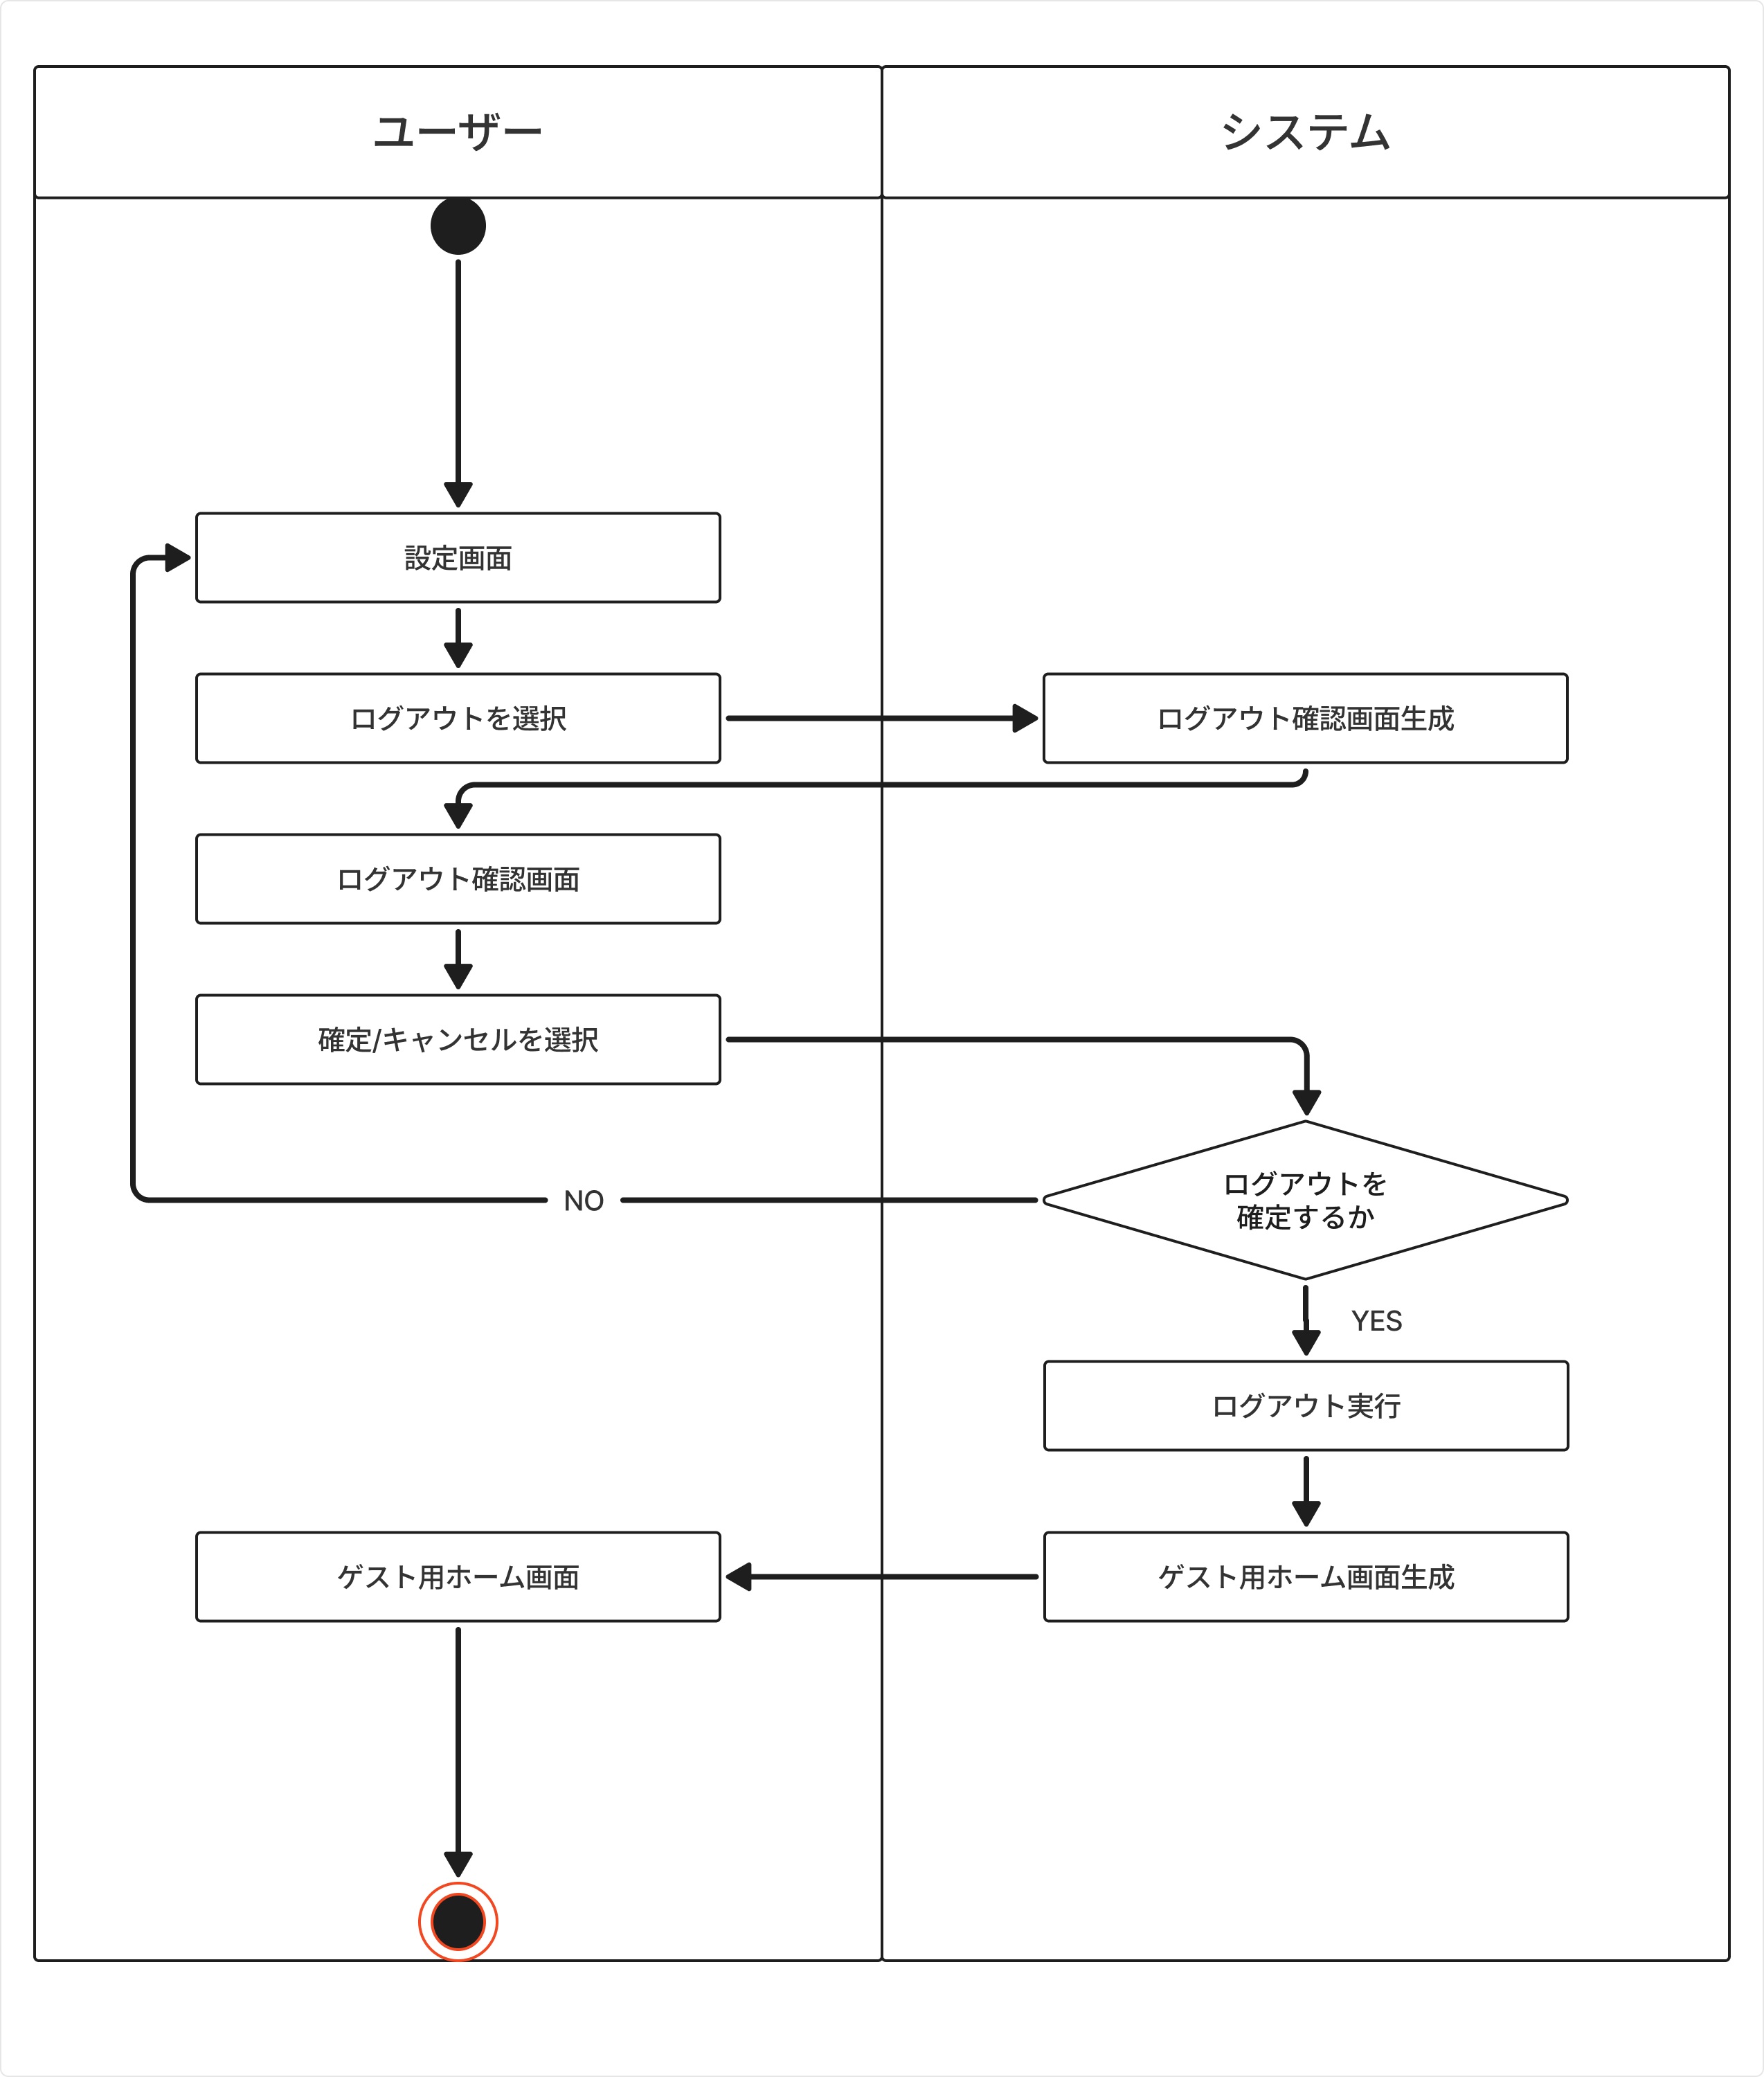
\includegraphics[width=\linewidth]{chapters/images/logout.png}
    \caption{ログアウト機能のアクティビティ図}
    \label{fig:logout}
  \end{minipage}
\end{figure}

%......................................................................
\subsubsection{会員情報変更機能}\label{subsubsec:member-edit}
%......................................................................
利用者が, 登録済みの会員情報の確認と変更を, 利用者ごとのマイページから行う機能である.
マイページには自分のプロフィールが表示され, 変更できる項目はニックネームとパスワードとする.

図\ref{fig:member-edit}に会員情報変更機能の流れを示す.

\begin{figure}[H]
  \centering
  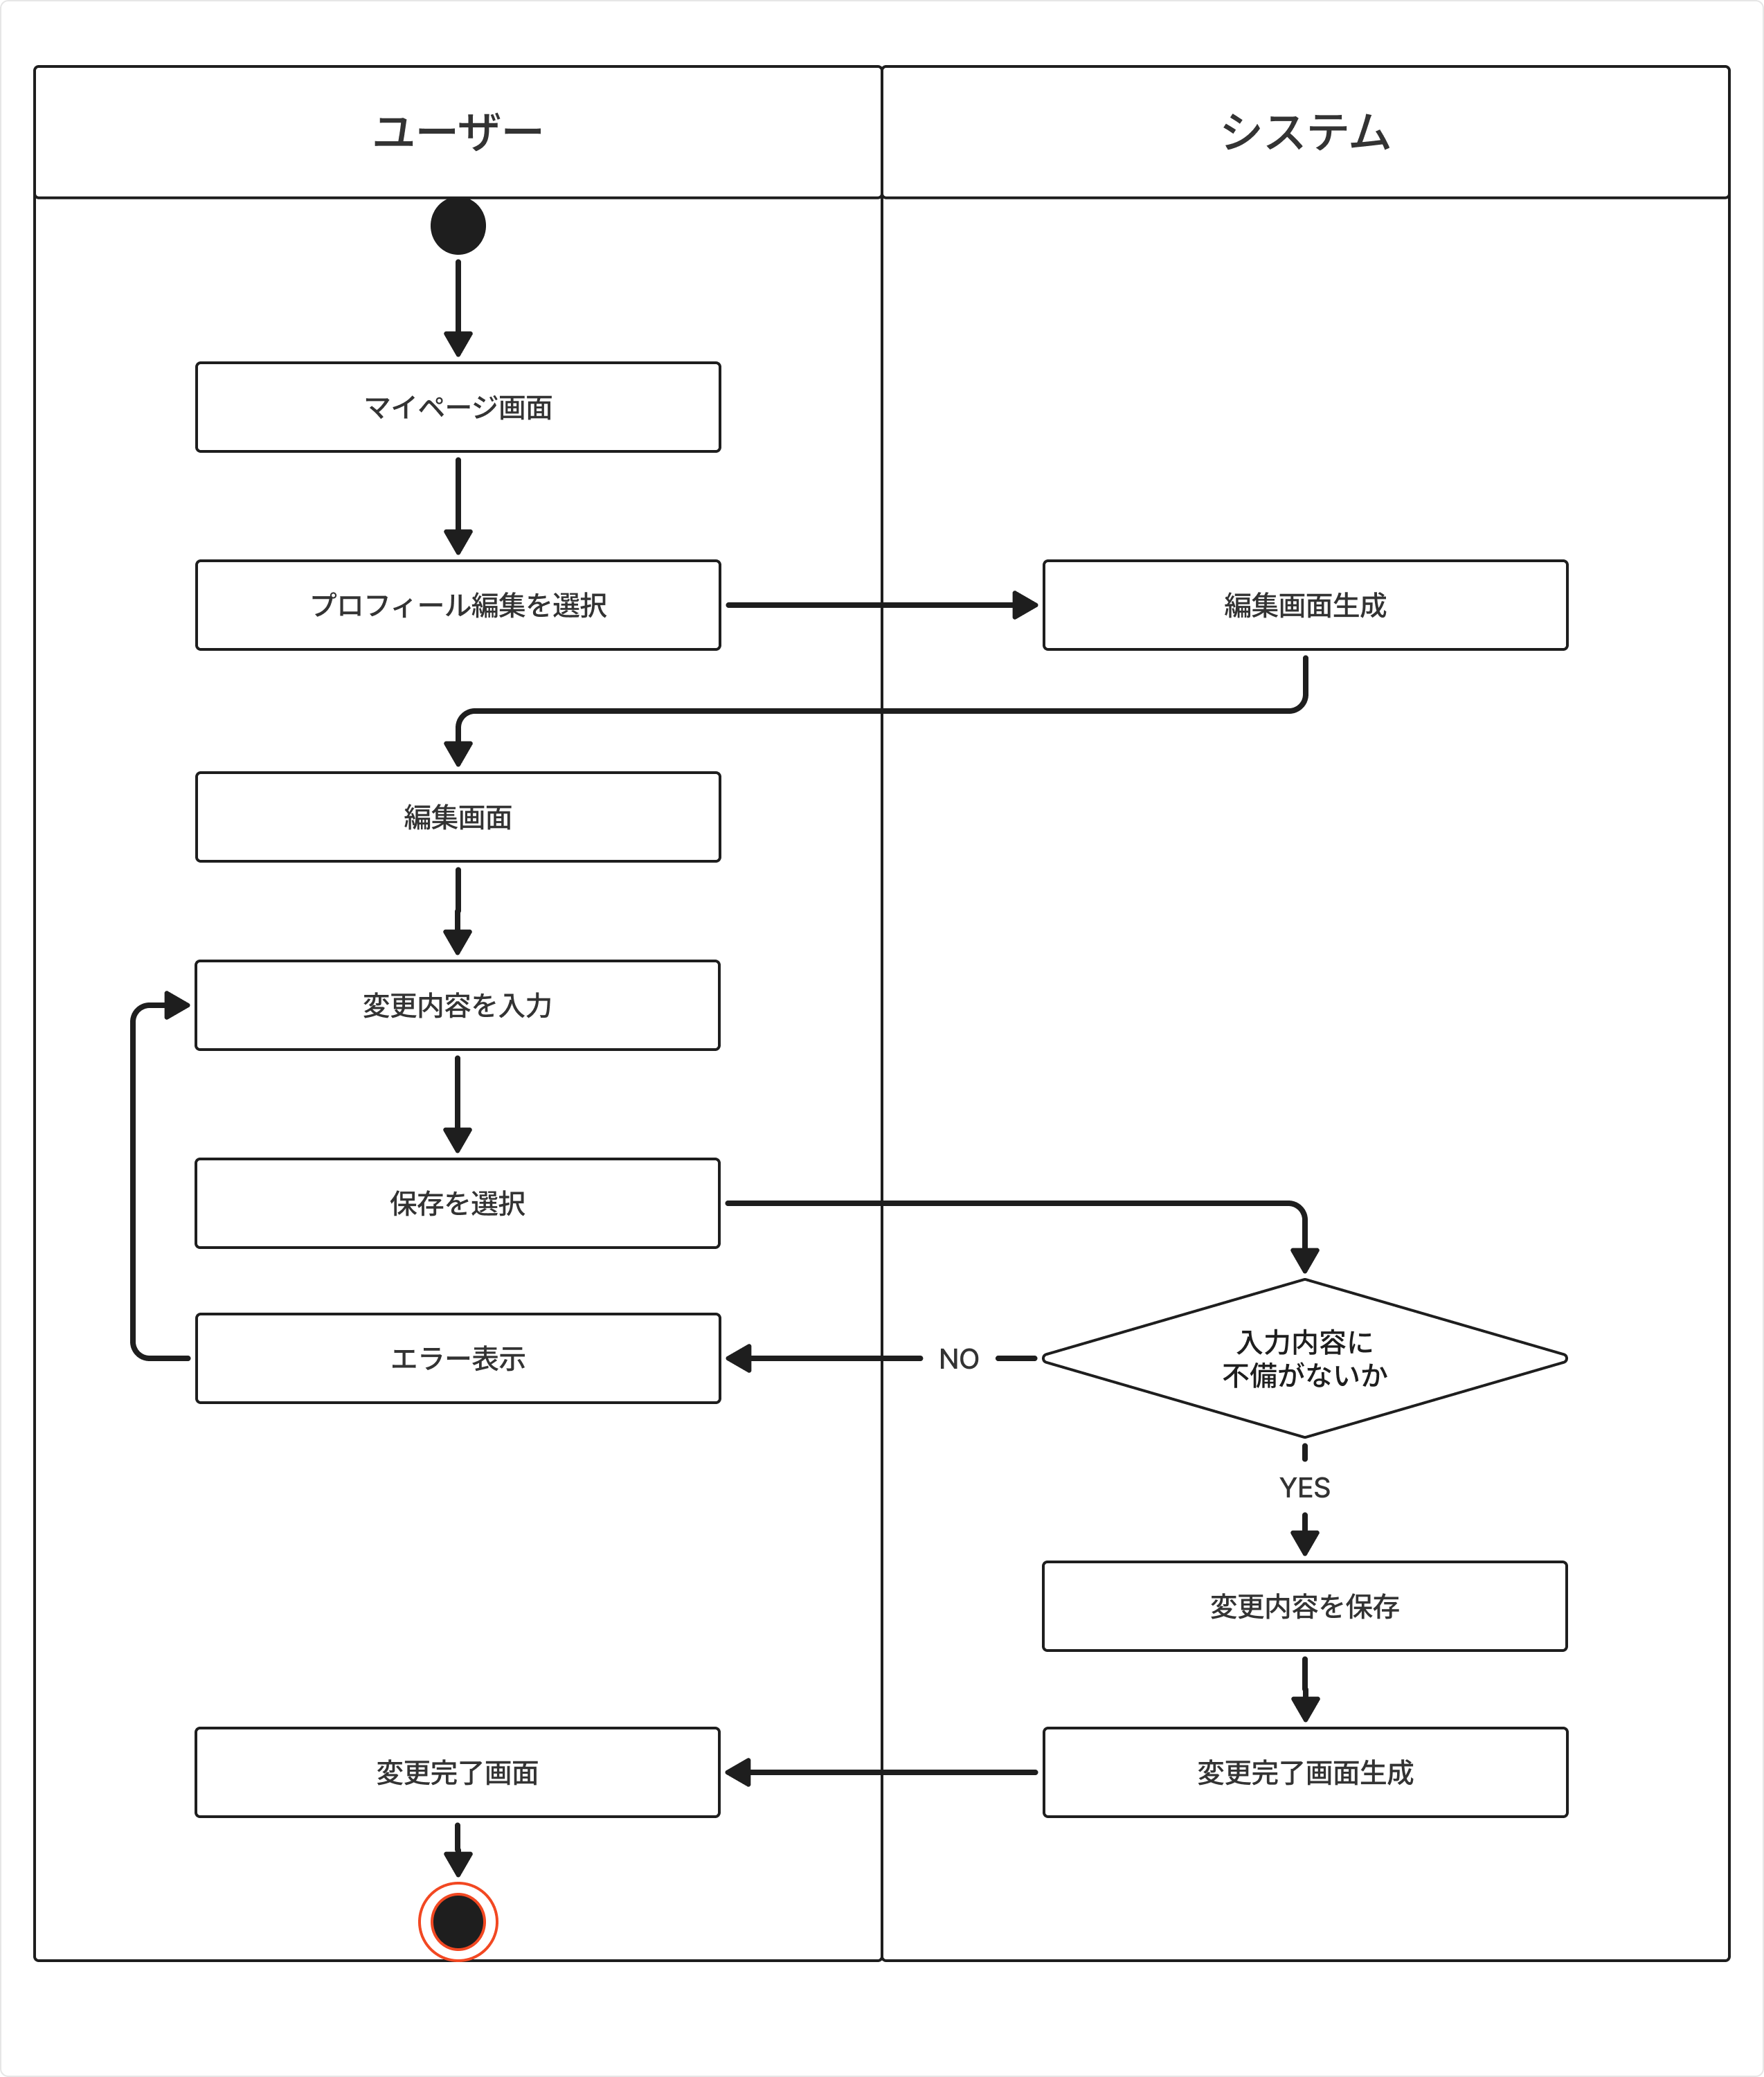
\includegraphics[width=0.48\linewidth]{chapters/images/member_edit.png}
  \caption{会員情報変更機能のアクティビティ図}
  \label{fig:member-edit}
\end{figure}

%......................................................................
\subsubsection{投稿評価機能}\label{subsubsec:reaction}
%......................................................................
閲覧中の投稿が役に立ったときに, 投稿の下部にある$\heartsuit$ボタンを押して, 投稿者にリアクションを送る機能である.
リアクションの種類は$\heartsuit$のみとし, 送られた$\heartsuit$の数に応じて投稿者にポイントが加算される.

図\ref{fig:reaction}に投稿評価機能の流れを示す.

%......................................................................
\subsubsection{投稿保存機能}\label{subsubsec:post-save}
%......................................................................
閲覧中の投稿を, 投稿の下部にある保存ボタンから保存する機能である.
保存した投稿は, マイページの「保存した投稿」一覧から, いつでも見返すことができる.

図\ref{fig:post-save}に投稿保存機能の流れを示す.

\begin{figure}[H]
  \centering
  \begin{minipage}[t]{0.48\linewidth}
    \centering
    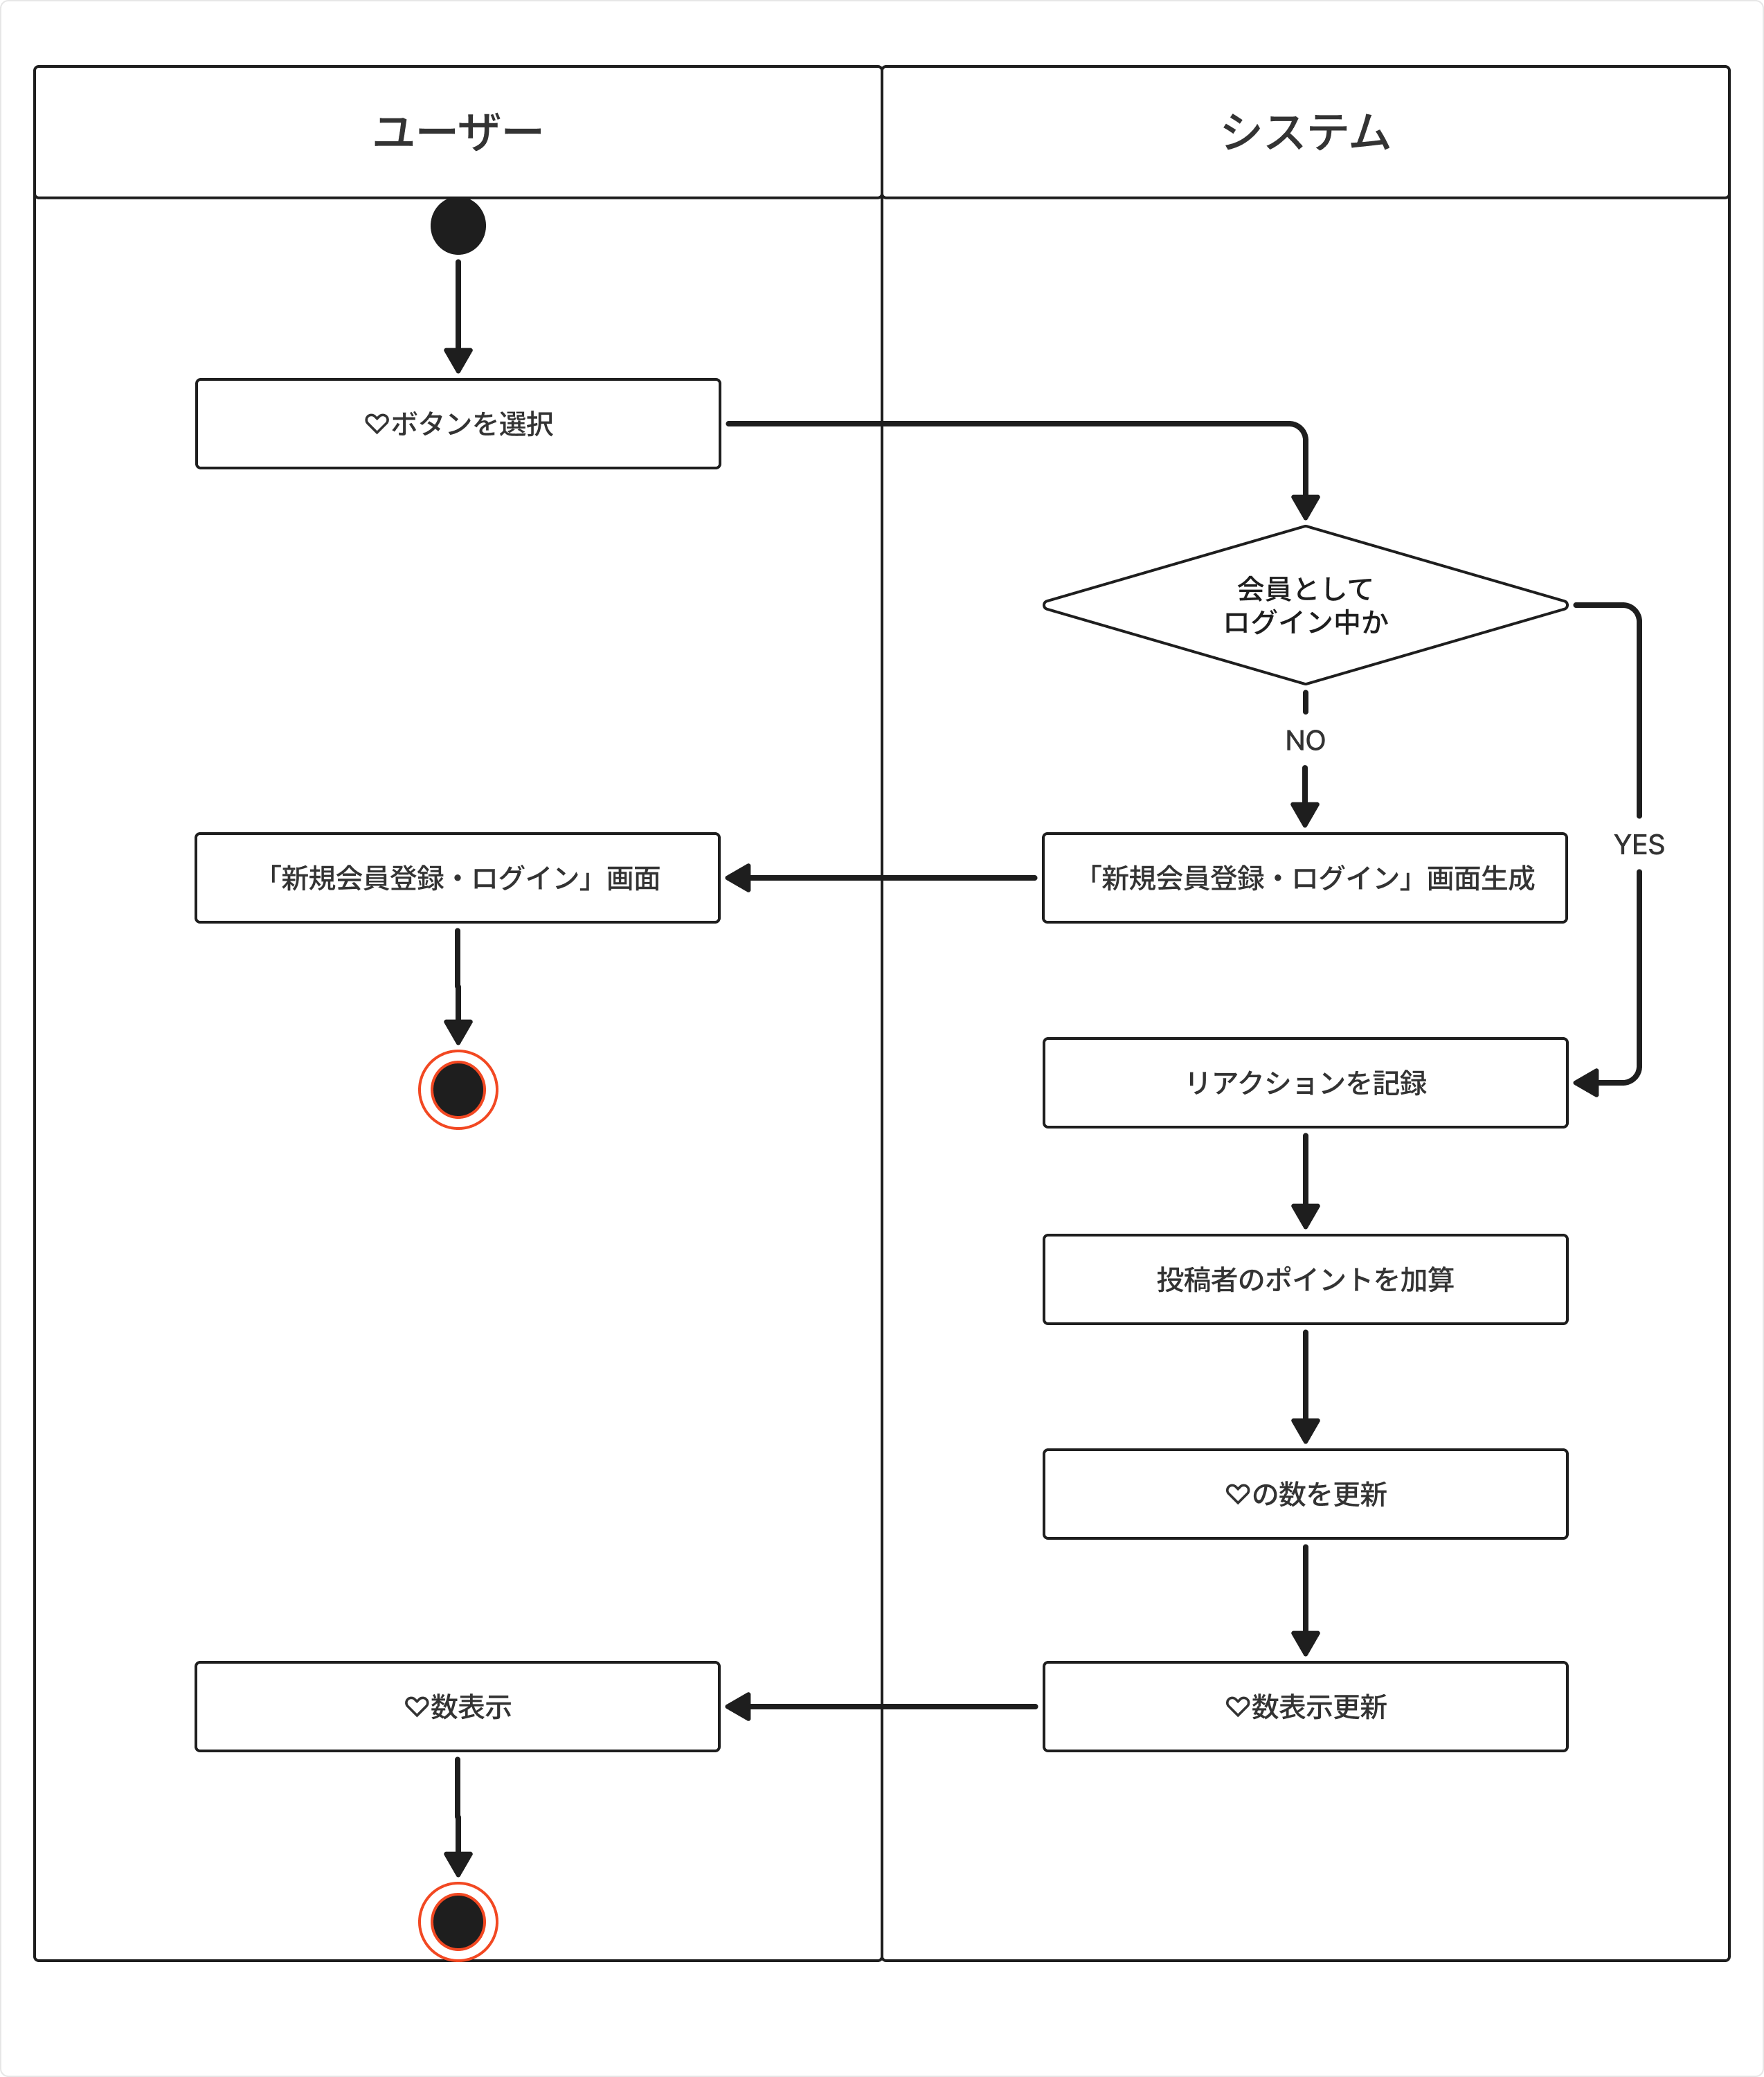
\includegraphics[width=\linewidth]{chapters/images/reaction.png}
    \caption{投稿評価機能のアクティビティ図}
    \label{fig:reaction}
  \end{minipage}
  \hfill
  \begin{minipage}[t]{0.48\linewidth}
    \centering
    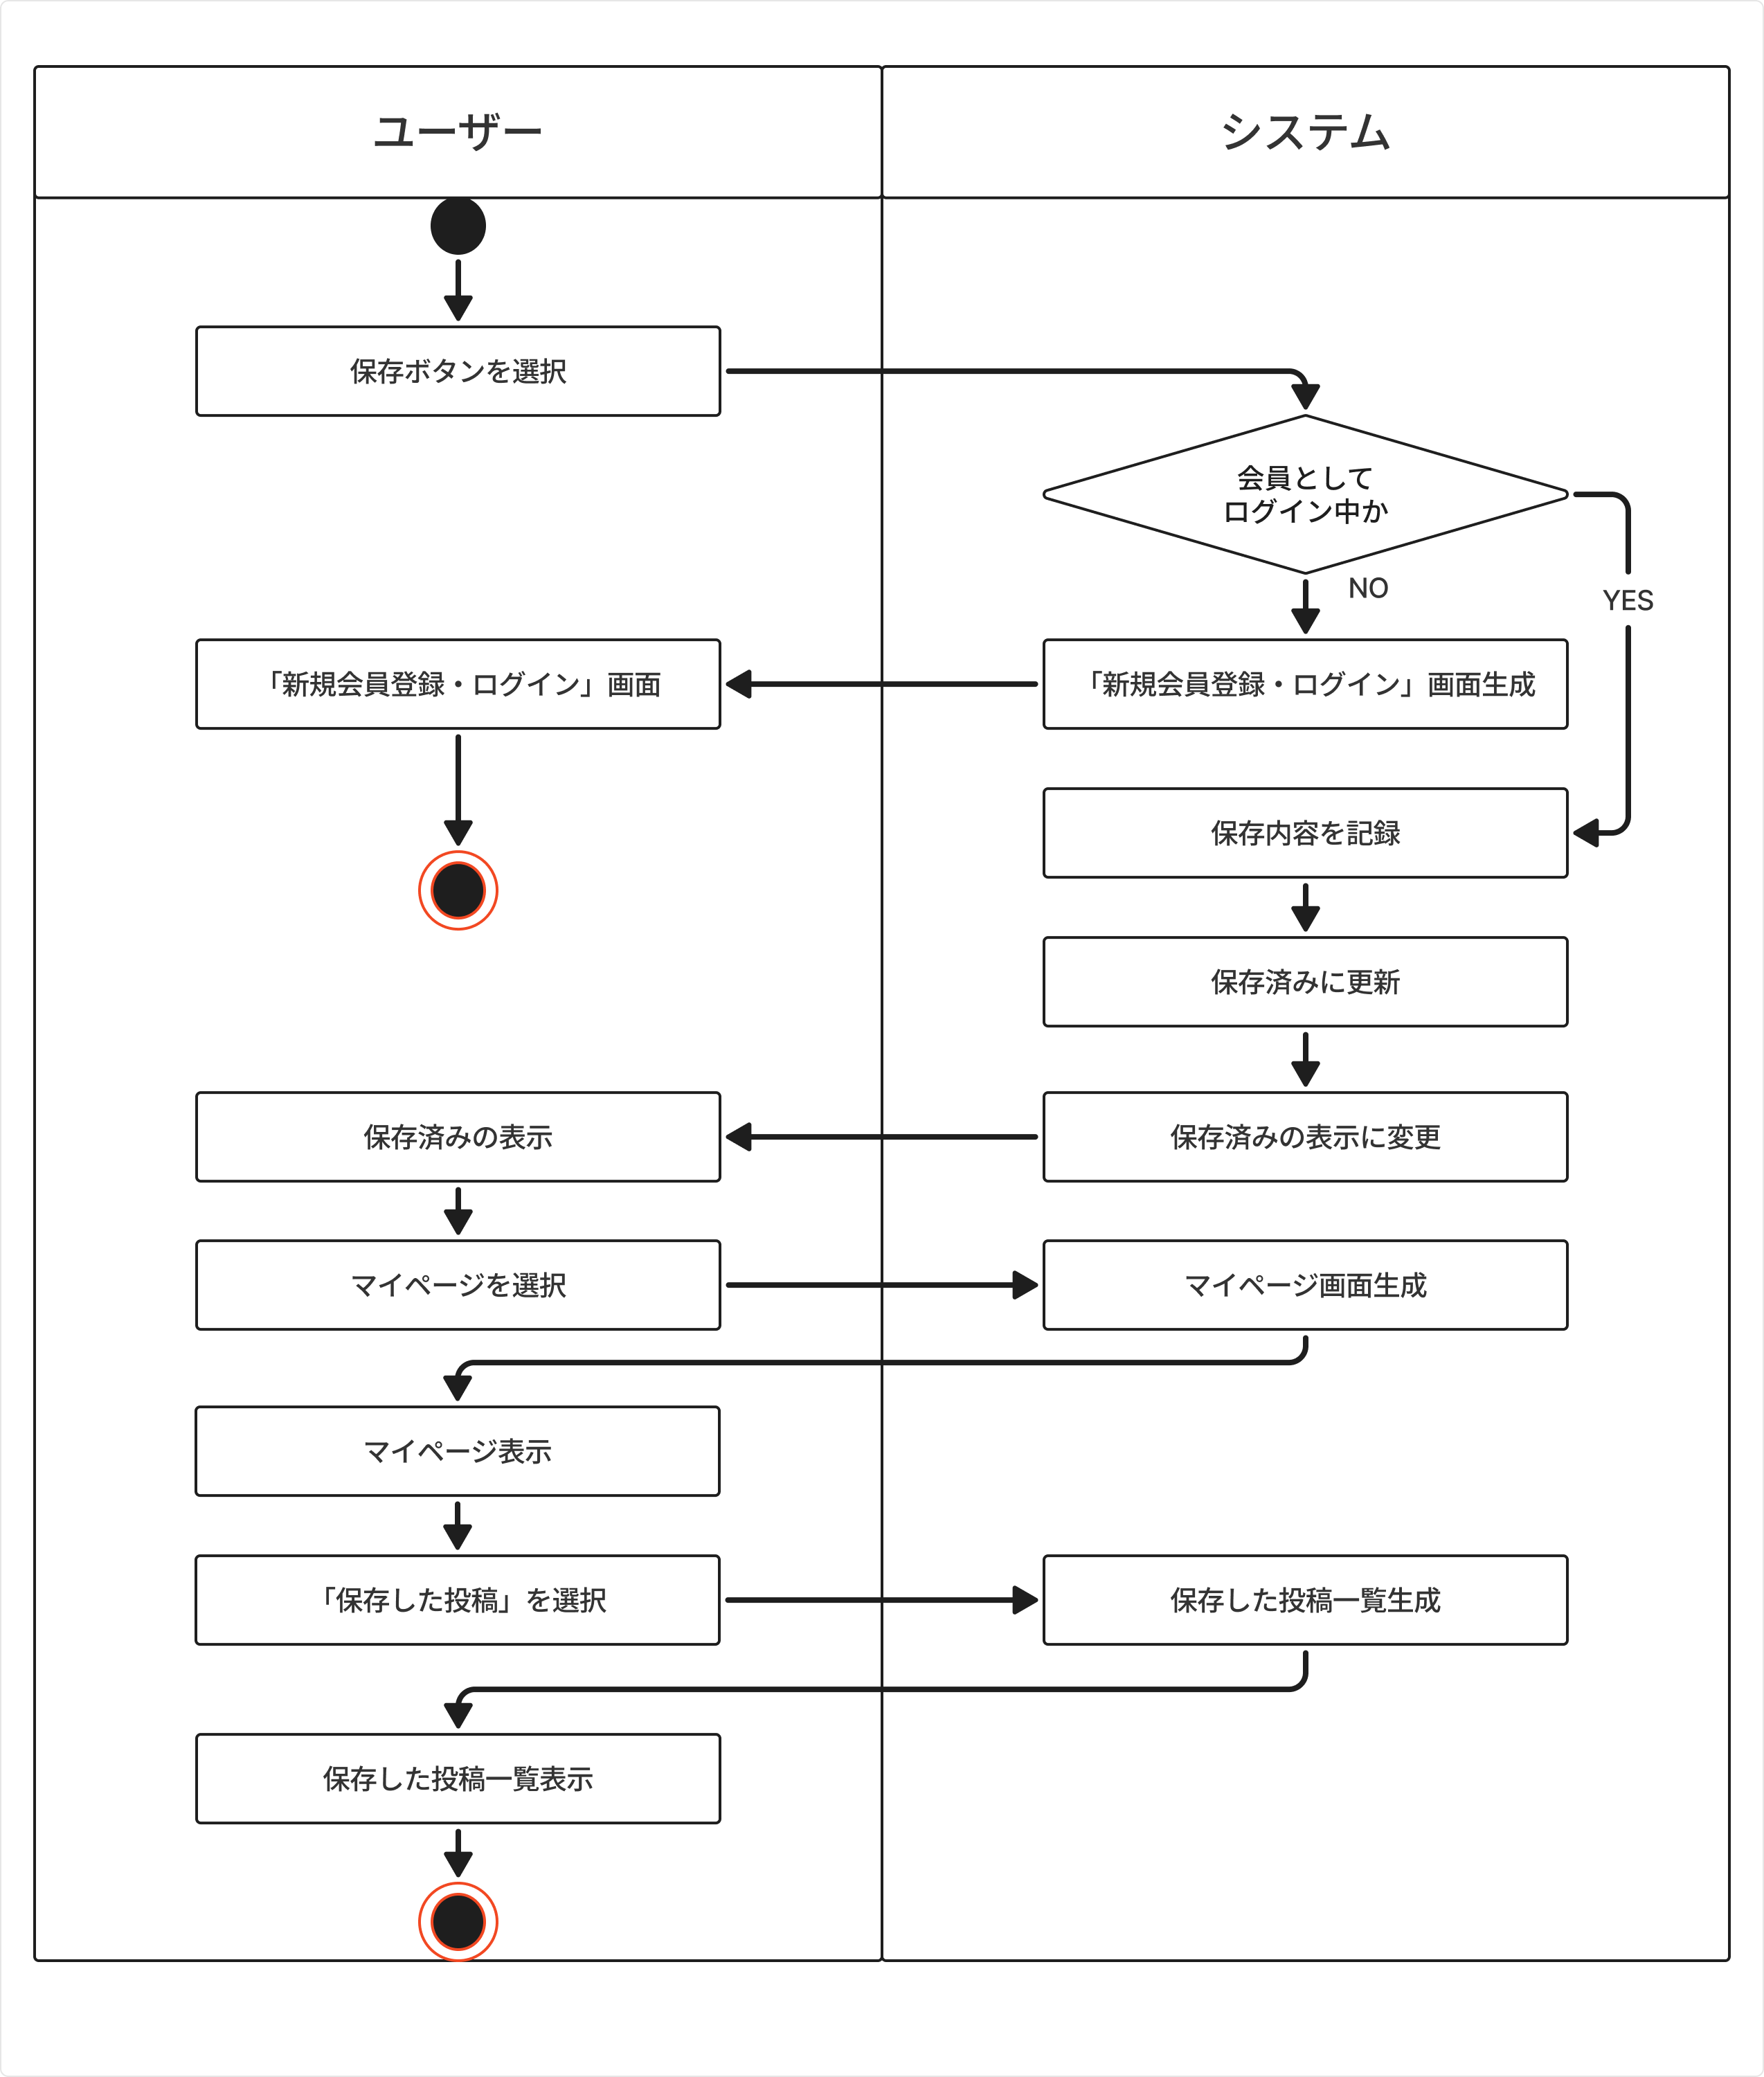
\includegraphics[width=\linewidth]{chapters/images/post_save.png}
    \caption{投稿保存機能のアクティビティ図}
    \label{fig:post-save}
  \end{minipage}
\end{figure}

\subsection{学習者機能}\label{subsec:learner}
%----------------------------------------------------------------------
本項では, 利用目的として「学習者」を選択した会員ユーザが利用する機能について述べる.
各機能の処理の流れは, ユーザとシステムの2つのレーンに分けたアクティビティ図で示す.

%......................................................................
\subsubsection{返信機能}\label{subsubsec:reply}
%......................................................................
閲覧中の投稿に対して, 投稿の下部にあるメッセージボタンから, 追加の質問や疑問点を書き込む機能である.
書き込んだ内容は投稿者に通知され, 投稿者からの回答も学習者に通知されて, 同じ投稿上で確認できる.
書き込みと回答は投稿のコメントとして一覧で表示され, 他の利用者も閲覧できる.

図\ref{fig:reply}に返信機能の流れを示す.
%......................................................................
\subsubsection{質問機能}\label{subsubsec:question}
%......................................................................
学習者が, 回答してほしい投稿者を指定して, 個別に質問を送る機能である.
投稿者のアイコンなどに表示される手紙ボタンから, 質問内容を入力して送信する.
質問は指定した投稿者にのみ届き, 回答も質問した学習者にのみ届く.
この点で, 投稿上で誰でも閲覧できる返信機能（\ref{subsubsec:reply}）とは異なる.

図\ref{fig:act-question}に質問機能の流れを示す.

\begin{figure}[H]
  \centering
  \begin{minipage}[t]{0.48\linewidth}
    \centering
    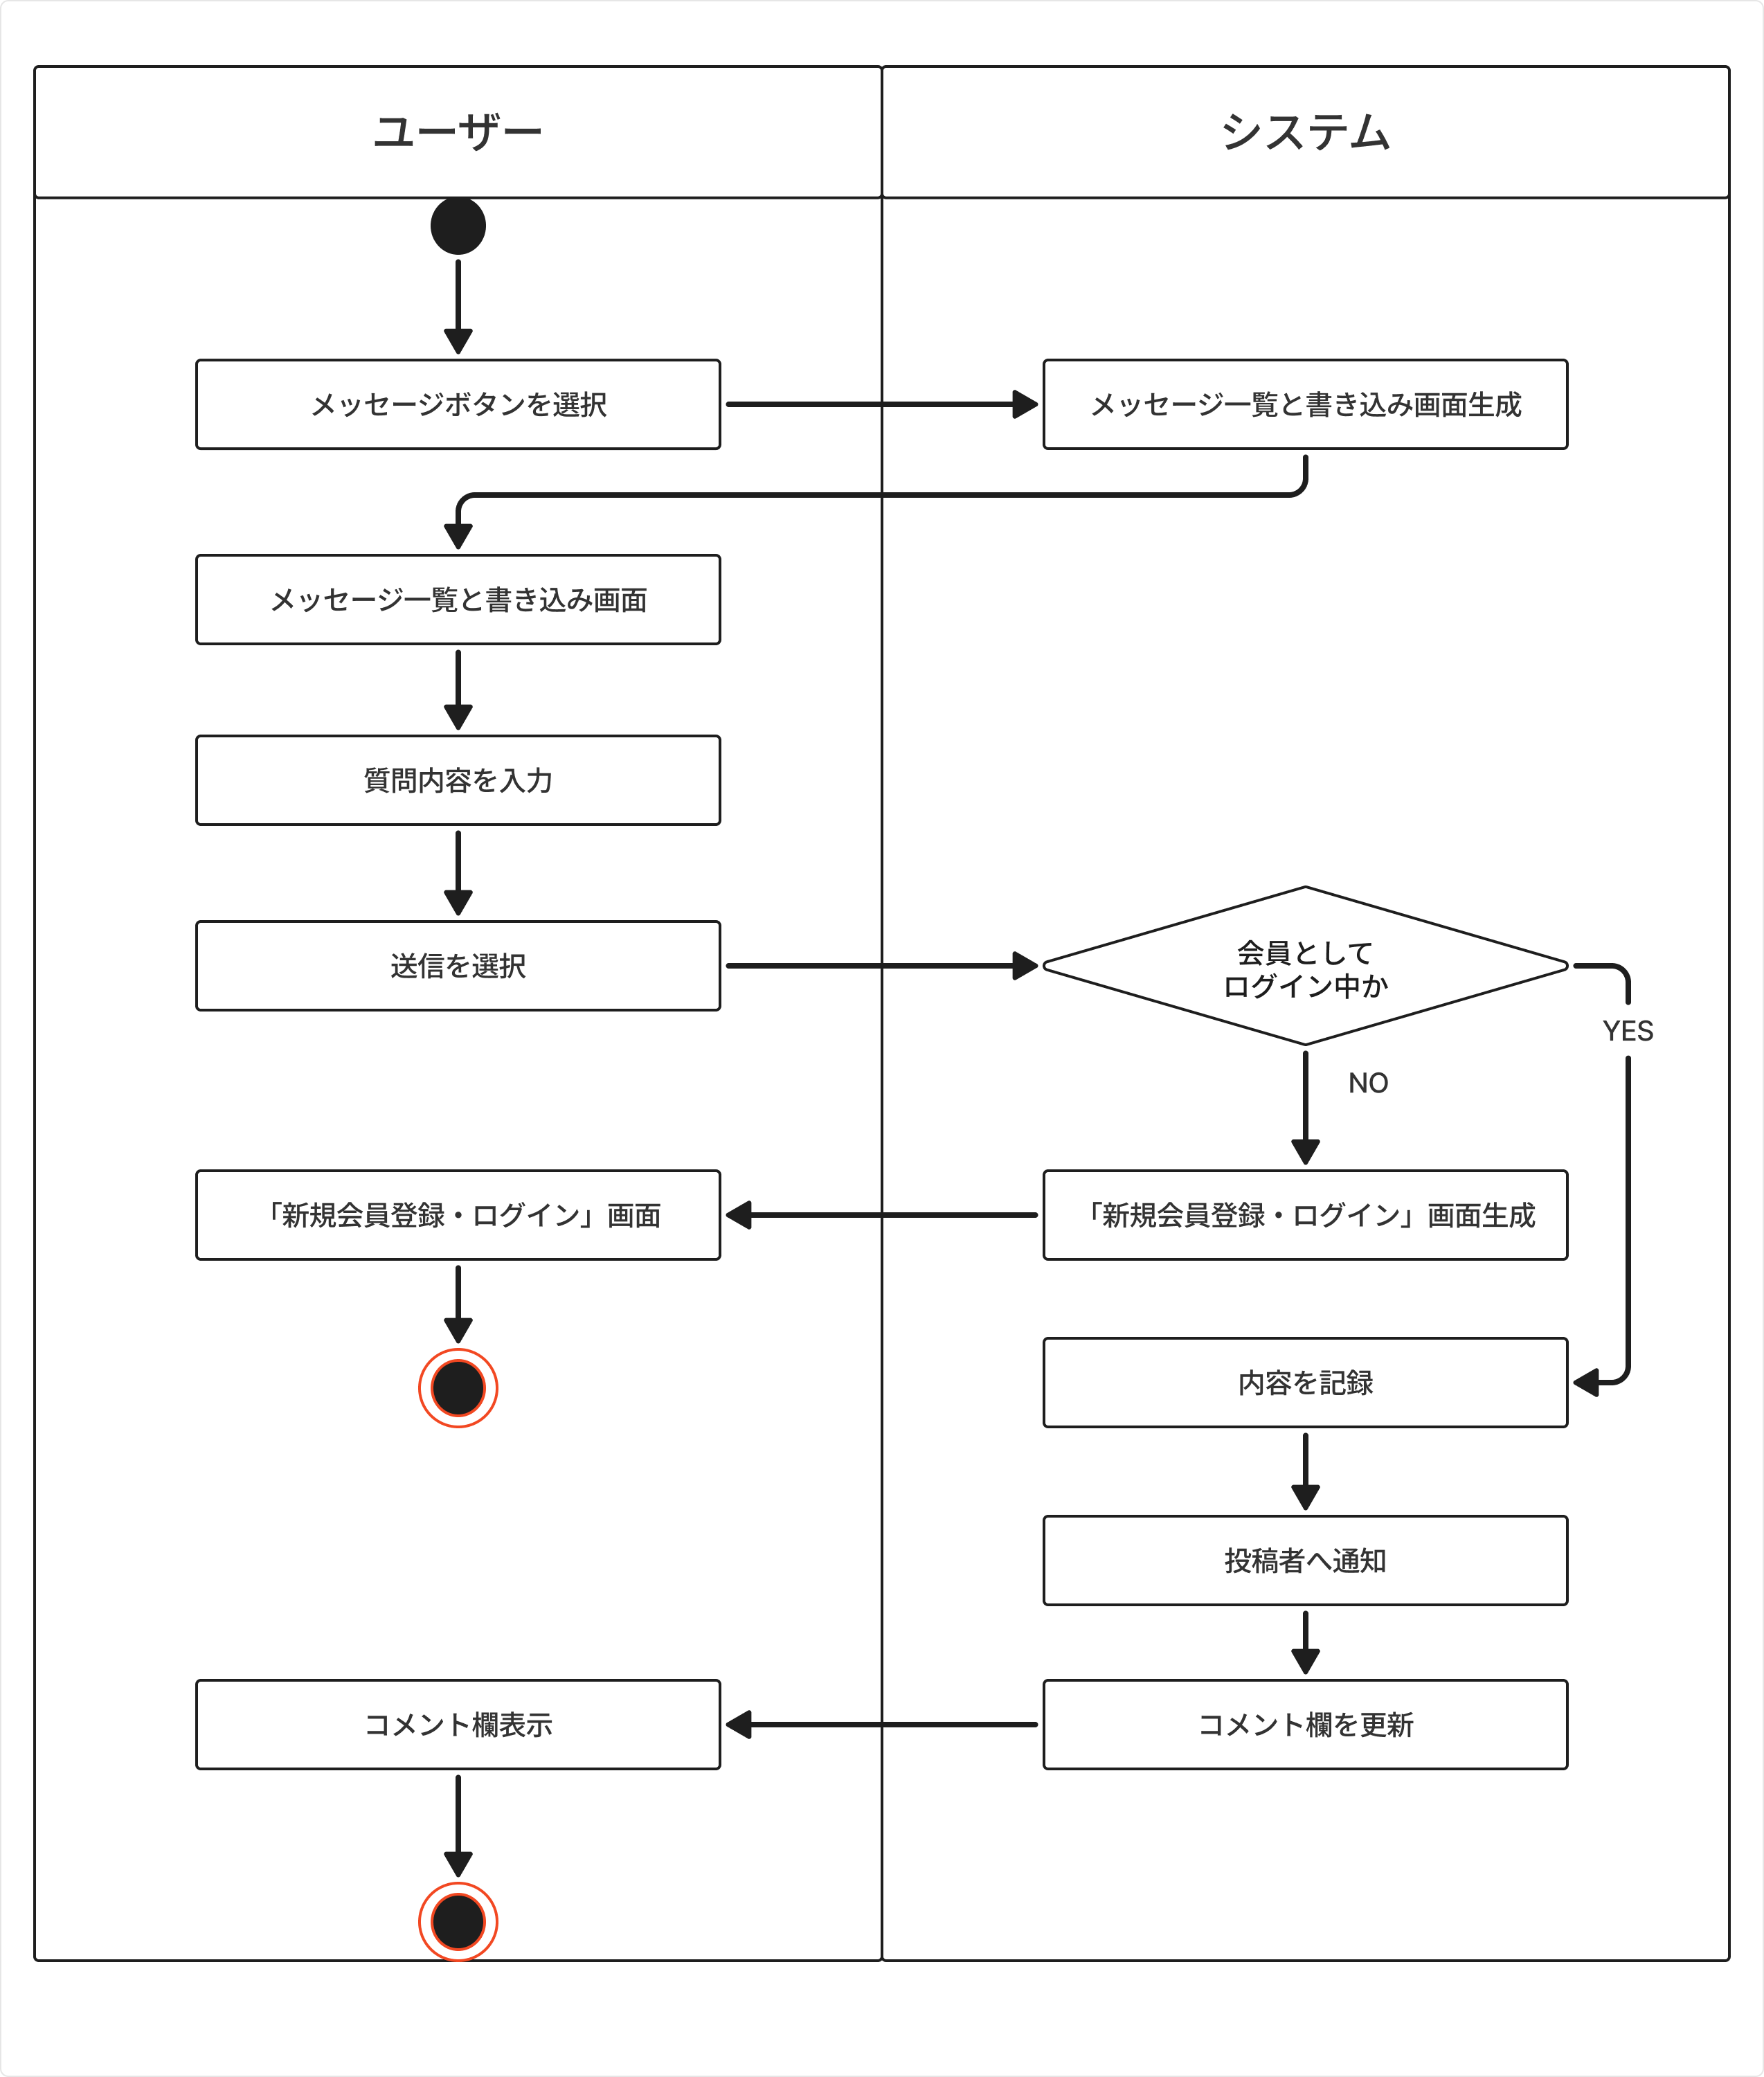
\includegraphics[width=\linewidth]{chapters/images/reply.png}
    \caption{返信機能のアクティビティ図}
    \label{fig:reply}
  \end{minipage}
  \hfill
  \begin{minipage}[t]{0.48\linewidth}
    \centering
    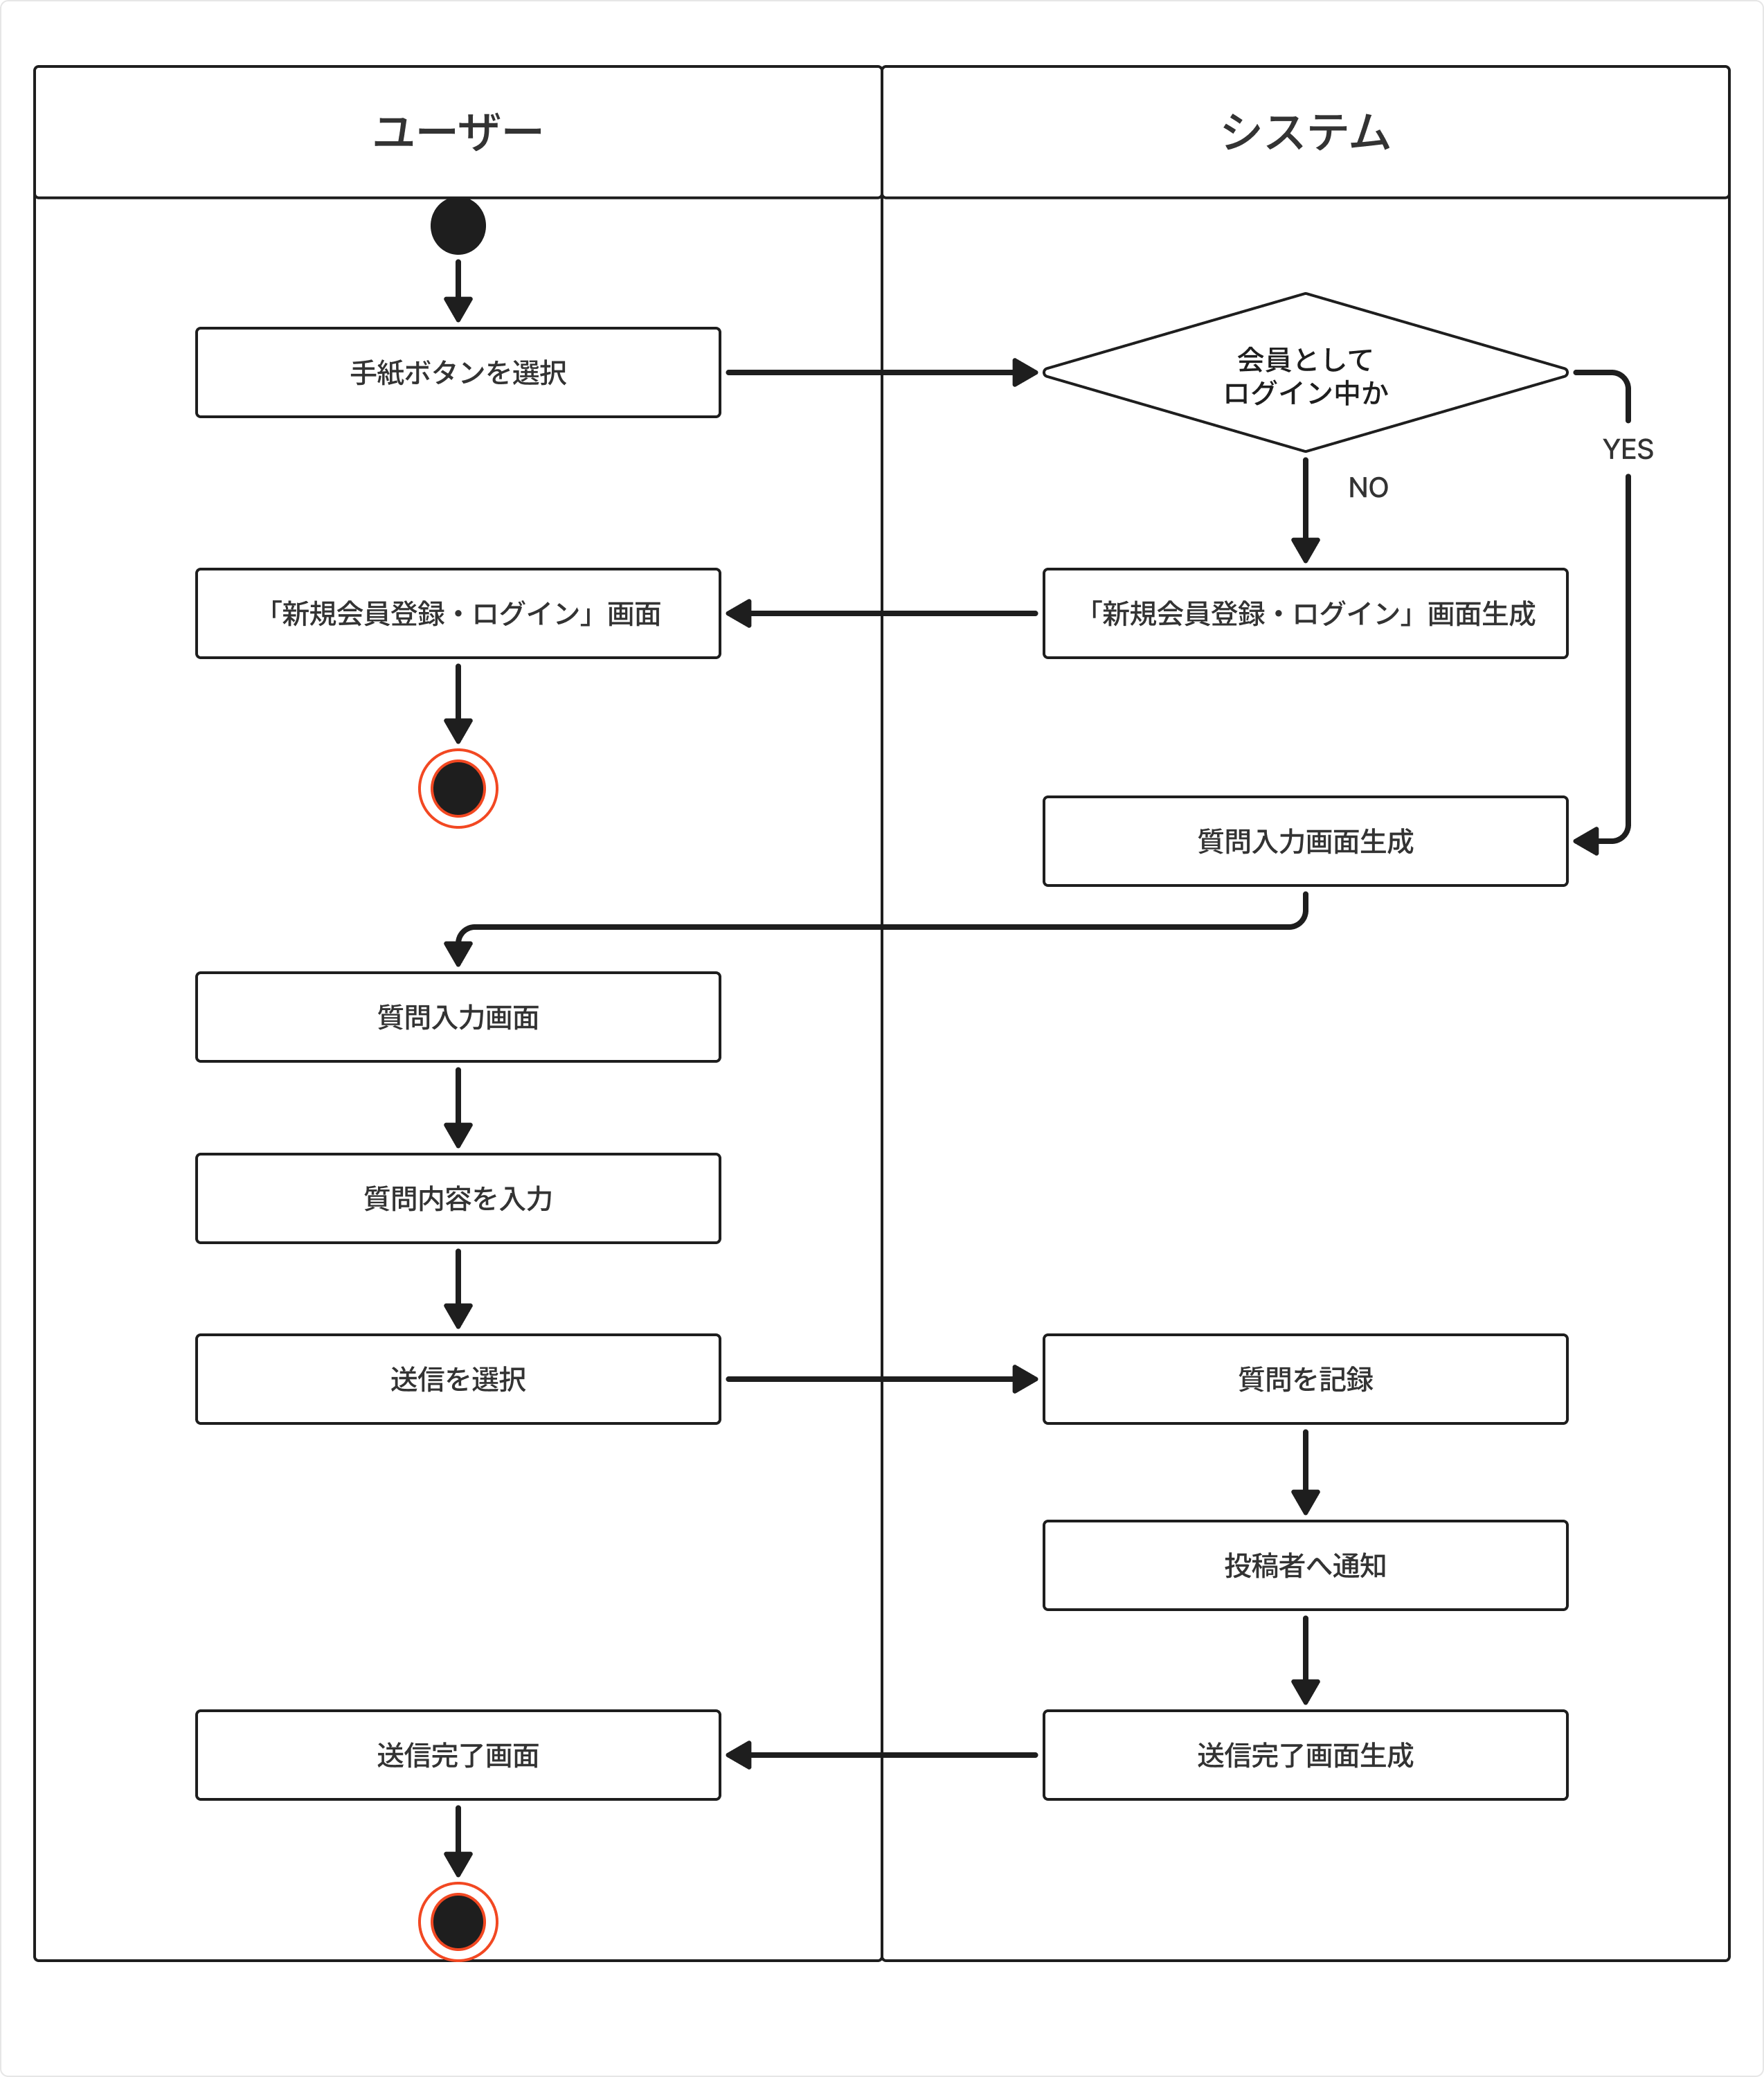
\includegraphics[width=\linewidth]{chapters/images/question.png}
    \caption{質問機能のアクティビティ図}
    \label{fig:act-question}
  \end{minipage}
\end{figure}

%......................................................................
\subsubsection{キャラクター交流・育成機能}\label{subsubsec:character}
%......................................................................
ユニコーンをモチーフにした複数のキャラクターと交流し, 育成する機能である.
利用者はユニコインを消費して, キャラクターの着せ替えアイテム, 新しいキャラクター, 背景を購入できる.
キャラクターは定型文で話しかけ, スマートフォンに関する豆知識を伝えることで, 学習意欲を高める.

図\ref{fig:character}にキャラクター交流・育成機能の流れを示す.

%......................................................................
\subsubsection{ミニゲーム機能}\label{subsubsec:minigame}
%......................................................................
フリック入力など, スマートフォンの基本操作をゲーム形式で練習する機能である.
マイページのミニゲームルームへのボタンから遷移し, ミニゲームの一覧から遊びたいゲームを選ぶ.
ゲームのスコアに応じて, ユニコインを獲得できる.

図\ref{fig:act-minigame}にミニゲーム機能の流れを示す.

\begin{figure}[H]
  \centering
  \begin{minipage}[t]{0.48\linewidth}
    \centering
    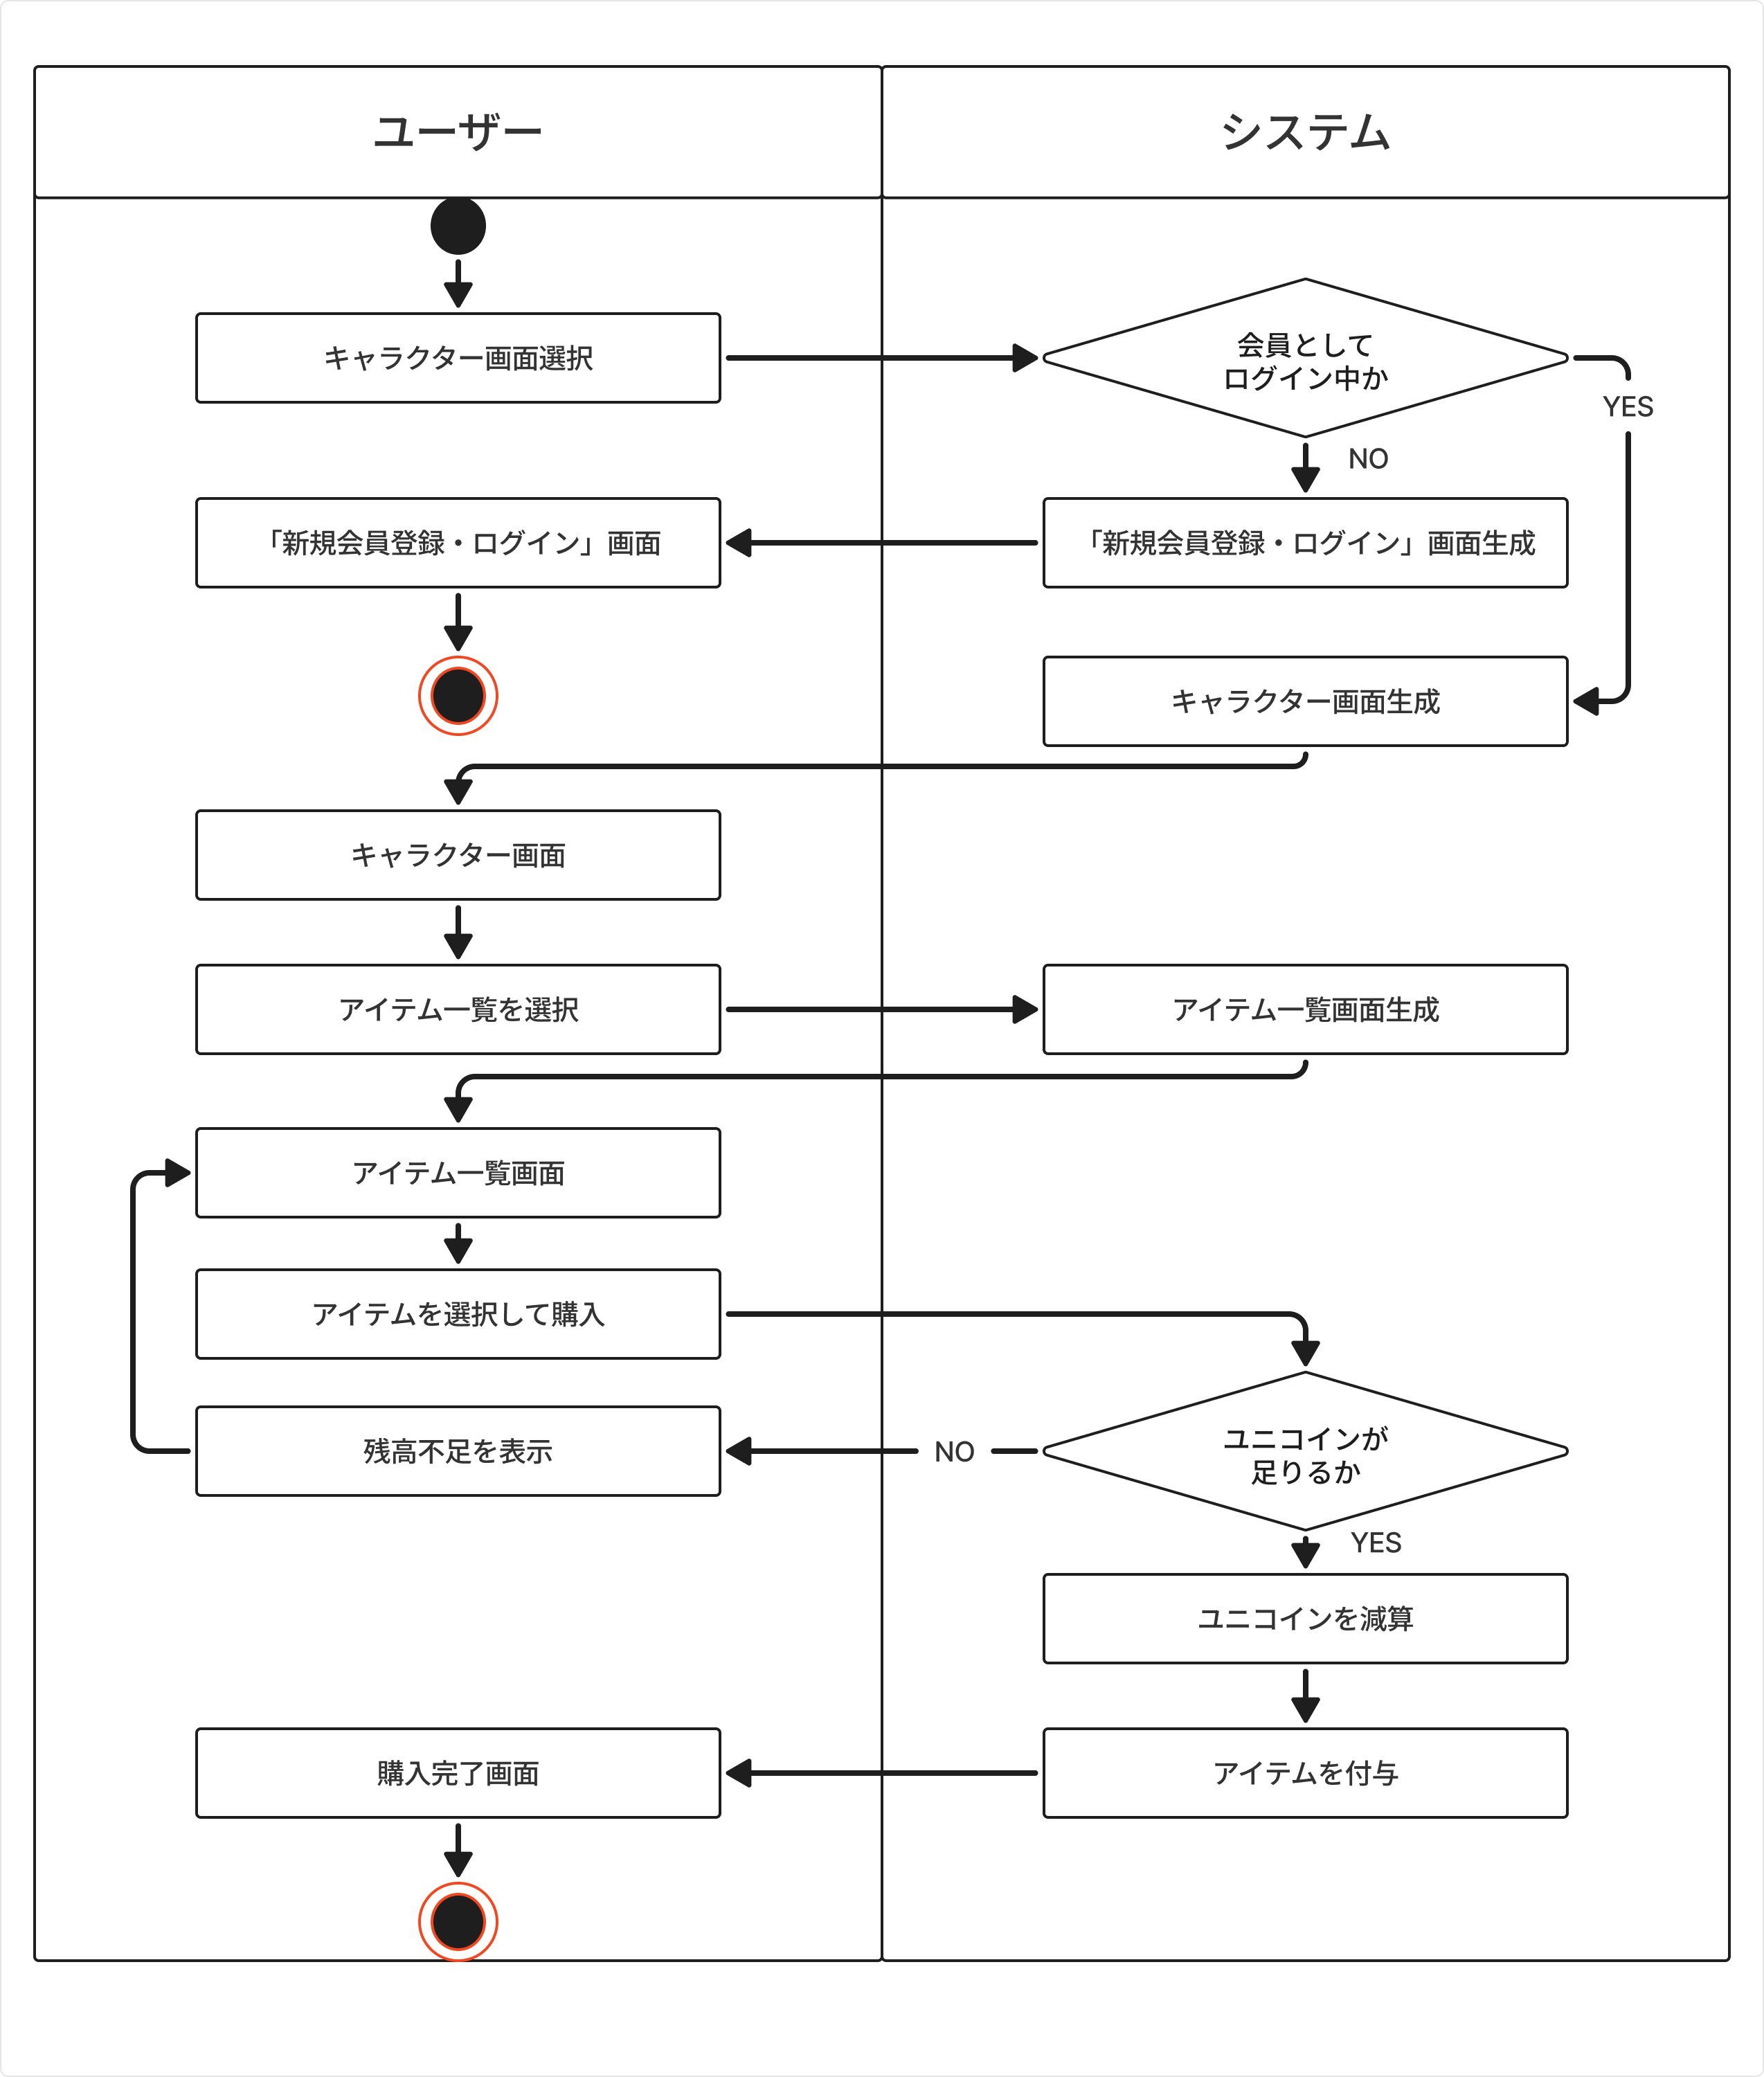
\includegraphics[width=\linewidth]{chapters/images/character.png}
    \caption{キャラクター交流・育成機能のアクティビティ図}
    \label{fig:character}
  \end{minipage}
  \hfill
  \begin{minipage}[t]{0.48\linewidth}
    \centering
    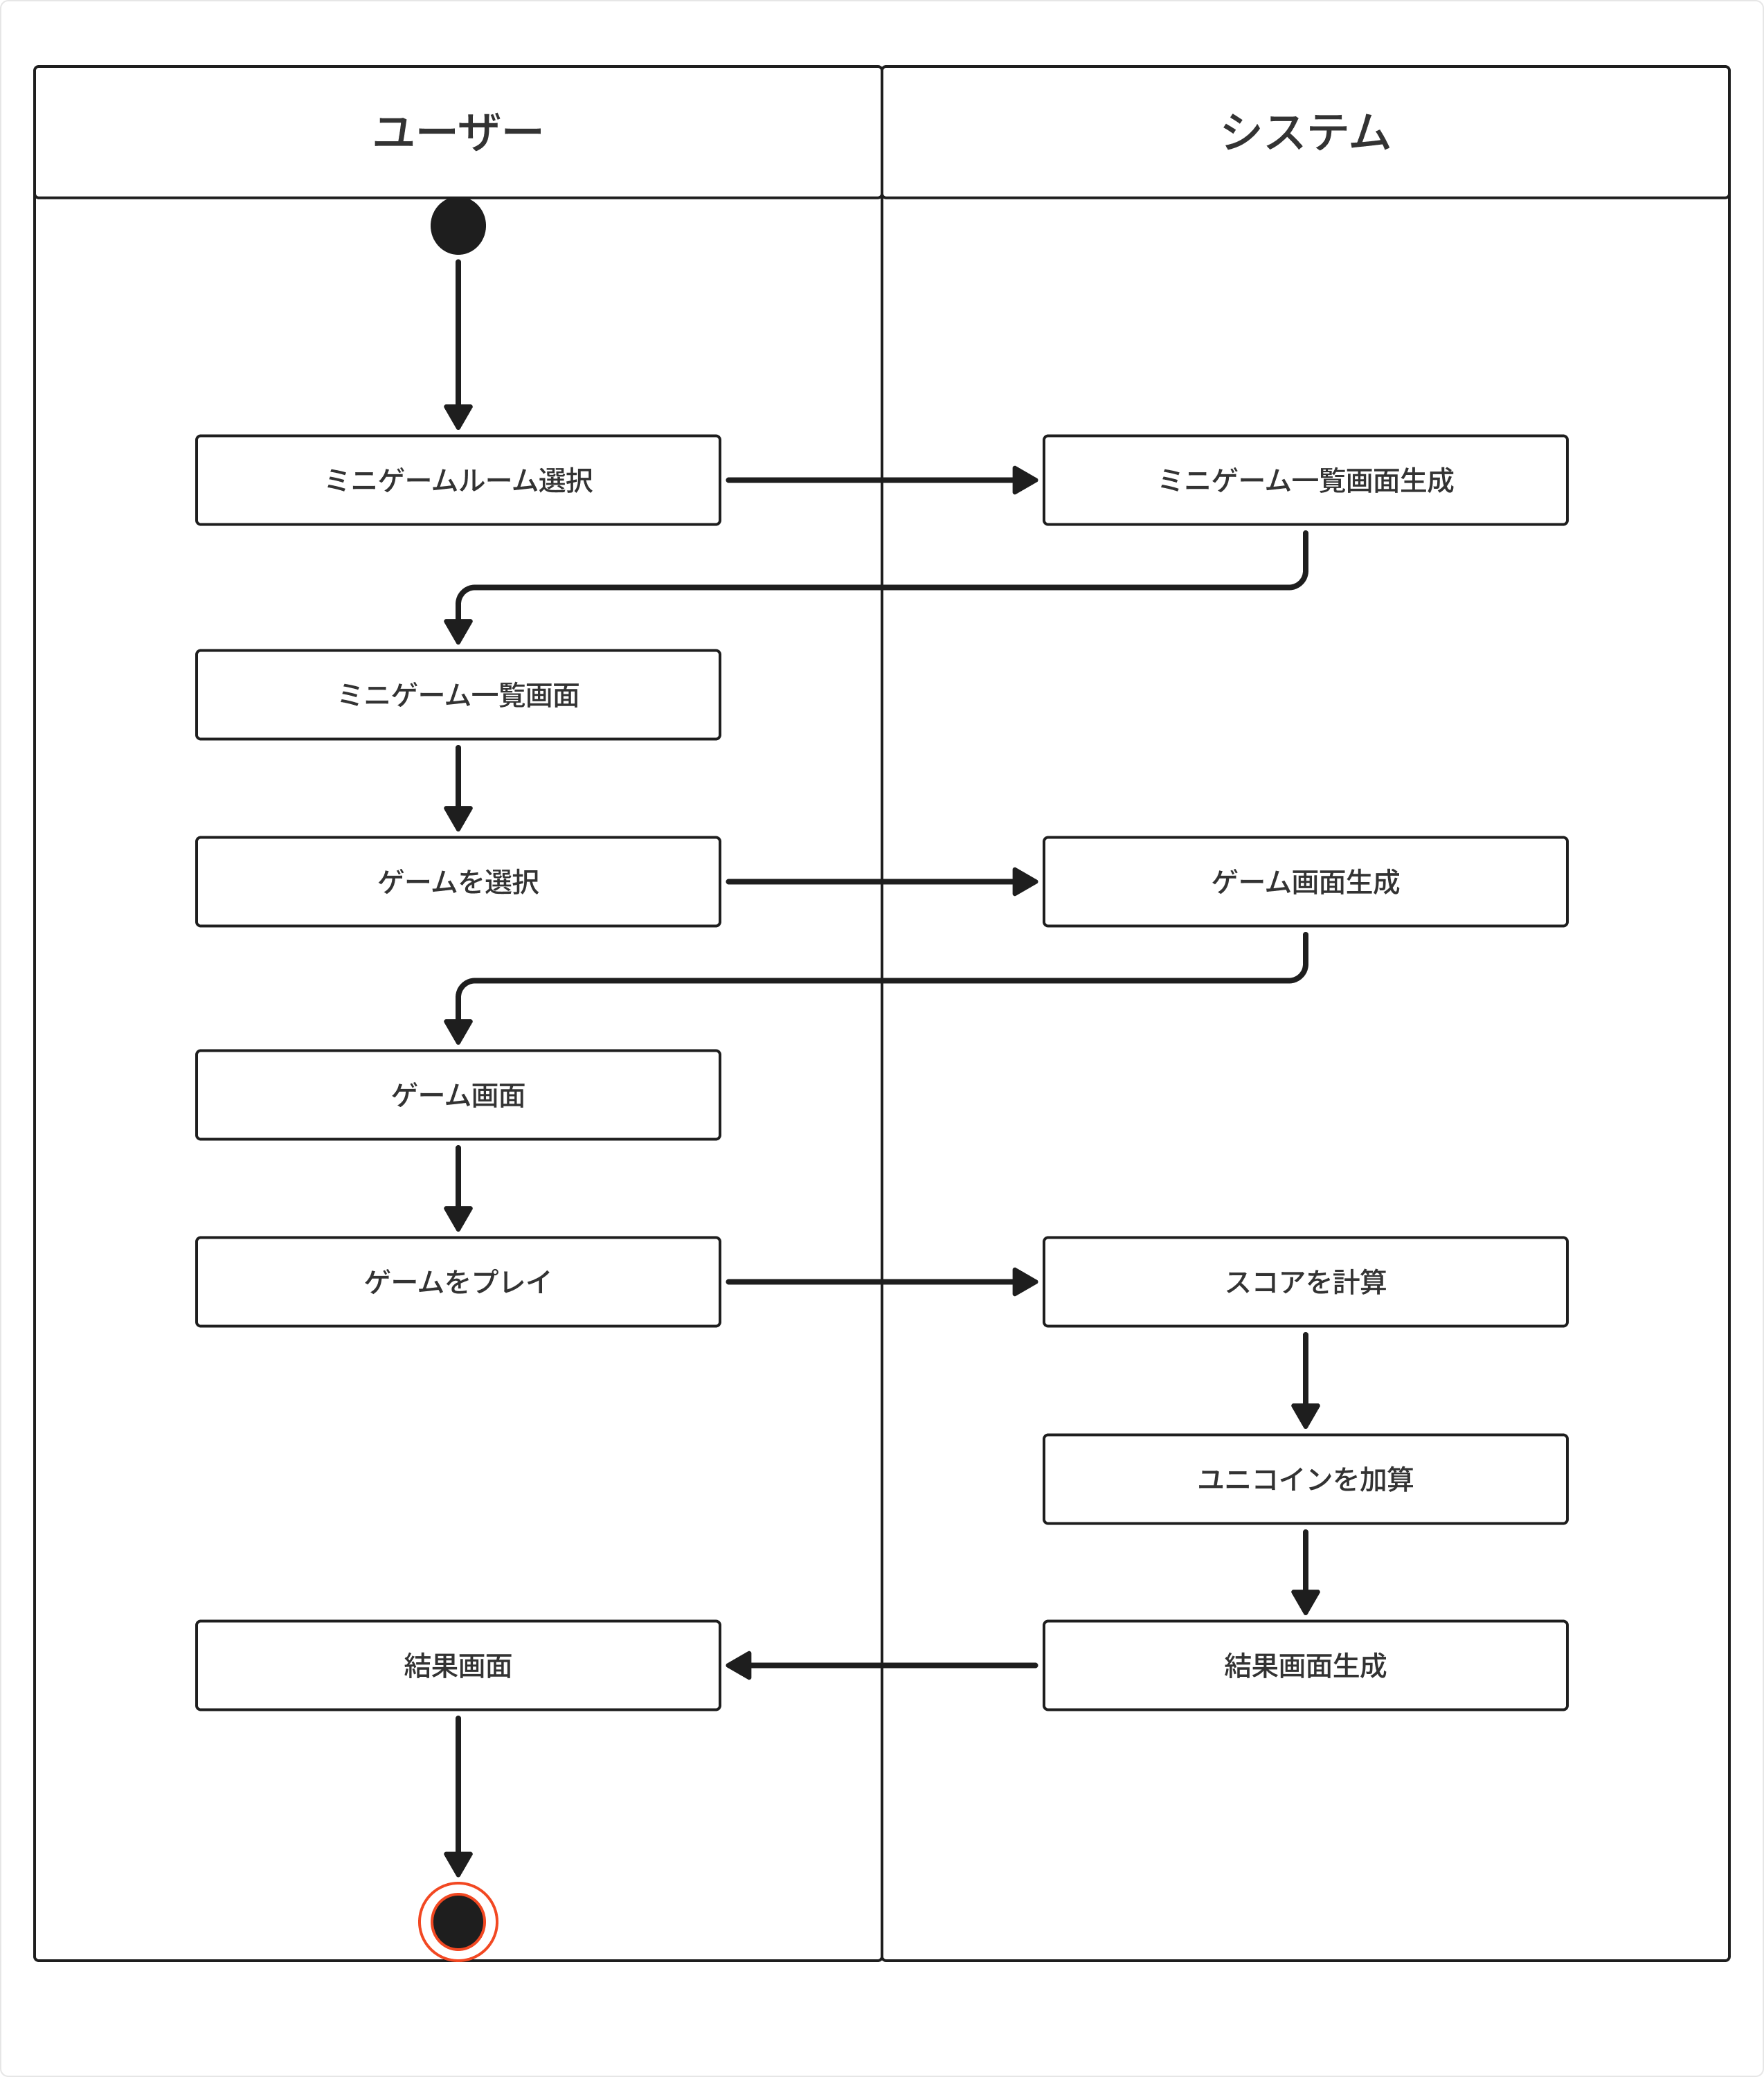
\includegraphics[width=\linewidth]{chapters/images/minigame.png}
    \caption{ミニゲーム機能のアクティビティ図}
    \label{fig:act-minigame}
  \end{minipage}
\end{figure}

%......................................................................
\subsubsection{ログインボーナス機能}\label{subsubsec:login-bonus}
%......................................................................
会員がログインしたときに, 一定数のユニコインを支給する機能である.
支給されたユニコインは, キャラクターのアイテム購入（\ref{subsubsec:character}）に利用できる.

図\ref{fig:login-bonus}にログインボーナス機能の流れを示す.


\begin{figure}[H]
  \centering
  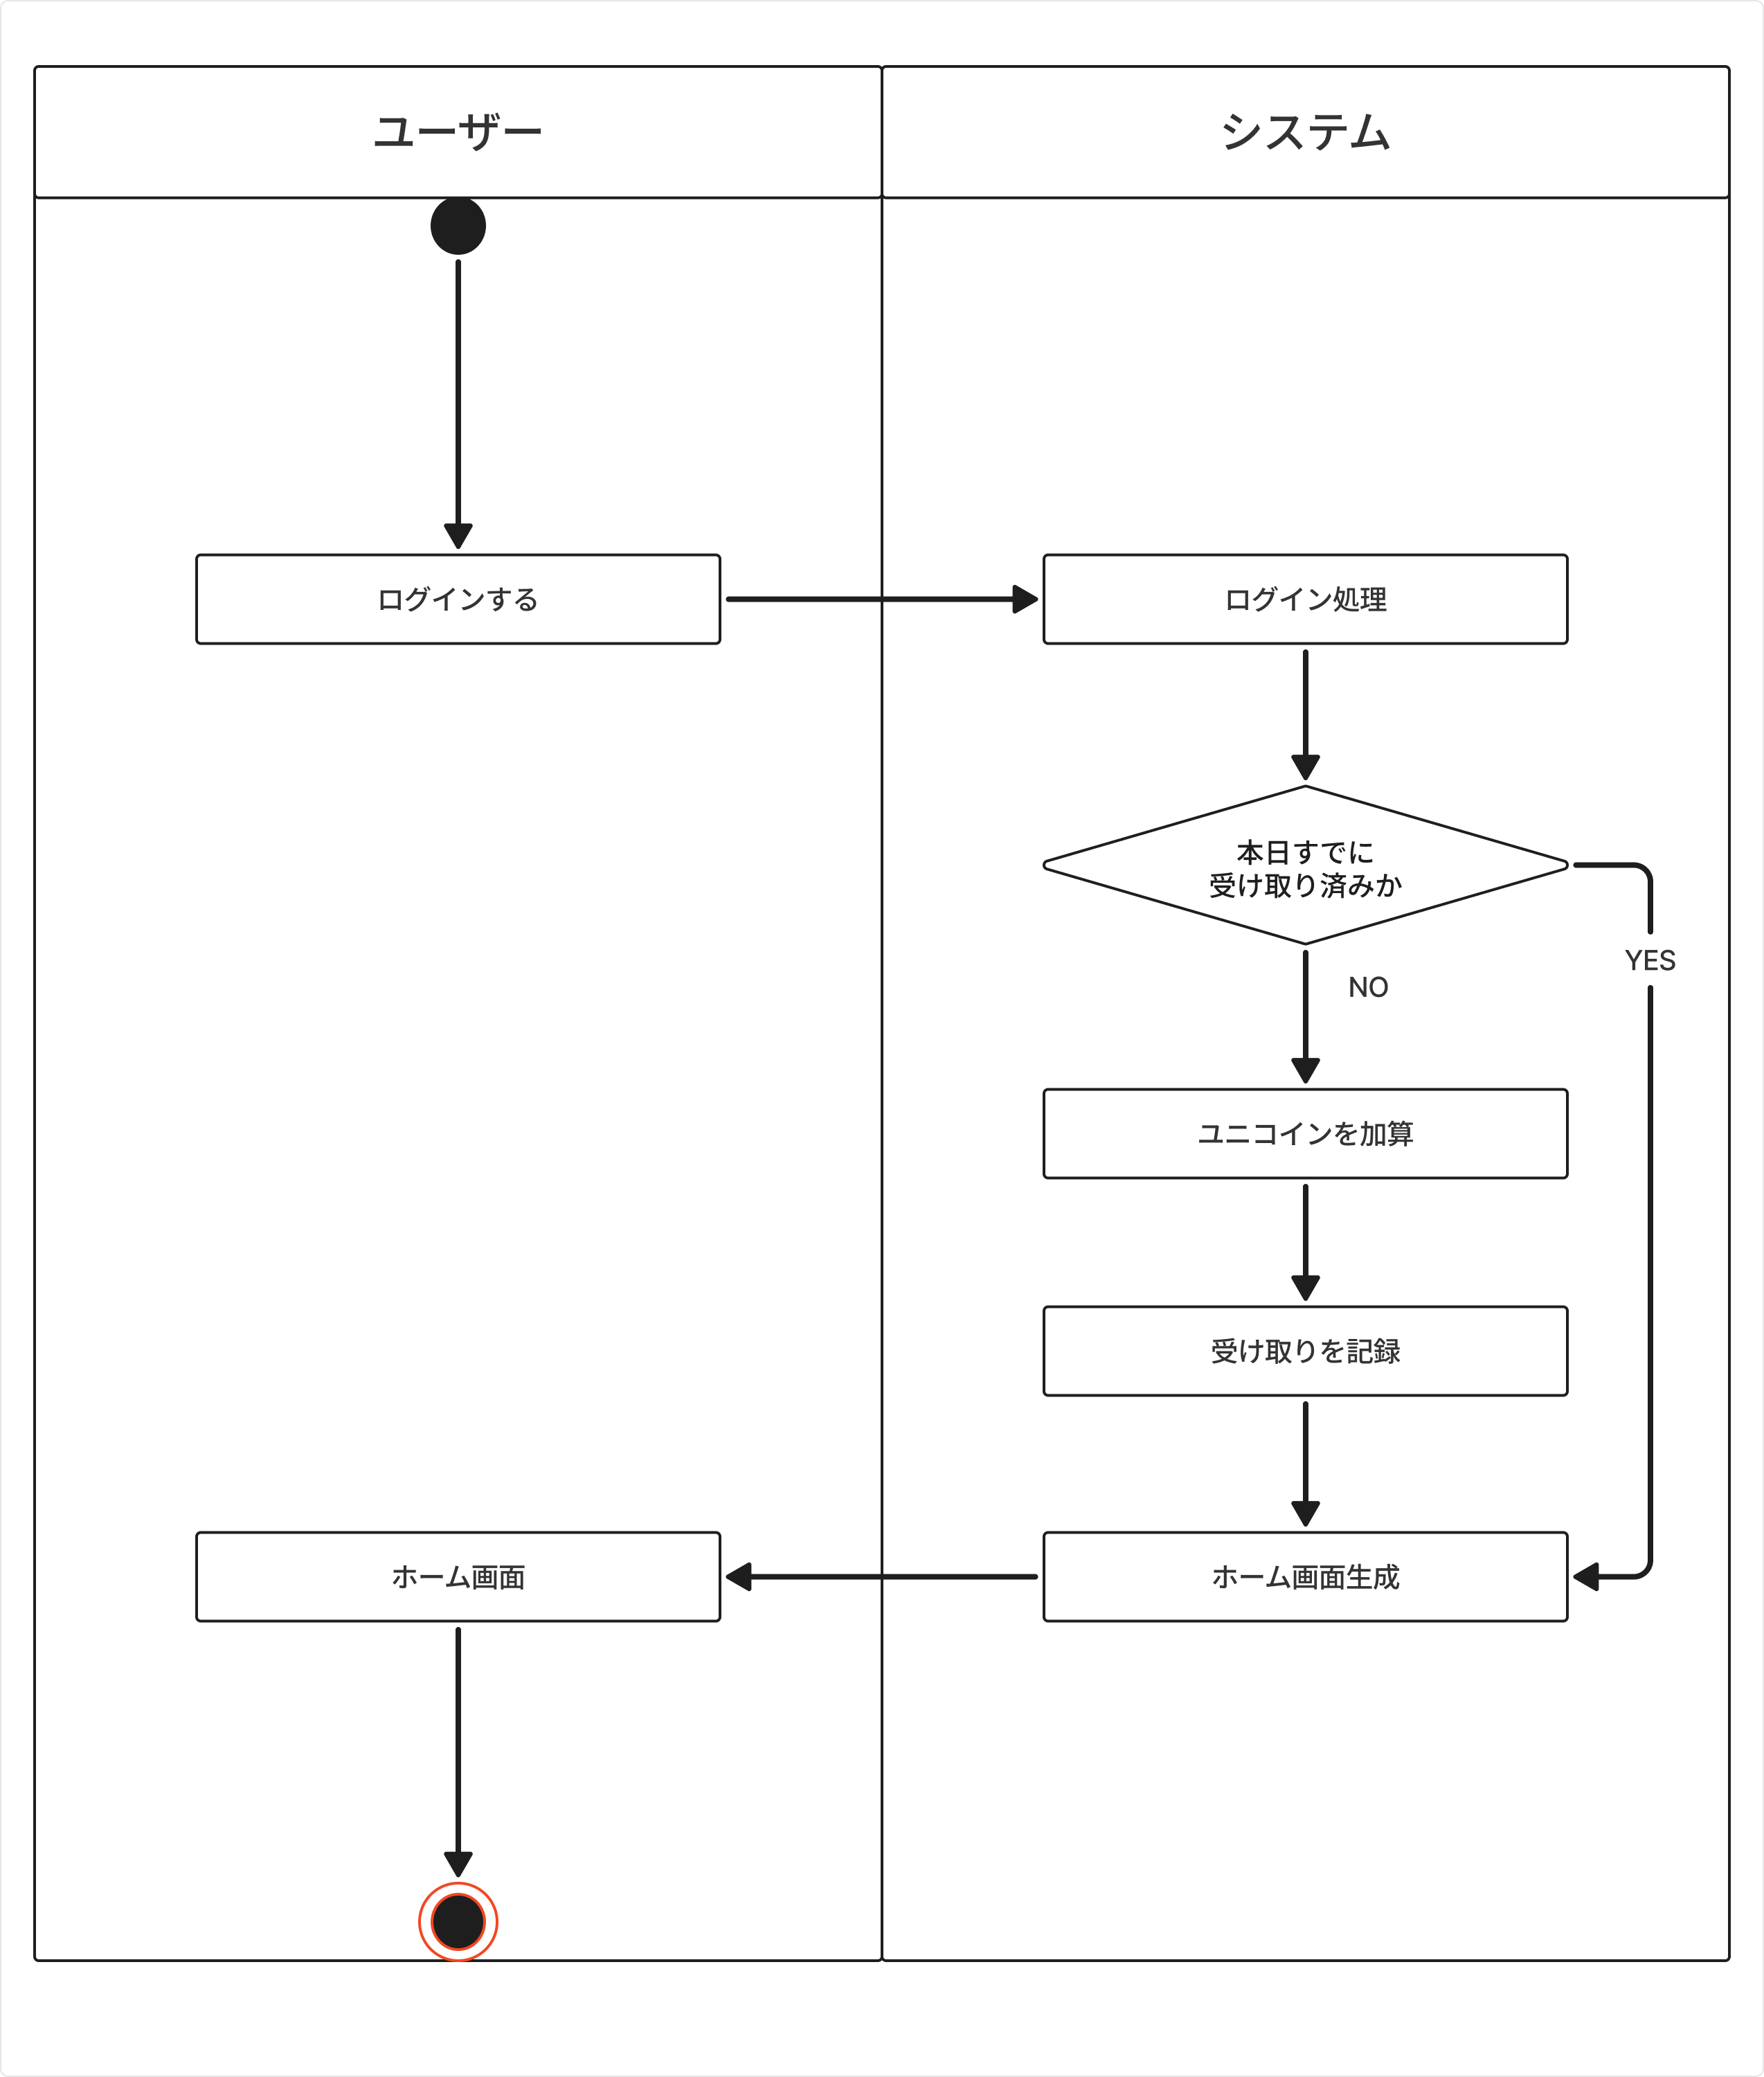
\includegraphics[width=0.48\linewidth]{chapters/images/login_bonus.png}
  \caption{ログインボーナス機能のアクティビティ図}
  \label{fig:login-bonus}
\end{figure}